%%%%%%%%%%%%%%%%%%%%%%%%%%%%%
% University of Cincinnati Thesis Template v1.1
% Author: Xiahua Liu
% Date: 10/13/2024
% License: CC0 (no copyright reserved)
%
% LaTeX is the de facto standard for the communication and publication of scientific documents and is available as free software.
% In LaTeX, you mark up the text with different tags. Opposed to "What you see is what you get" , LaTeX will arrange the text and things like links, cross references, citations for you during compilation, it makes you focus on the content itself rather than the format.
%
% This template is well scripted and is pretty straight forward in almost every thing.
% It is designed to use only necessary packages, and giving the user flexibility to add more features if needed.
%%%%%%%%%%%%%%%%%%%%%%%%%%%%%

\documentclass[11pt, twoside]{report}

%% Encoding Settings
\usepackage[T1]{fontenc}

%% Figure Settings 
\usepackage{graphicx}
\graphicspath{{images/}} % Default picture folder

%% Math packages
\usepackage{amsmath}
\usepackage{gensymb} % More symbols like \degree

%% Misc packages
\usepackage{appendix} %self explanatory
\usepackage{caption} %allows captions for graphics
\usepackage[nottoc]{tocbibind} %adds the bibliography to the table of contents
\usepackage{subcaption} %allows subcaption for multiple images in one graphic

%% Code Highlighting
\usepackage{minted}

%% Hyperlinks
\usepackage[hyphens]{url} % Break long URL in Bib by hyphens
\usepackage{hyperref}
\hypersetup{colorlinks=false} % No blue link texts!

%% Page Margin Settings
\usepackage[letterpaper, top=1in, bottom = 1in, right = 1in]{geometry}

\begin{document}

%%%%%%%%%%%%%%%%%%%%%%%%%%%%%%%%%%%%%%%%%%%
% Preamble
%%%%%%%%%%%%%%%%%%%%%%%%%%%%%%%%%%%%%%%%%%%

\begin{titlepage}
    \begin{center}
        \vspace*{0.8cm}
        % Title Name Here. DO NOT use all capital letters for your title. 
        % Portions of all CAPS in the title are still appropriate for acronyms, proper nouns, first letter, etc.
        % If the title takes multiple lines, you should manually break the title with "\\" 
        % and control the text on each line. Be sure to add an extra return "\\" before "}" 
        
        {\LARGE \selectfont \bfseries
            Piranha: An Autonomous Water Surface Robot \\
            %I am the second line in case you need \\
            %I am the third line in case you need \\
            %You probably do not want a forth line \\
        }

        % Vertical fill here, you can think this as a spring spacer between the upper and lower parts,
        % it pushes the rest of page to align with the bottom. 
        \vfill
        
        % This should be the same for all programs
        % Font size is 12pt, baseline skip is 24pt (double spacing)
        {\fontsize{12pt}{24pt}\selectfont
        A thesis submitted to the \\
        Graduate School \\
        of the University of Cincinnati \\
        in partial fulfillment of the \\
        requirements for the degree of \\
        
        % Vertical space
        \vspace{1cm}
        
        % Your degree
        Master of Science
        
        % Vertical space
        \vspace{1cm}
        
        % Your department
        in the Department of Aerospace \\ 
        Engineering \& Engineering Mechanics \\
        by \\
        
        % Vertical space
        \vspace{1cm}
        
        % Your name
        Xiahua Liu \\
        
        \vspace{2cm}
        }
        
        % Your previous degree and school.
        % Font size is 12pt, baseline skip is 24pt (double spacing)
        {\fontsize{12pt}{24pt}\selectfont
        
        B.S. Beijing Institute of Technology \\
        
        % Date
        June, 2018 \\
        
        % Vertical space
        \vspace{1cm}
        
        % Committee Chair name
        Committee Chair: Ou Ma, Ph.D. \\
        }
        
        % Vertical space
        \vspace{0.8cm}
 
    \end{center}
\end{titlepage}

\pagenumbering{roman}
%Roman numbering is recommended until the body

% The preamble section is double spacing.
\renewcommand{\baselinestretch}{2}\selectfont

% Abstract page
\chapter*{Abstract}

This thesis describes the design and development work of a marine debris cleanup system - Piranha. It is an autonomous water surface vehicle that can collect different types of garbage such as plastic bottles and bags. To begin with, Piranha is simple, with minimum moving parts including only two thrusters and a lever system. Necessary sensors like IMUs and GPS on Piranha enable positioning and navigation functions. Besides sensors, a LoRa wireless module allows the human worker to control Piranha from a distance. The simulation software for Piranha is discussed in chapter four with the theoretical equations and numerical methods. In the end, some control algorithms, including a 13 state EKF, a heading controller, and a trajectory tracking controller, are brought up to achieve autonomy at a certain level. This report reveals the development cycle of Piranha, from the very simple low-level mechanical parts to the high-level robotics system design.

% Blank page
\clearpage

% Acknowledge page
\chapter*{Acknowledgements} %the star makes the chapter unnumbered

First of all, I want to thank the project founder, Michael Arens. He provided the idea and named this project. Without him, the project would not exist. 

During the control system design, Jonathan and Krishna provided their opinions and suggestions to me. However, it almost ended up in a fight because we could not agree with each other. As a result, I combined their ideas, meanwhile absorbed the advantages of different existing techniques into the final control system design.

Byron Castillo, currently a Mechanical Engineering student at the University of Cincinnati, finishes the mechanical design part. Benjamin Russ is the industrial designer for the product, and he also took part in the mechanical design of Piranha.

In the end, I also want to thank the University of Cincinnati 1819 Innovation Hub and Ben Jones, the Makerspace Manager. They provided the workspace for us and also funded this project.

During my two years of study at the University of Cincinnati, Prof. Ou Ma, Prof. Donghoon Kim, Prof. Janet Dong, and Prof. Shaaban Abdallah in the College of Applied Engineering and Science had generously shared the professional knowledge with me. This invaluable knowledge and experience helped all the work done in this project.

% The Table of Content is single spacing.
\renewcommand{\baselinestretch}{1}\selectfont

% Set table of content depth to 4 to ensure all subsubsections and paragraphs are collected
\setcounter{tocdepth}{4}

\tableofcontents

\listoffigures

\listoftables

\newpage

\pagenumbering{arabic}
%back to Arabic numbering for the rest

%%%%%%%%%%%%%%%%%%%%%%%%%%%%%%%%%%%%%%%%%%%
% Chapters
%%%%%%%%%%%%%%%%%%%%%%%%%%%%%%%%%%%%%%%%%%%

% The main text is double line spacing.
\renewcommand{\baselinestretch}{2}\selectfont

\chapter{Introduction}

The aggressive development in the industry in the past few centuries brought humankind to an unprecedented advanced stage. We make gas-powered cars allowing us to run faster than any animals on the earth; ships carrying people cruise across the oceans every day, and even spacecraft to escape from Earth and Sun to deep space. But those brilliant achievements came with prices. One of them is the increasing number of wastes in the marine area.

\section{Background} \label{sec:background}

There is a giant plastic waste island called the Great Pacific Garbage Patch on the earth. Its size is 1.6 million $km^2$, more than twice the size of Texas (approximate 0.7 million $km^2$) \cite{Lebreton2018}. This floating waste "continent" is the outcome of the increasing amount of trash produced by industries and individuals in the past centuries and the weak effort of collecting trash in the water.

Compared with the ocean trash problem, coastal pollution is never more severe in history. According to a 2014 research, even in the most remote area on the earth, traces of plastic wastes were found \cite{Cozar10239}. It means while we enjoy using plastic forks and bottles, they have surrounded our planet silently. As factories and manufacturers increase their production, more and more plastic wastes will enter the water in the next few decades. Research shows there will be more plastic than fish in 2050 \cite{agenda2016new}. Figure \ref{fig:01plastic} shows the exact situation that plastic wastes are changing the living environment of sea creatures.

Compared with metal materials, plastic materials are superior in weight and durability and are pretty easy to form in any shape. However, this also makes plastic the most stubborn trash on the earth. Some of them cannot be decomposed in hundreds of years \cite{acssuschemeng.9b06635}. So we must take action on the marine trash collection instead of hoping them go away one day.

\begin{figure}[ht]
    \centering
    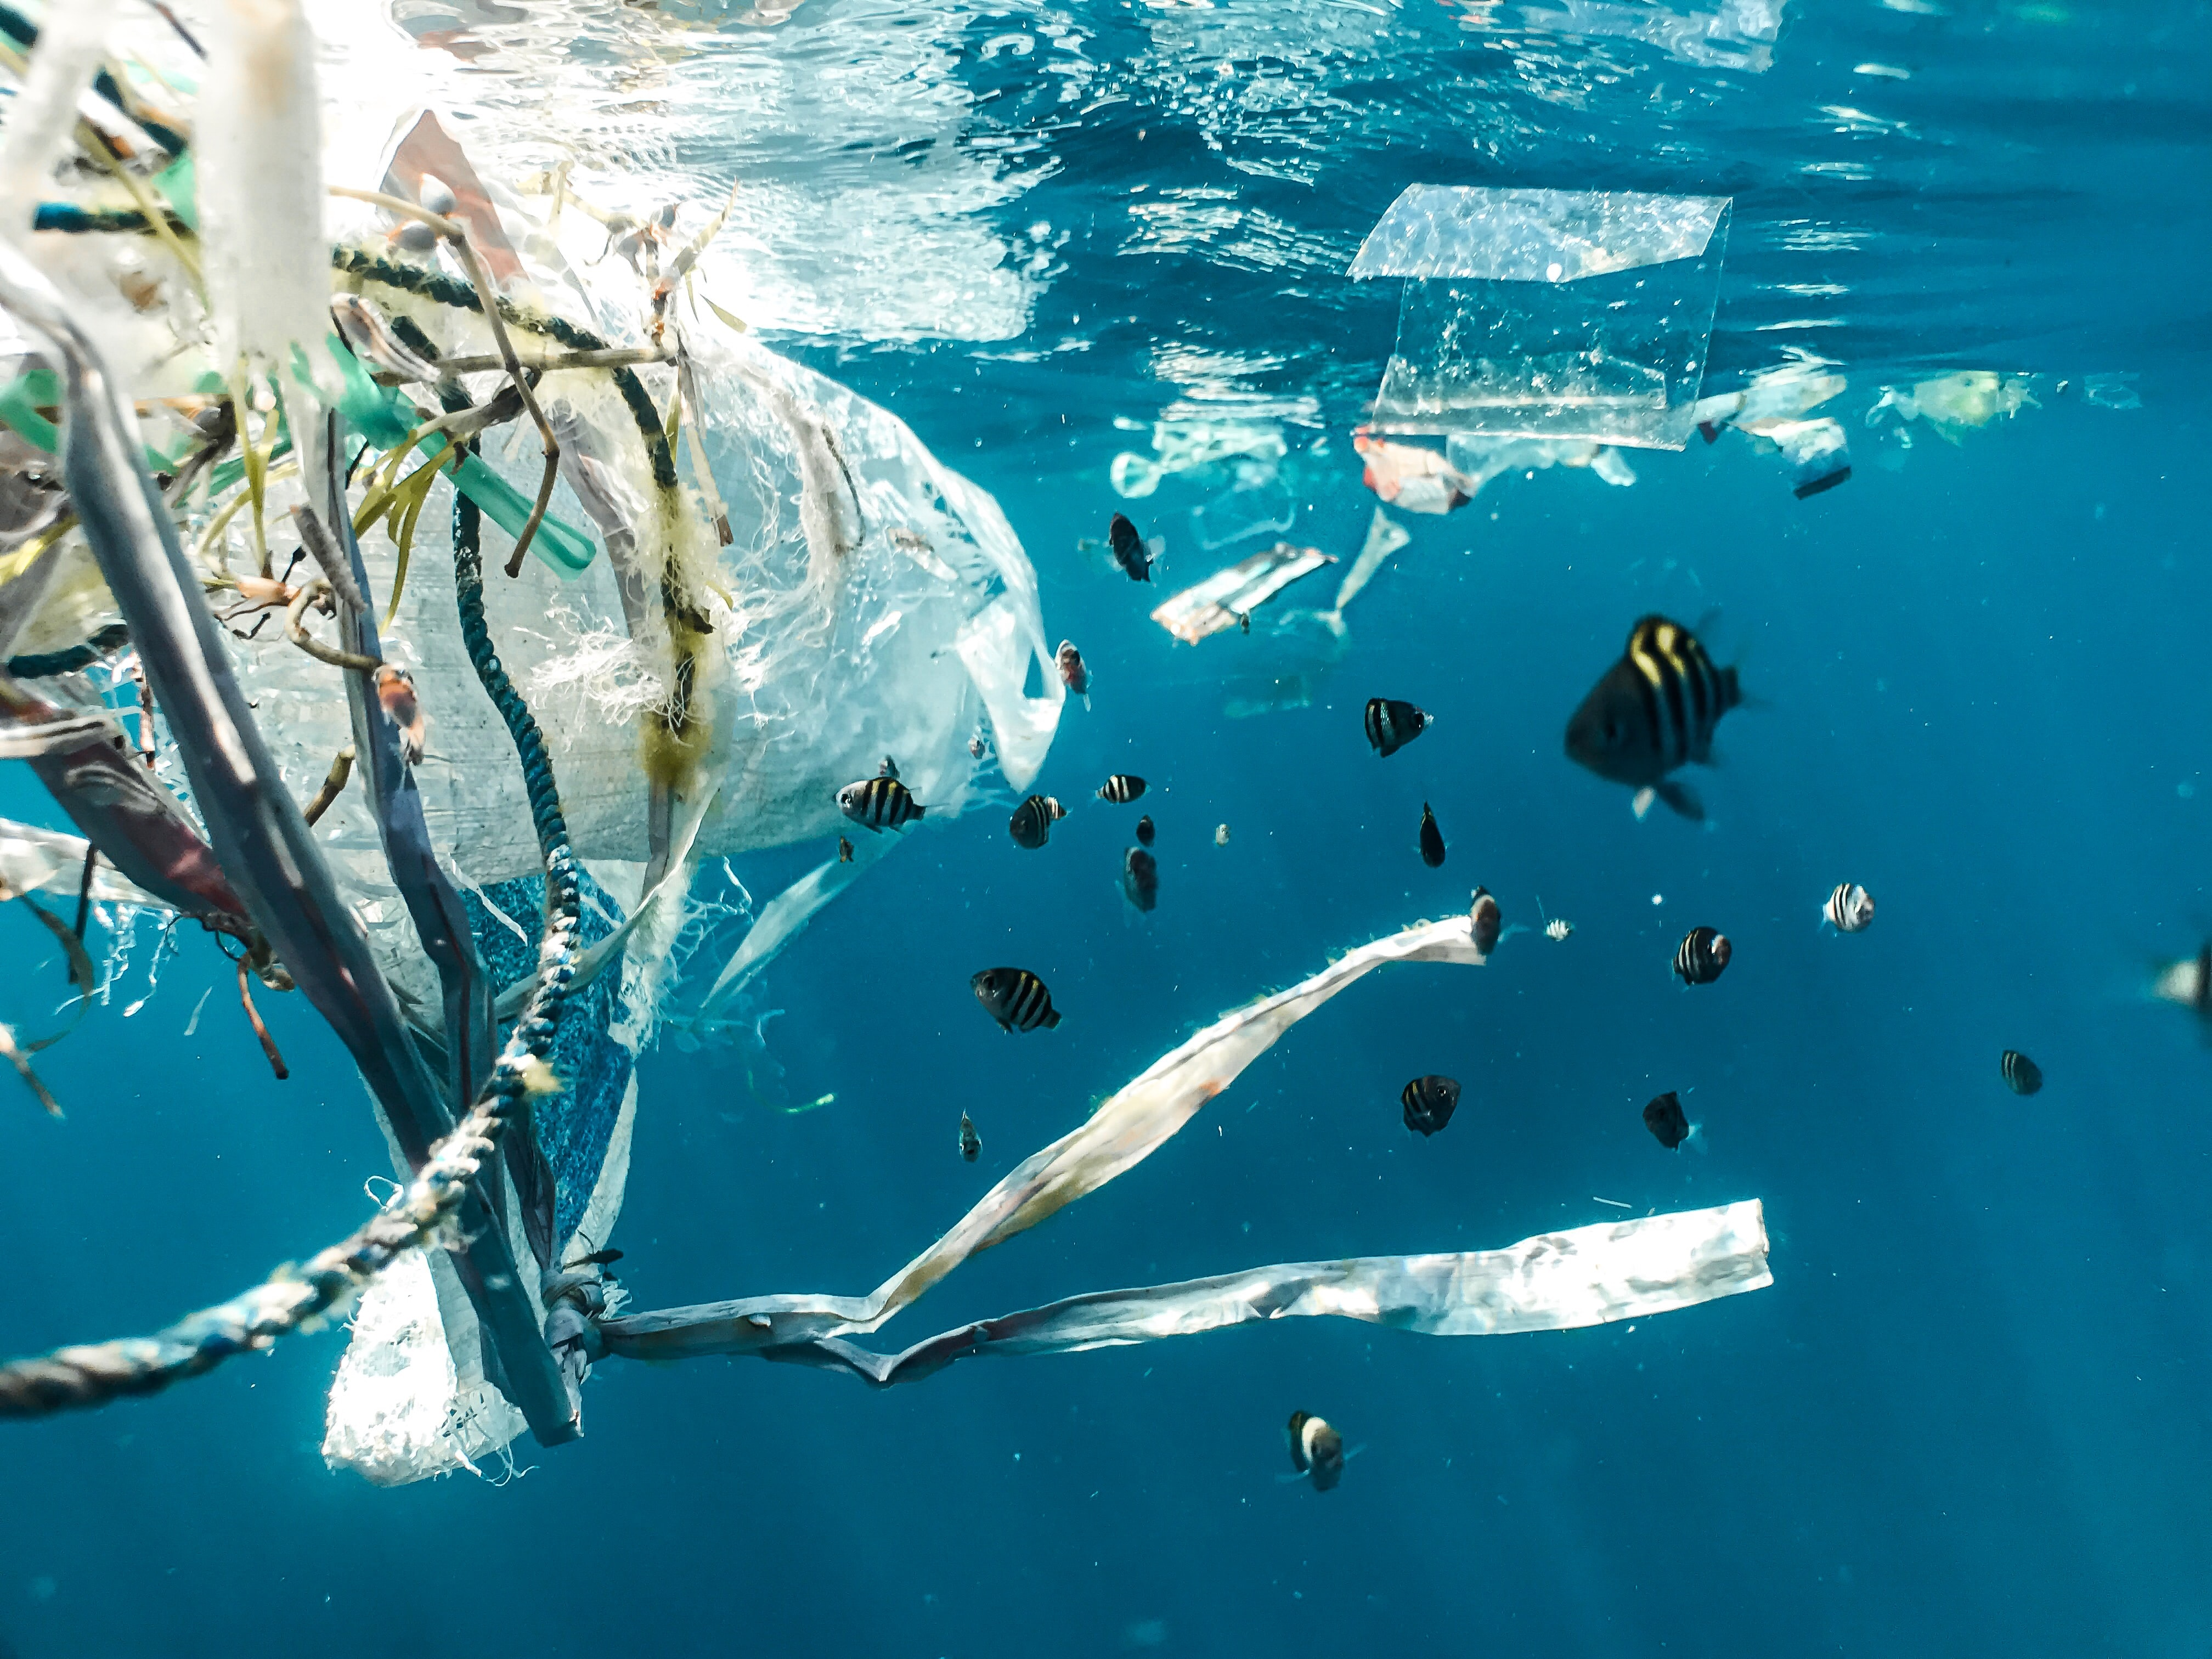
\includegraphics[width=.8\textwidth]{01plastic.jpg}
    \caption{Some fishes lives with plastic wastes in water.}
    \label{fig:01plastic}
\end{figure}

\section{Plastic harms}

Most of the marine wastes are made of plastics \cite{Lebreton2018}, as they are resistant to corrosion, oxidation, and corruption. Plastic wastes can kill sea creatures in three main ways:

\begin{itemize}
    \item \textbf{Plastic ingestion}. According to the research, fishes in the North Atlantic area ingest thousands of tons of plastic wastes every year, most of which are microplastics. These plastic grains cause intestine bleeding, which can lead sea animals to death. \cite{Davisonmeps09142}
    \item \textbf{Physical harm}.  Some sea creatures like turtles and birds do not own the ability to remove the plastic bags wrapped around their heads, and they may die of suffocation. Another example of the physical damage of plastics is the derelict nylon fishnet lines. It can entangle even giant animals like seals, whales and leave them stranded.
    \item \textbf{Block the sun light}. Tiny algae in the shallow water layer rely on the sunlight to grow and reproduce. Floating wastes block the sunlight, in turn reducing the number of algae. As a result, there is not enough food for small sea animals, the bottom residents of the food chain. The reduction in food limits the overall animal population. On the other hand, fewer plants mean less oxygen. The dissolved oxygen in water also drops, making fishes harder to breathe.
\end{itemize}

\section{Plastics on the shorelines}

There is research pointing out the vast majority of the plastics in the ocean end up washed, or buried under the shorelines, whether dry shorelines, coastal areas, or offshore areas \cite{owidplasticpollution}. However, because shorelines are long and most parts are far from human habitats, the trash collection force on shorelines is significantly less than the land. The main reason is the lack of hands and the high price of human labor.

That is why we designed Piranha. Piranha is a water surface robot that can be operated remotely by a human worker or cruise on its own to collect floating trash near the coast. It has a highly advanced control system built similarly to modern drone controllers, and we equipped it with customized control algorithms. On the mechanical side, it has a straightforward design to achieve lower building costs and higher reliability. 

Figure \ref{fig:01rendered} shows a rendered model of Piranha made in SOLIDWORKS 2017. Figure \ref{fig:01piranha} shows the overall structure of Piranha during the fourth field test. In that test, we tried using a pulley system to lift the collection bin so that human workers could easily dump the trash when the trash bin was full.

\begin{figure}[H]
    \centering
    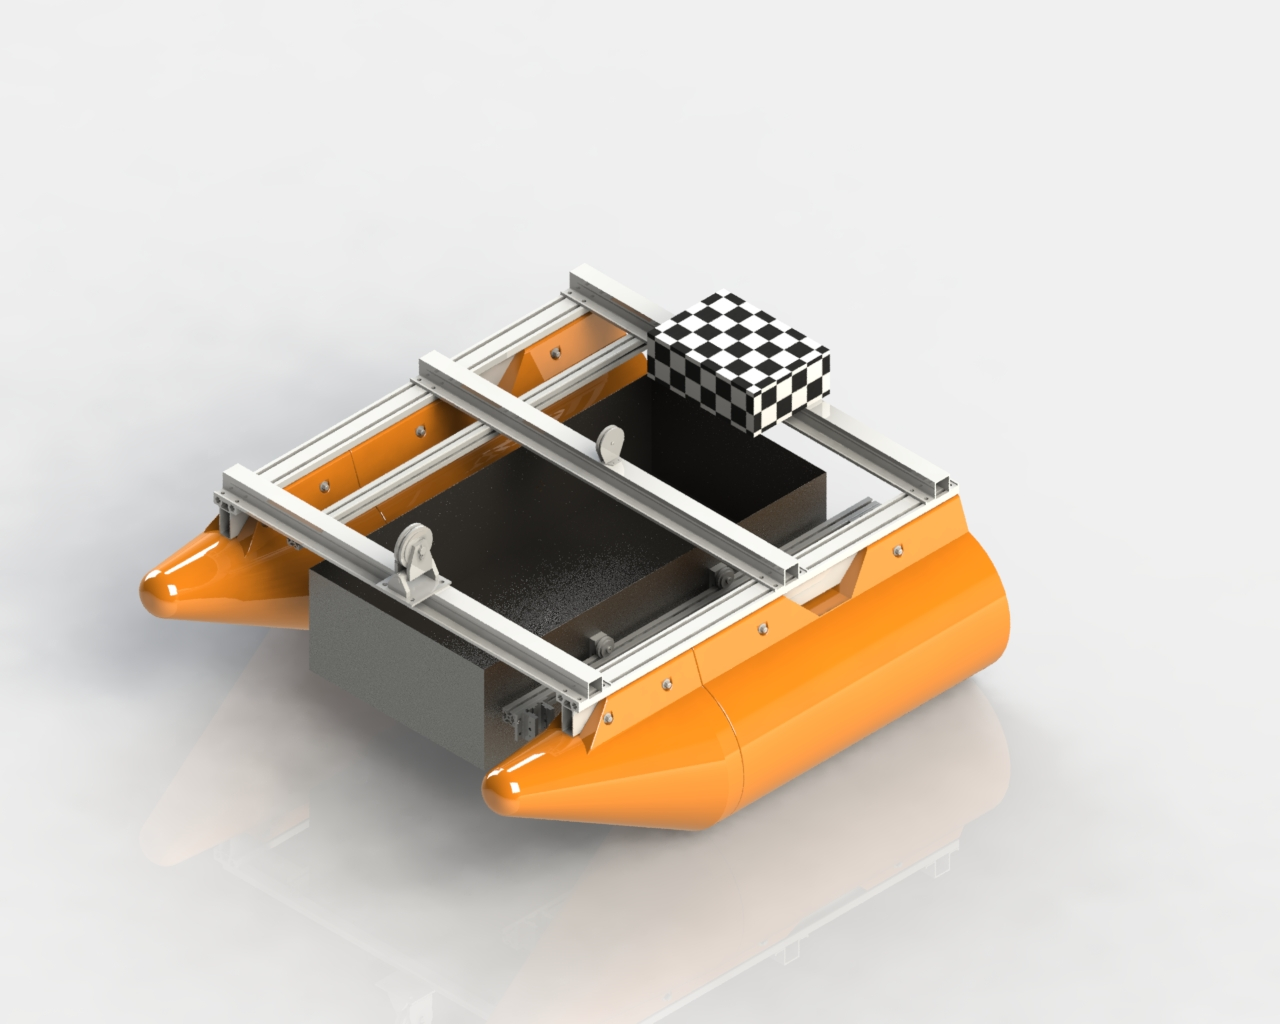
\includegraphics[width=.6\textwidth]{01rendered.png}
    \caption{Piranha rendered model, only the floats and frames are shown.}
    \label{fig:01rendered}
\end{figure}

\begin{figure}[H]
    \centering
    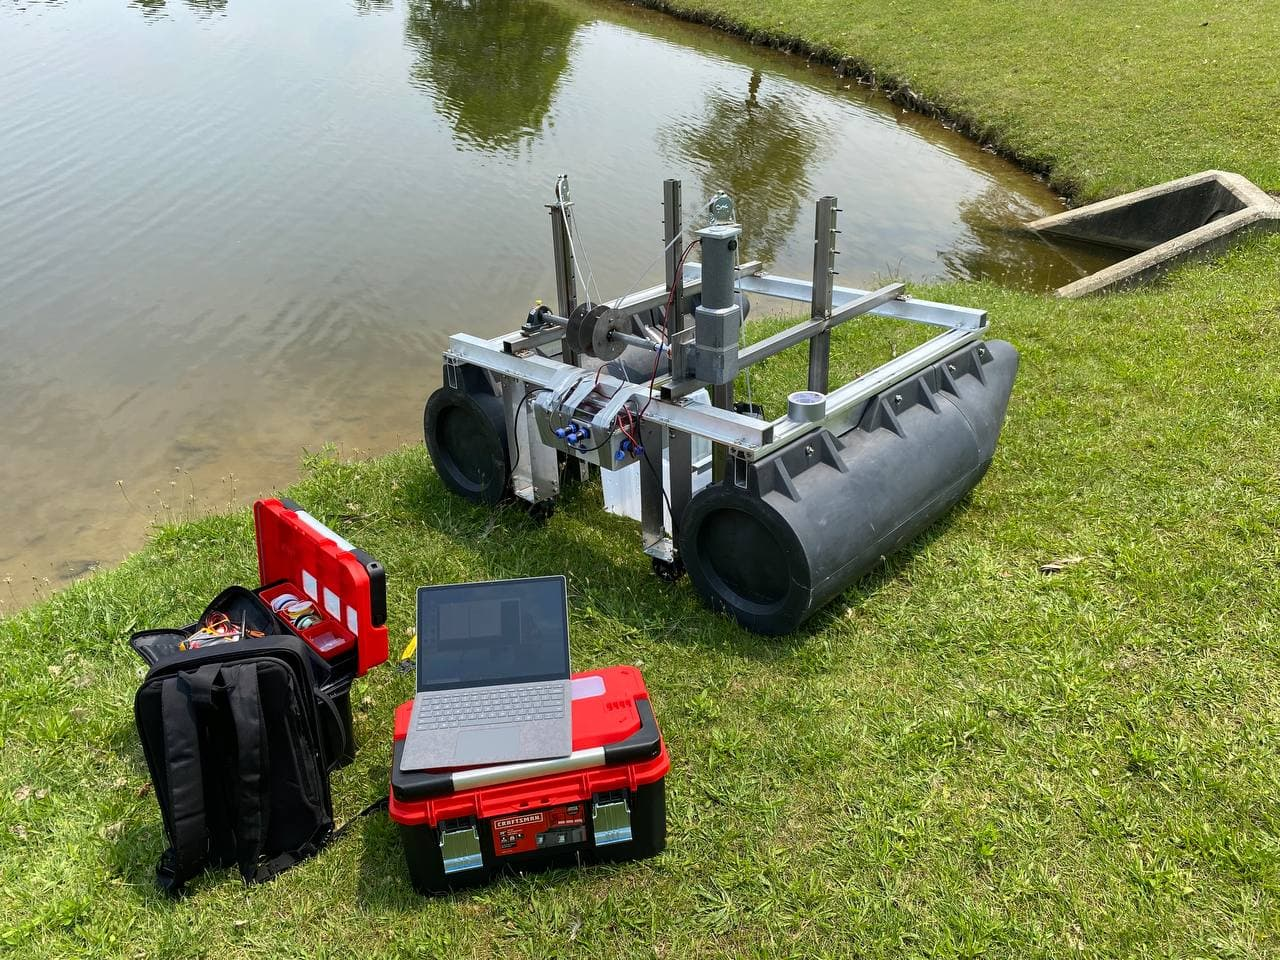
\includegraphics[width=.6\textwidth]{01piranha.jpg}
    \caption{Piranha during the forth pond test in July, 2021.}
    \label{fig:01piranha}
\end{figure}

\section{Trash collection systems}

Trash collection is the core function of Piranha. While Piranha used the simplest way to collect trash, we had several other options in the early development stage. In this section, I will introduce these different kinds of trash collection systems in the hope of inspiring more ideas from the readers.

\subsection{Venturi Pump}

The device shown in Figure \ref{fig:01air_pump} is a simplified model of a Venturi pump trash collection system. The compressed air has a leftward momentum, pushing the water to flow. As a result, the trash is captured by the water current and trapped by the net near the tube.

The advantage of this design is that there is no physical contact between the moving parts and the trash, so the chance of being stuck by the debris is relatively low. And compressed air, on the other hand, gives the boat driving power, so the thrusters are not needed anymore. These advantages are essential because driving among floating trashes with thrusters is dangerous. Ropes, plastic bags can easily get caught by the thrusters and stop the motor, which in the end leads to a complete power system failure.

However, the disadvantages of this system are that the complexity of the system and the low efficiency.  The air pump needs too much power compared with the underwater propellers. A common airboat has a 3-5 MPG fuel efficiency rating. Given by today's battery technology, it is unrealistic to drive the airboat with electricity instead of gasoline.

\begin{figure}[H]
    \centering
    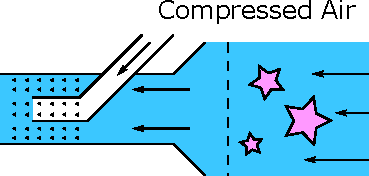
\includegraphics[width=.5\textwidth]{images/01air_pump.pdf}
    \caption{A simplified model of Venturi pump collection system. We fixed the capture net near the dotted lines. Pink stars represent the floating trashes in water. The pressure drop along the channel forces water to flow because of the Venturi effect.}
    \label{fig:01air_pump}
\end{figure}

\subsection{Conveyor}

The conveyor is the most common solution in collecting floating trashes and algae. Because if we separate the collection part from the trash container, then the trash volume depends on the container only. And the mechanical design is more straightforward compared with the Venturi pump solution. A simple combination of a passive roller and a motorized roller is enough. The conveyor-based trash collection system is shown in Figure \ref{fig:01conveyor}.

\begin{figure}[H]
    \centering
    \resizebox{.5\textwidth}{!}{\input{images/01conveyor.pdf_tex}}
    \caption{A Conveyor collection system illustration. The upper roller is motorized; meanwhile, the lower roller is passive. Pink stars and the green bucket represent the trashes to be collected and the trash container, respectively.}
    \label{fig:01conveyor}
\end{figure}

\begin{figure}[H]
    \centering
    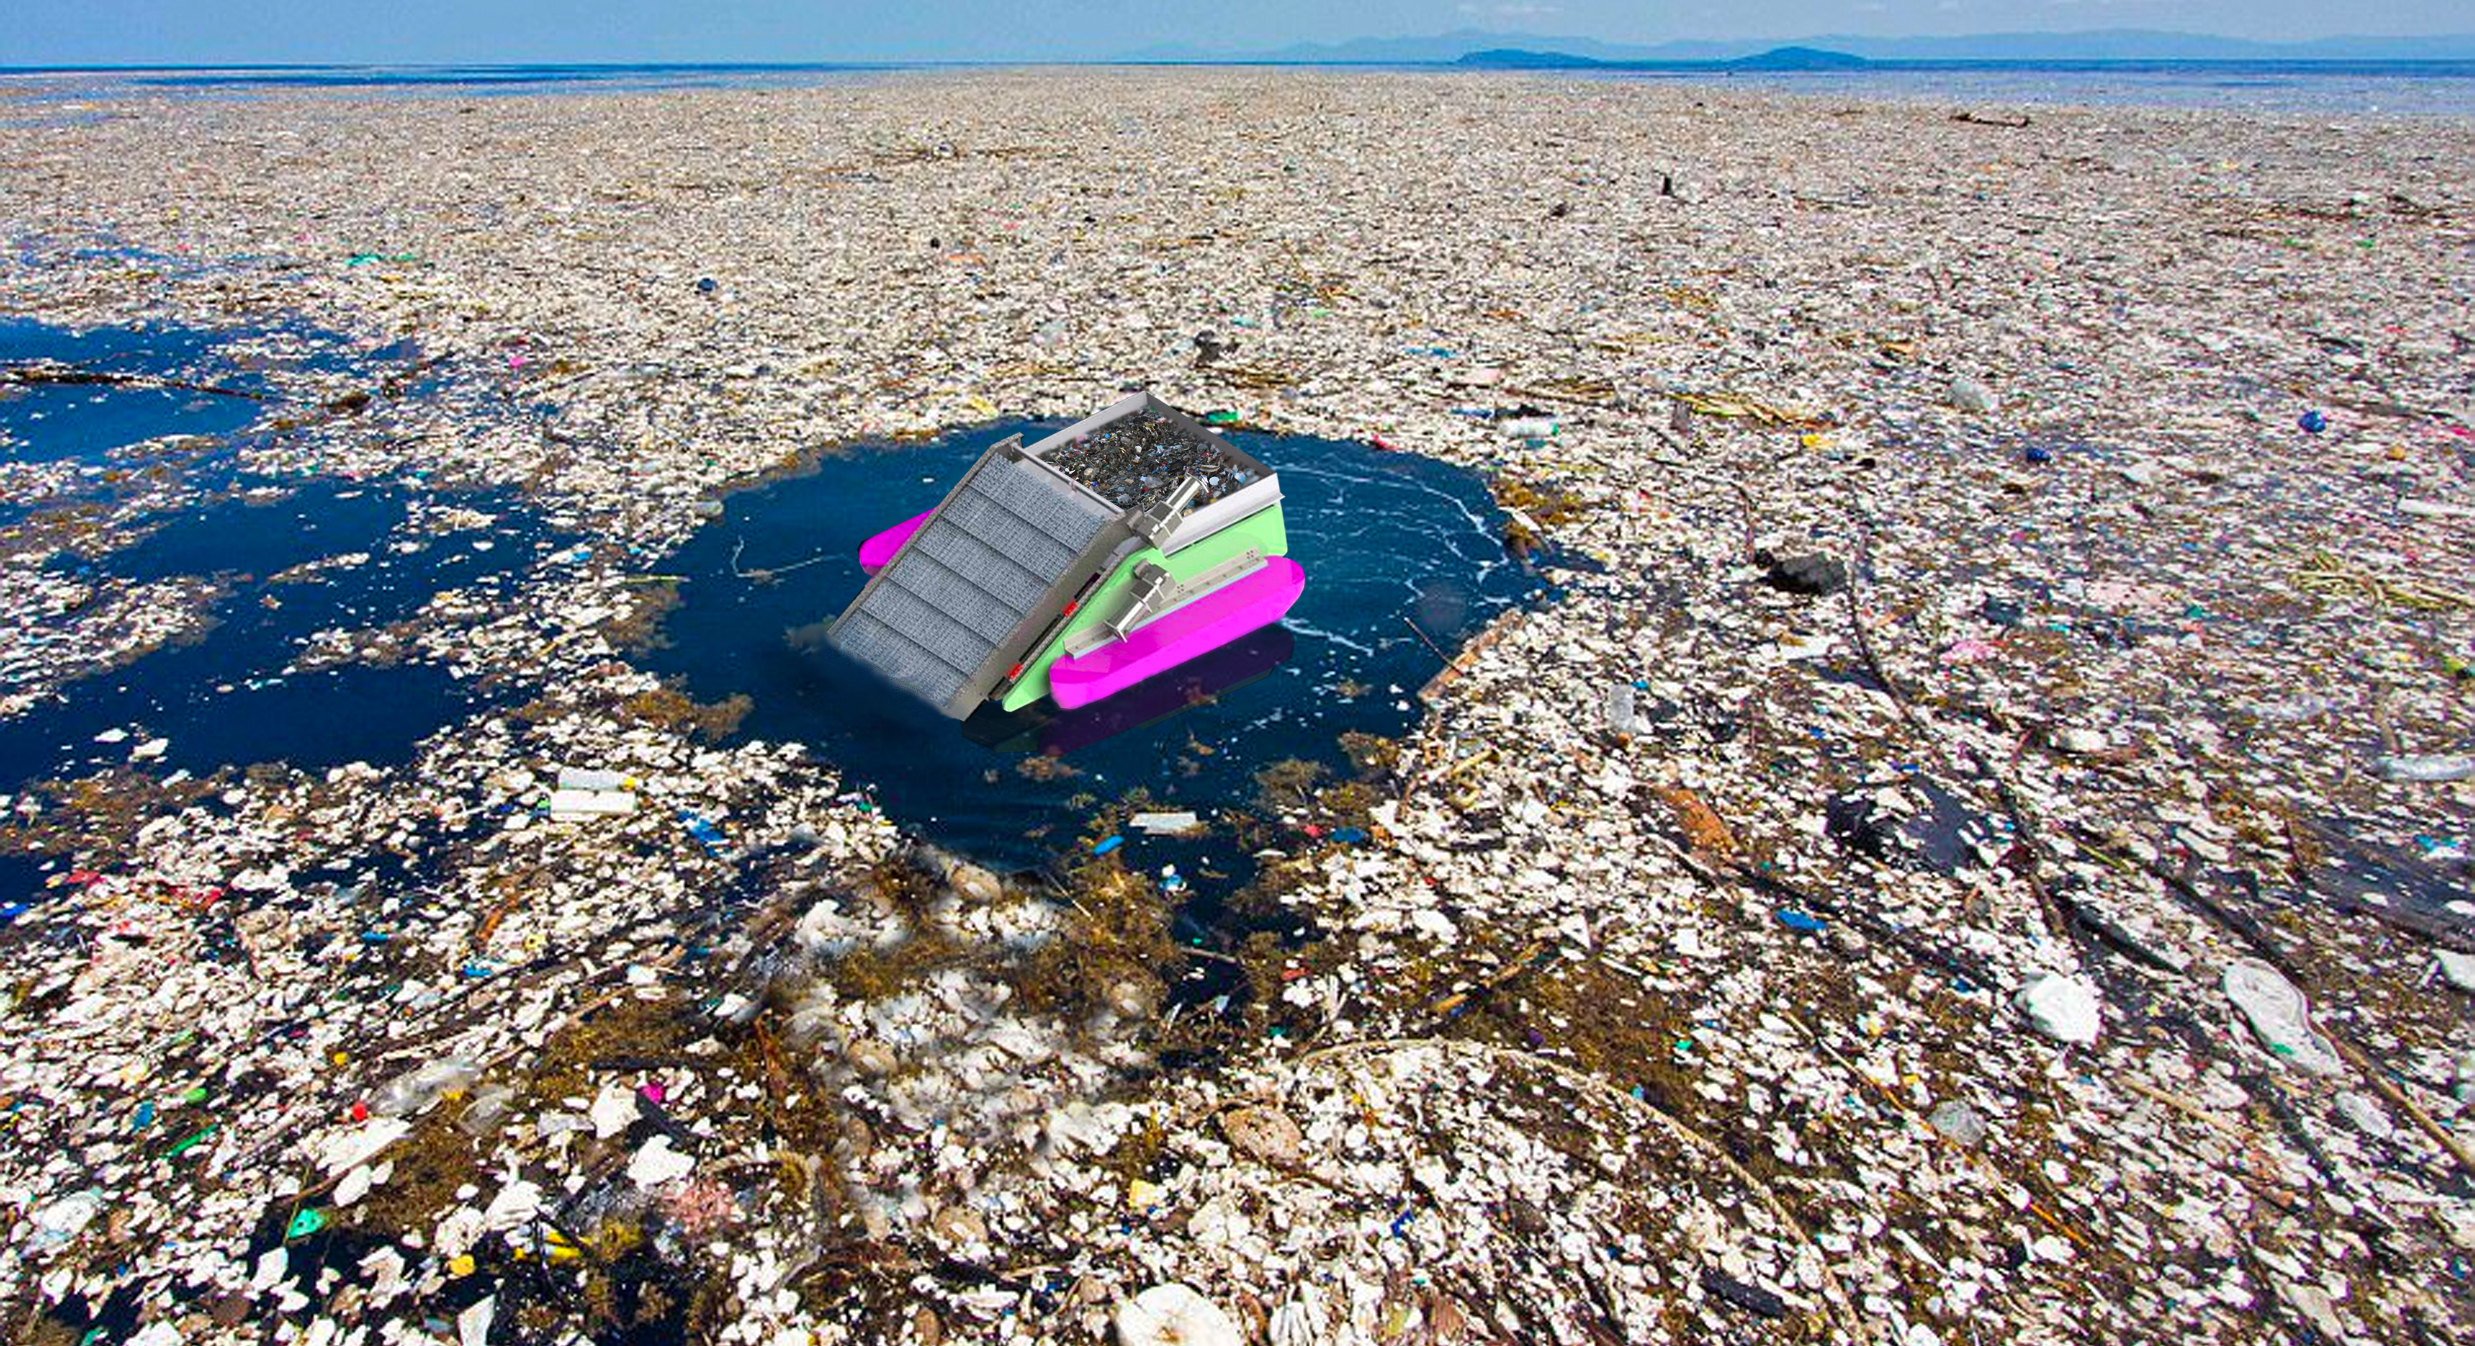
\includegraphics[width=.8\textwidth]{01orca_in_water.jpg}
    \caption{A concept model of Piranha using the conveyor collection system.}
    \label{fig:01orca_in_water}
\end{figure}

However, this configuration is usually seen on large-sized boats because there are too many moving parts, and the cost is considerably higher than other options. On Piranha, we did try the conveyor configuration as the model shown in the Figure \ref{fig:01orca_in_water}. However, due to the high cost and the difficulty in manufacturing, we decided not to adopt this design at the early development stage.

\subsection{Mesh bucket}

The collection bucket is made of meshes and allows water to go through but not trashes. This collection system is passive, meaning the boat needs to carry the bucket and drive around to collect trashes.

This solution is the simplest of all choices, and the cost is low. However, it does have several drawbacks. One of them is the capacity of the mesh bucket limits the total trash carried by Piranha in one run. Second, the bucket is submerged in water, making it very hard for workers to empty the bucket at the dumpsite. Last by most important, because the bucket does not provide any active forces on the already captured trash, there is no guarantee that the garbage will not come out of the bucket if the boat drives backward.

Piranha has a simple lever system to avoid the last two issues. The lever system illustration is shown in Figure \ref{fig:01lever-net}.

\begin{figure}[H]
    \centering
    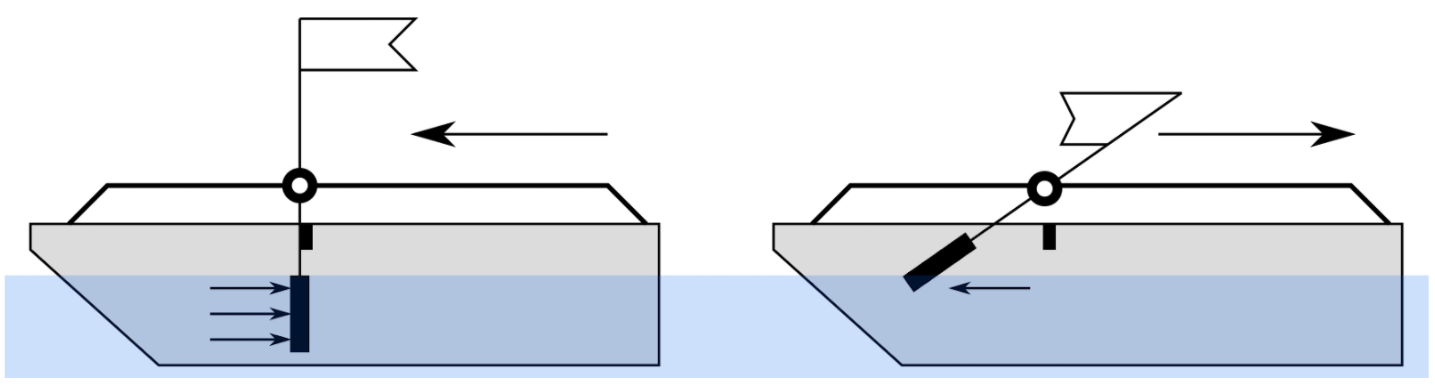
\includegraphics[width=.8\textwidth]{images/01lever-net.png}
    \caption{On the left part, the Piranha is driving forward. On the right part, Piranha is moving backward.}
    \label{fig:01lever-net}
\end{figure}

We carefully designed the lever so that it is nearly perfectly balanced in the vertical position. A minor disturbance will change the angle of the pole. As shown in the left part of the figure, if Piranha drives forward, the rod is vertical because of the water pressure on the lower part. The net's mouth opens in the vertical direction, and trash starts to flow inside the bag.

The right part shows the situation when Piranha drives backward. The lower part starts moving up due to the water pressure. The mouth of the net leaves the water so that the trash cannot escape. In such a way, the lever automatically "seals" the net when the Piranha starts driving backward or the water current is faster than the boat and is about to bring out the trash. 

\section{Similar Robots}

Some other robots can do a similar job as Piranha at the time when we designed Piranha. Almost all of them have one of the configurations mentioned in the previous section. However, they vary in some subtle details when it comes to the goals and technologies behind them.

\subsection{WasteShark}

Sponsored by the Robotics Innovation Center in Germany and the European Union, WasteShark has a very similar design to Piranha. They claimed WasteShark could carry 350-kilogram trash in one run. It also has a special navigation algorithm to allow the robot to return to the dock once the bucket is full. Several water quality sensors on the boat can detect the water quality data, including pH, ORP, conductivity, dissolved oxygen, turbidity, ammonium, chloride, nitrate, salinity, mV, ORP, TDS, resistivity level, and send them back to the data center\cite{SCHMALTZ2020106067}.

\subsection{Clearbot}

Clearbot shown in Figure \ref{fig:01clearbot} is an intelligent robot designed by a company in Hong Kong. It is very similar to Piranha, except it used a conveyor instead of a mesh bucket. According to the description provided on their website, Clearbot has a self-driving function and a computer and camera to identify the type of garbage and upload the data to a cloud-based platform.

Clearbot's primary function is collecting trash from the water, cleaning the rivers and oceans globally. Besides that, it can also identify a wide range of waste and material types to help the recycling companies to classify the trashes. According to the recent updates, the developers of Clearbot are working on the swarm algorithm for the robot.

\begin{figure}[H]
    \centering
    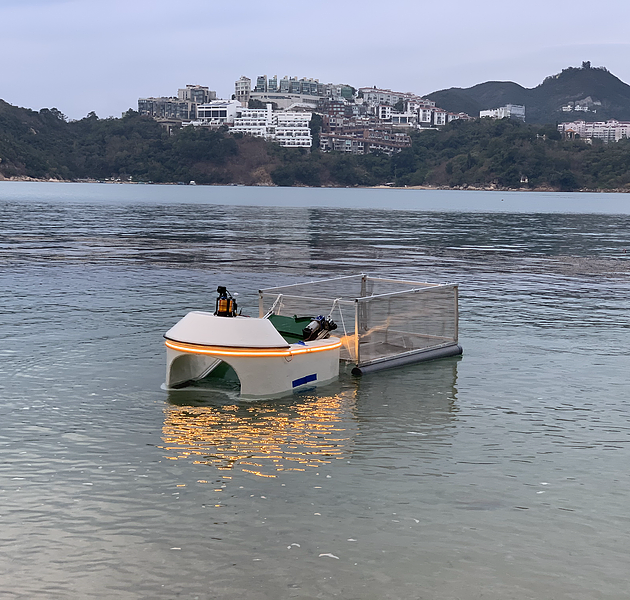
\includegraphics[width=.6\textwidth]{01clearbot.png}
    \caption{Clearbot.}
    \label{fig:01clearbot}
\end{figure}

\chapter{Mechanical Design}

This chapter includes the mechanical details of Piranha. To begin with, Piranha is a twin-body pontoon boat. It has two floats on the left and right sides to support its weight. The only motorized parts on Piranha are the left and right thrusters installed at the rear. In other words, Piranha is a skid steering boat. Both thrusters provide the driving forces forward or backward, allowing Piranha to move forward and back. The difference between the thruster outputs generates the torque required for steering.

Readers can find The overall design of Piranha in Figure \ref{fig:02rendered_all}.

\begin{figure}[H]
    \centering
    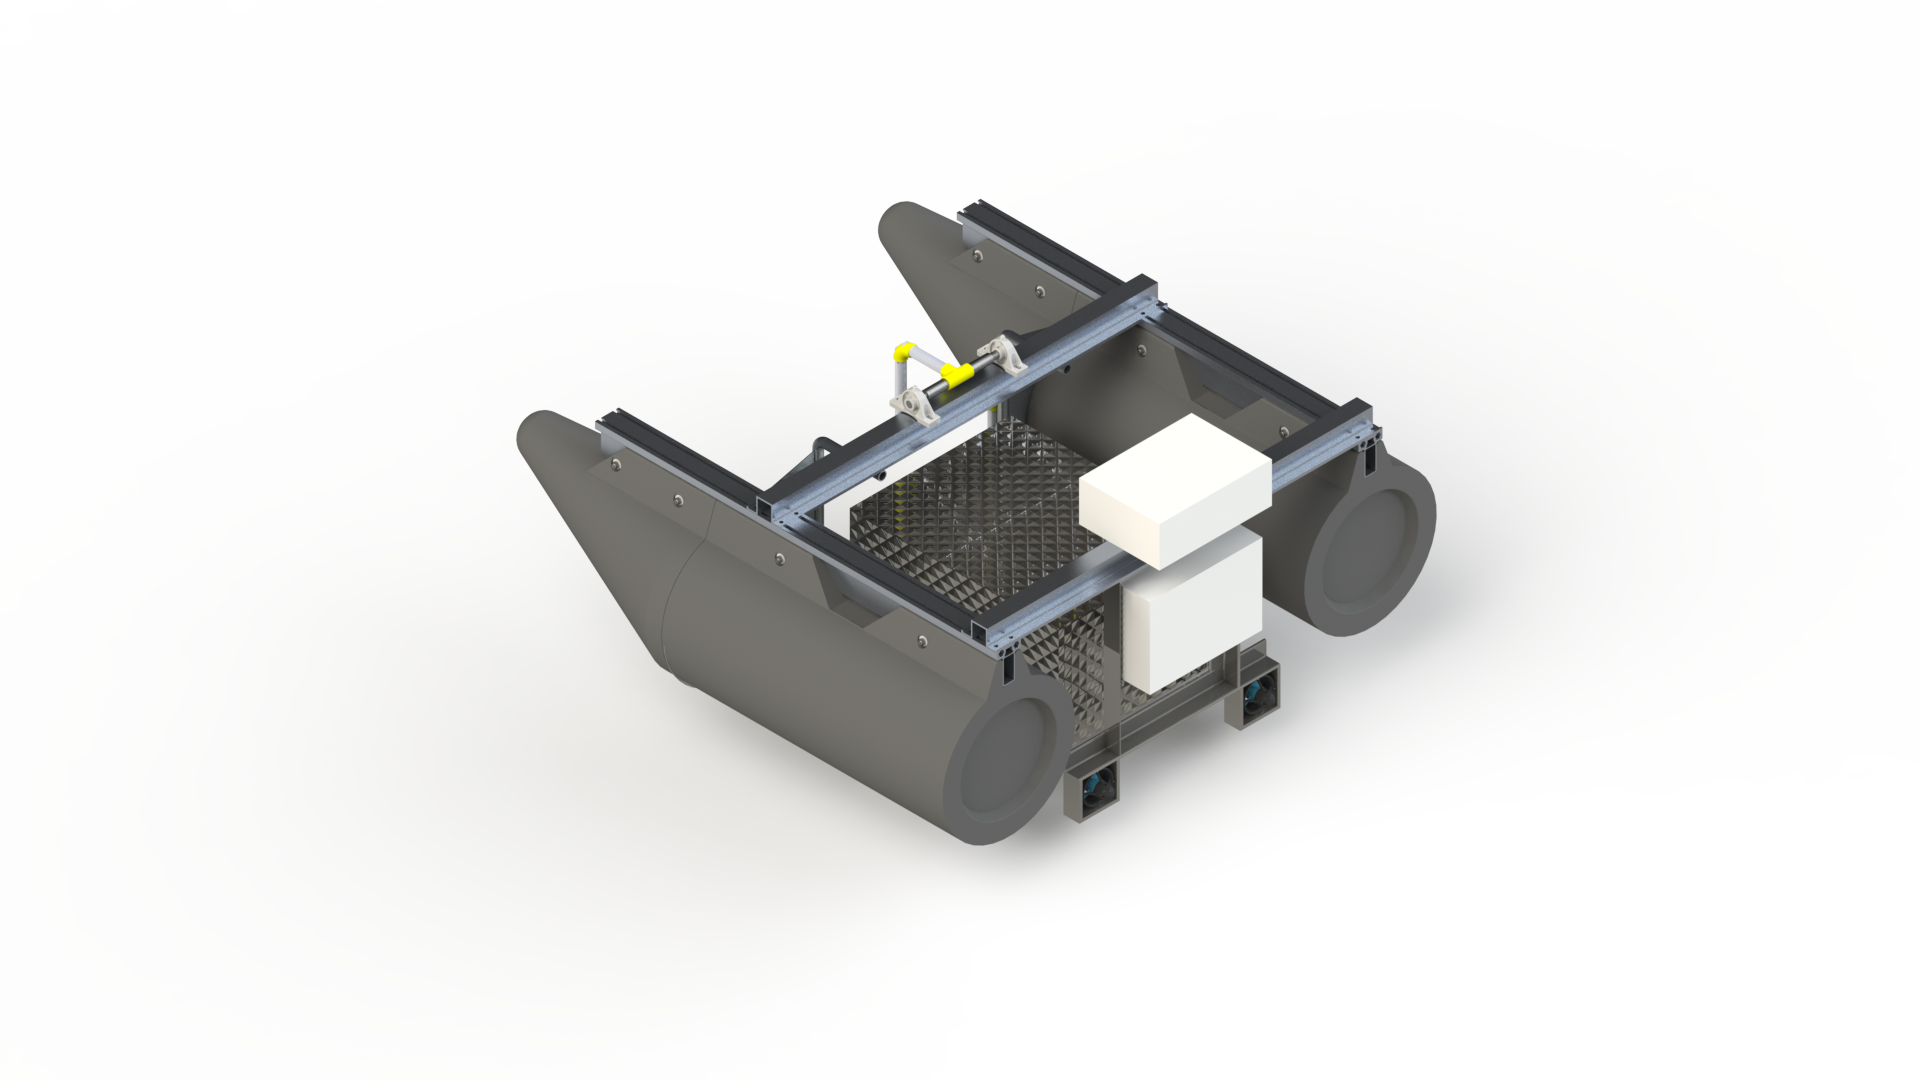
\includegraphics[width=.8\textwidth]{images/02orca-back.png}
    \caption{A rendered model of Piranha. The white blocks represent the electrical system box and the battery pack.}
    \label{fig:02rendered_all}
\end{figure}

\section{Floats}

Piranha's floating parts, including the connection frame, are sold by \textit{Silver Lake Fabrication LLC D.B.A Tiny Pontoon Boats}. The floats are made of High-Density Poly Ethylene (HDPE) with closed-cell urethane foam filling. The connection frame is made of aluminum.

The specifications of the pontoon nose part in Figure \ref{fig:02nose-cone}, can be found in Table \ref{table:02nose-cone}.

\begin{figure}[H]
    \centering
    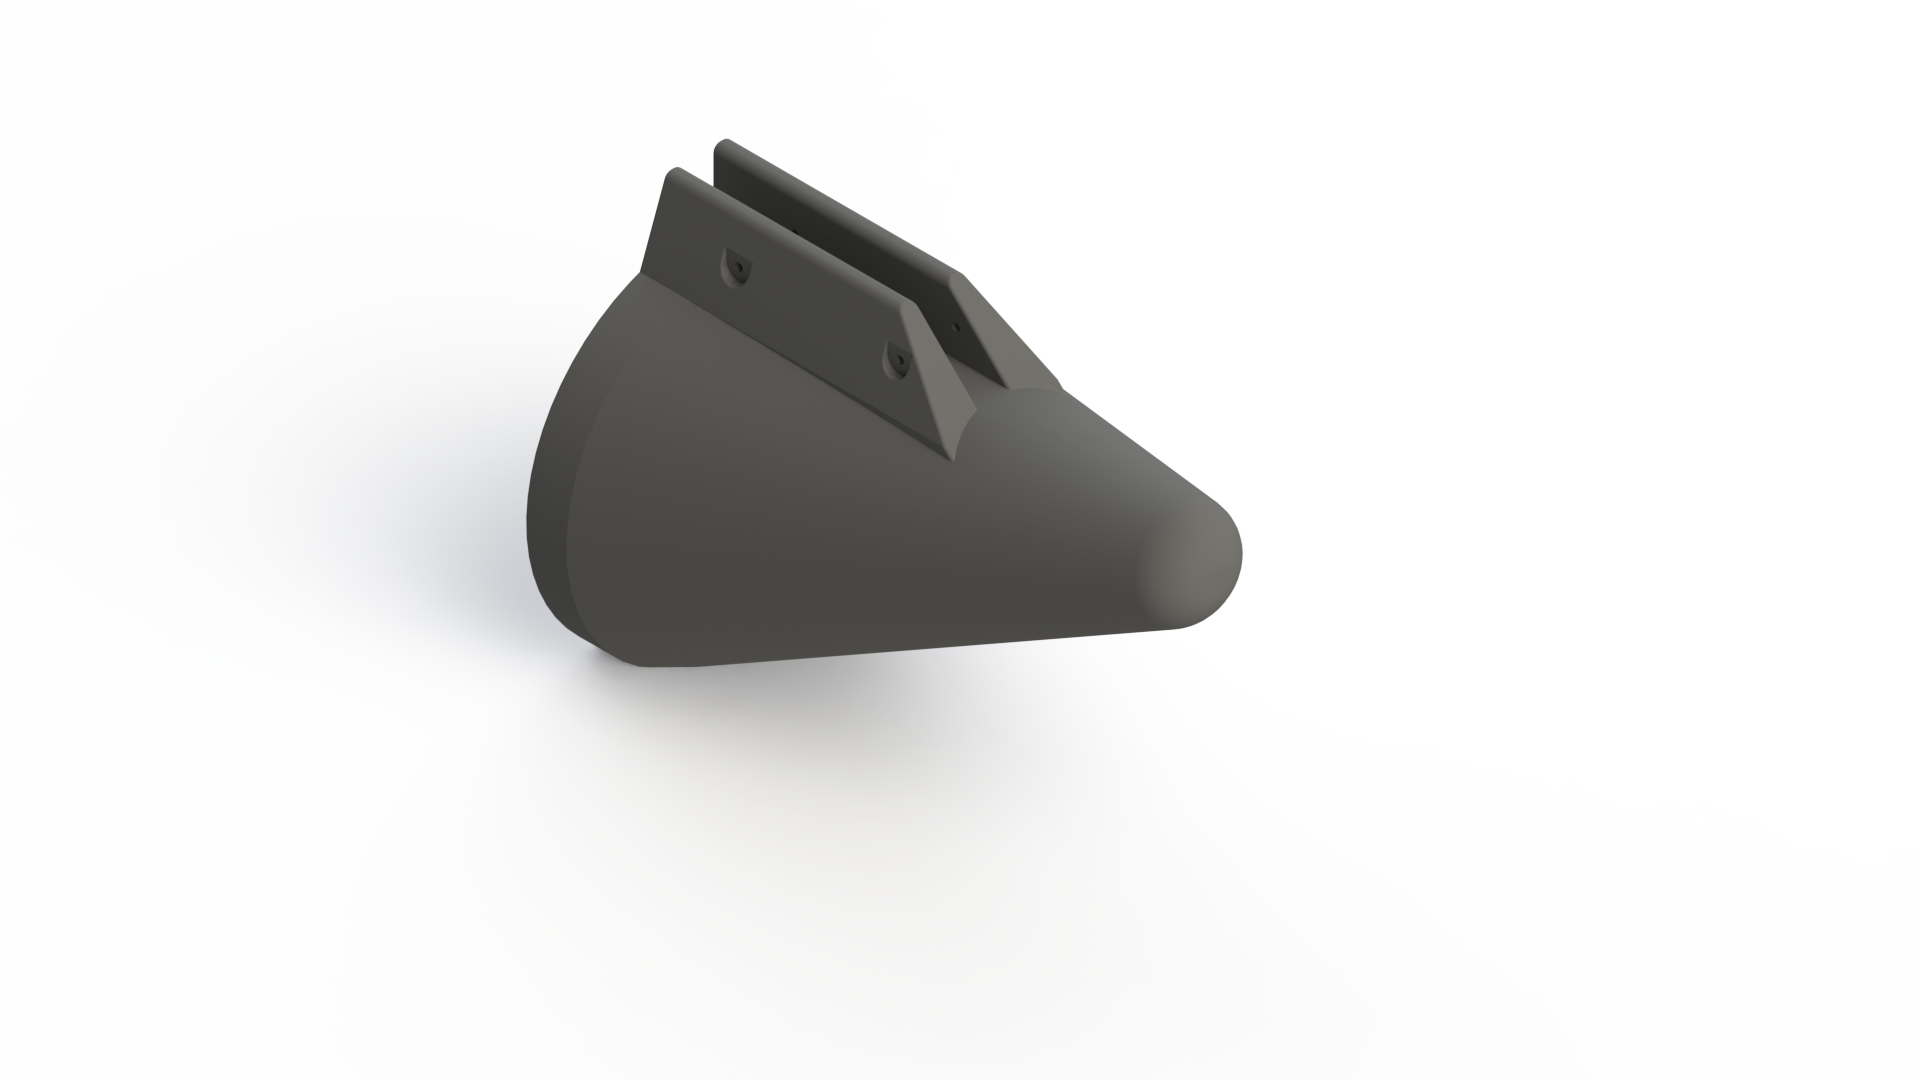
\includegraphics[width=.6\textwidth]{images/02nose-cone.png}
    \caption{Pontoon nose cone.}
    \label{fig:02nose-cone}
\end{figure}

\begin{table}[H]
\caption{Specifications of 17" Diameter Pontoon Nose Cones} % title of Table
\centering % used for centering table
\renewcommand{\arraystretch}{0.8}
\begin{tabular}{l l}
\hline
\textbf{Characteristics} & \textbf{Rating} \\ 
%heading
\hline % inserts single horizontal line
Float width & 16.5 inches \\
Float length & 25 inches \\
Weight & 14 lbs \\
Rated capacity & 45 lbs \\
\hline
\end{tabular}
\label{table:02nose-cone} % is used to refer this table in the text
\end{table}

The specifications of the pontoon straight part in Figure \ref{fig:02pontoon-body}, can be found in Table \ref{table:02pontoon-body}.

\begin{figure}[H]
    \centering
    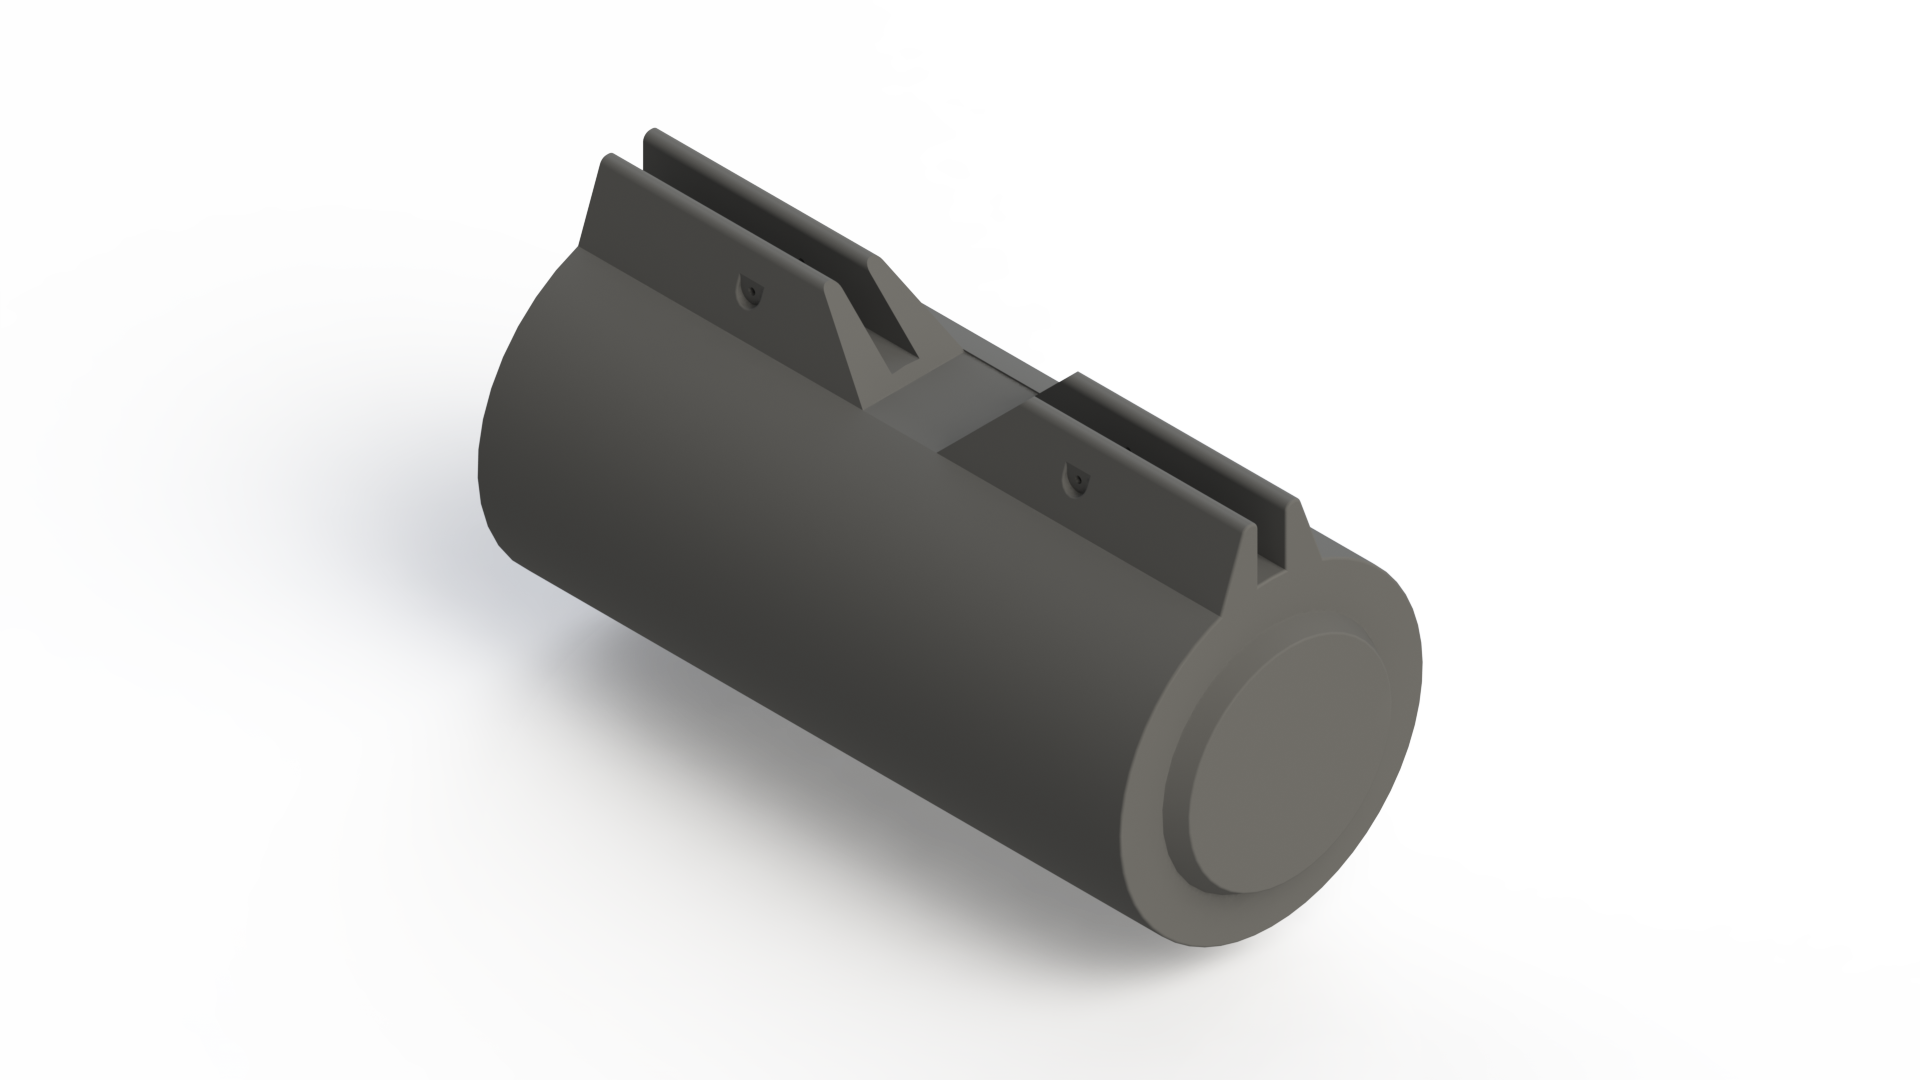
\includegraphics[width=.8\textwidth]{images/02pontoon-body.png}
    \caption{Pontoon body.}
    \label{fig:02pontoon-body}
\end{figure}

\begin{table}[H]
\caption{Specifications of 17" Diameter Pontoon Nose Cones} % title of Table
\centering % used for centering table
\renewcommand{\arraystretch}{0.8}
\begin{tabular}{l l}
\hline
\textbf{Characteristics} & \textbf{Rating} \\ 
%heading
\hline % inserts single horizontal line
Float width & 16.5 inches \\
Float length & 36 inches \\
Weight & 23 lbs \\
Rated capacity & 130 lbs \\
\hline
\end{tabular}
\label{table:02pontoon-body} % is used to refer this table in the text
\end{table}

\subsection{Float Assembly}

Piranha connects the float parts by the aluminum frame, shown in Figure \ref{fig:02orca-frame}. The screws and nuts are made of stainless steel to prevent corrosion.

\begin{figure}[H]
    \centering
    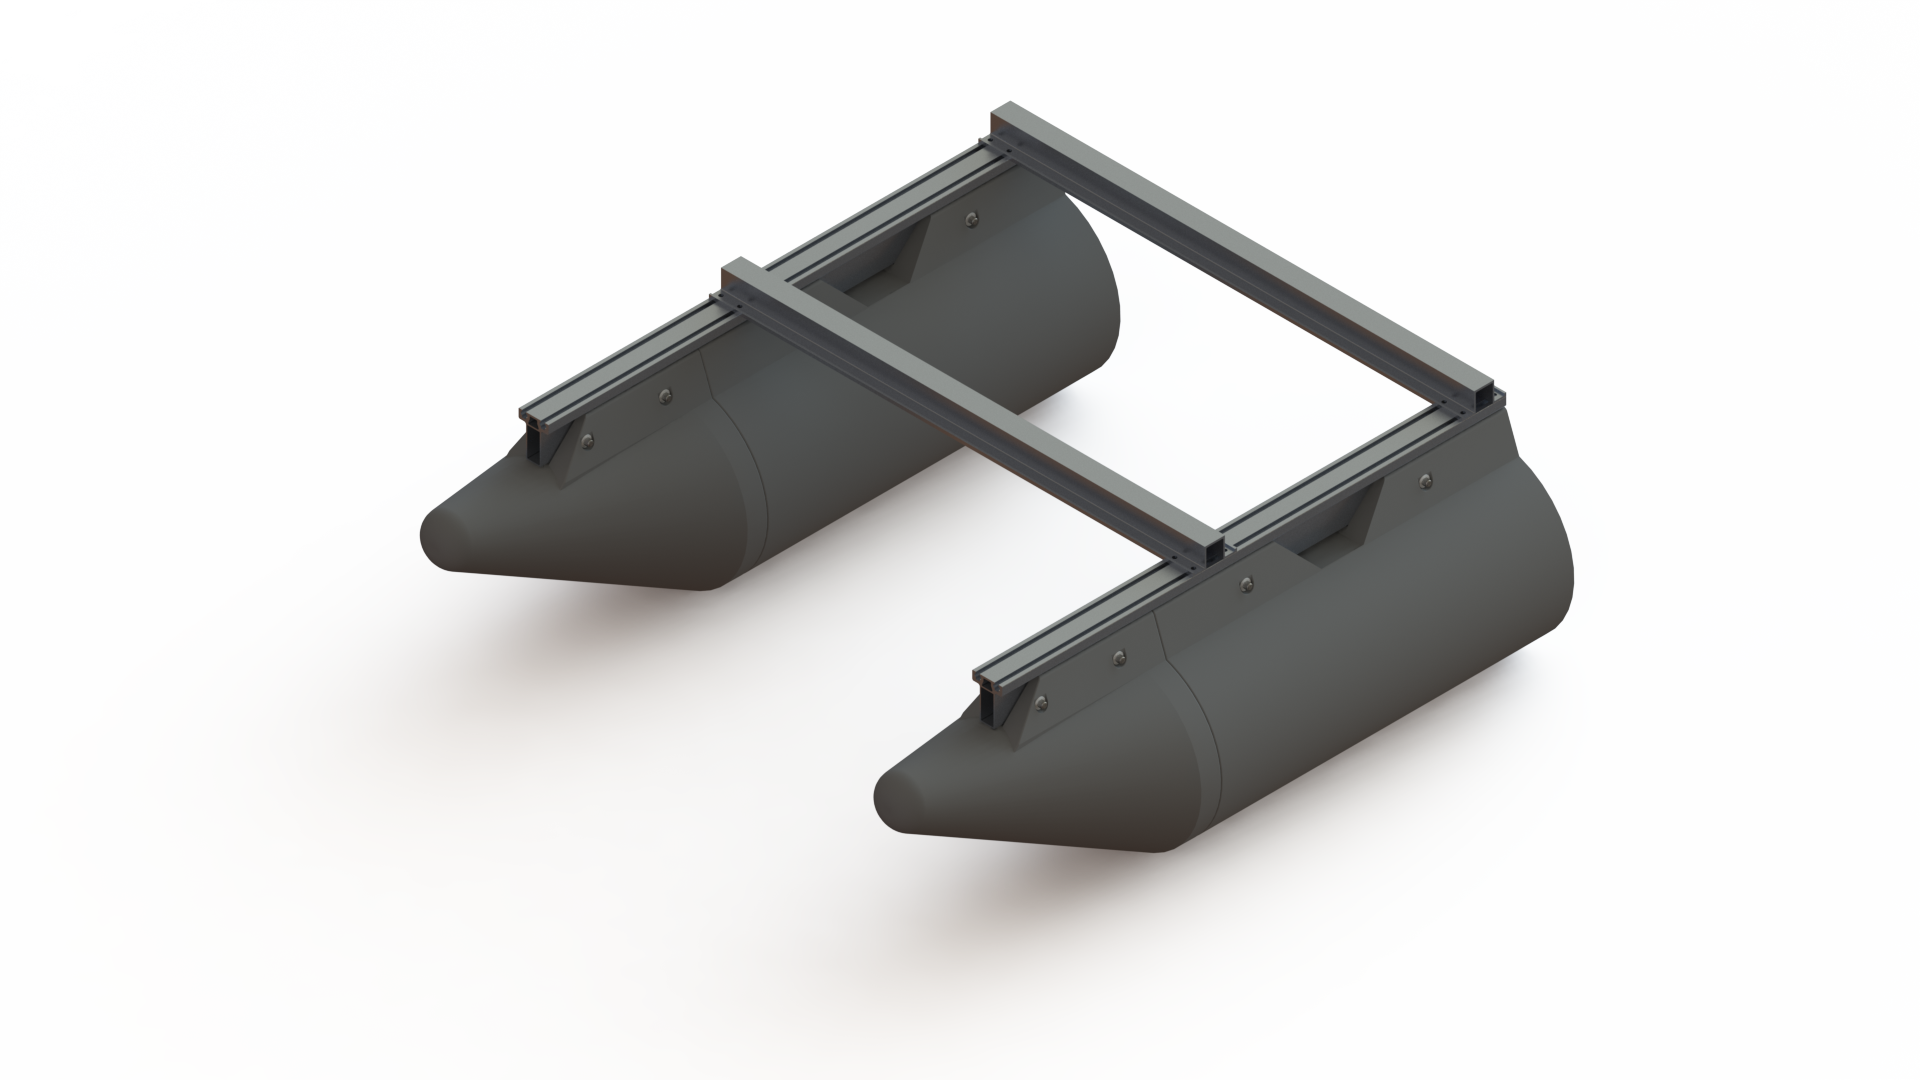
\includegraphics[width=.8\textwidth]{images/02orca-frame.png}
    \caption{The overall float assembly.}
    \label{fig:02orca-frame}
\end{figure}

\section{Thrusters}

Piranha has two thrusters installed at the rear. The thruster model is BlueRobotics T200 Thruster. Its mechanical drawing can be found in Figure \ref{fig:02t200-3d}, \ref{fig:02t200-back}. Table \ref{table:02thruster} lists the specifications for them.

\begin{table}[H]
\caption{Physical Specifications of the BlueRobotics T200 Thruster} % title of Table
\centering % used for centering table
\renewcommand{\arraystretch}{0.8}
\begin{tabular}{l l}
\hline
\textbf{Characteristics} & \textbf{Rating} \\ 
%heading
\hline % inserts single horizontal line
Width & 113 mm \\
Length & 100 mm \\
Weight & 344 g \\
Propeller Diameter & 76 mm \\
\hline
\end{tabular}
\label{table:02thruster} % is used to refer this table in the text
\end{table}

\begin{figure}[H]
    \centering
    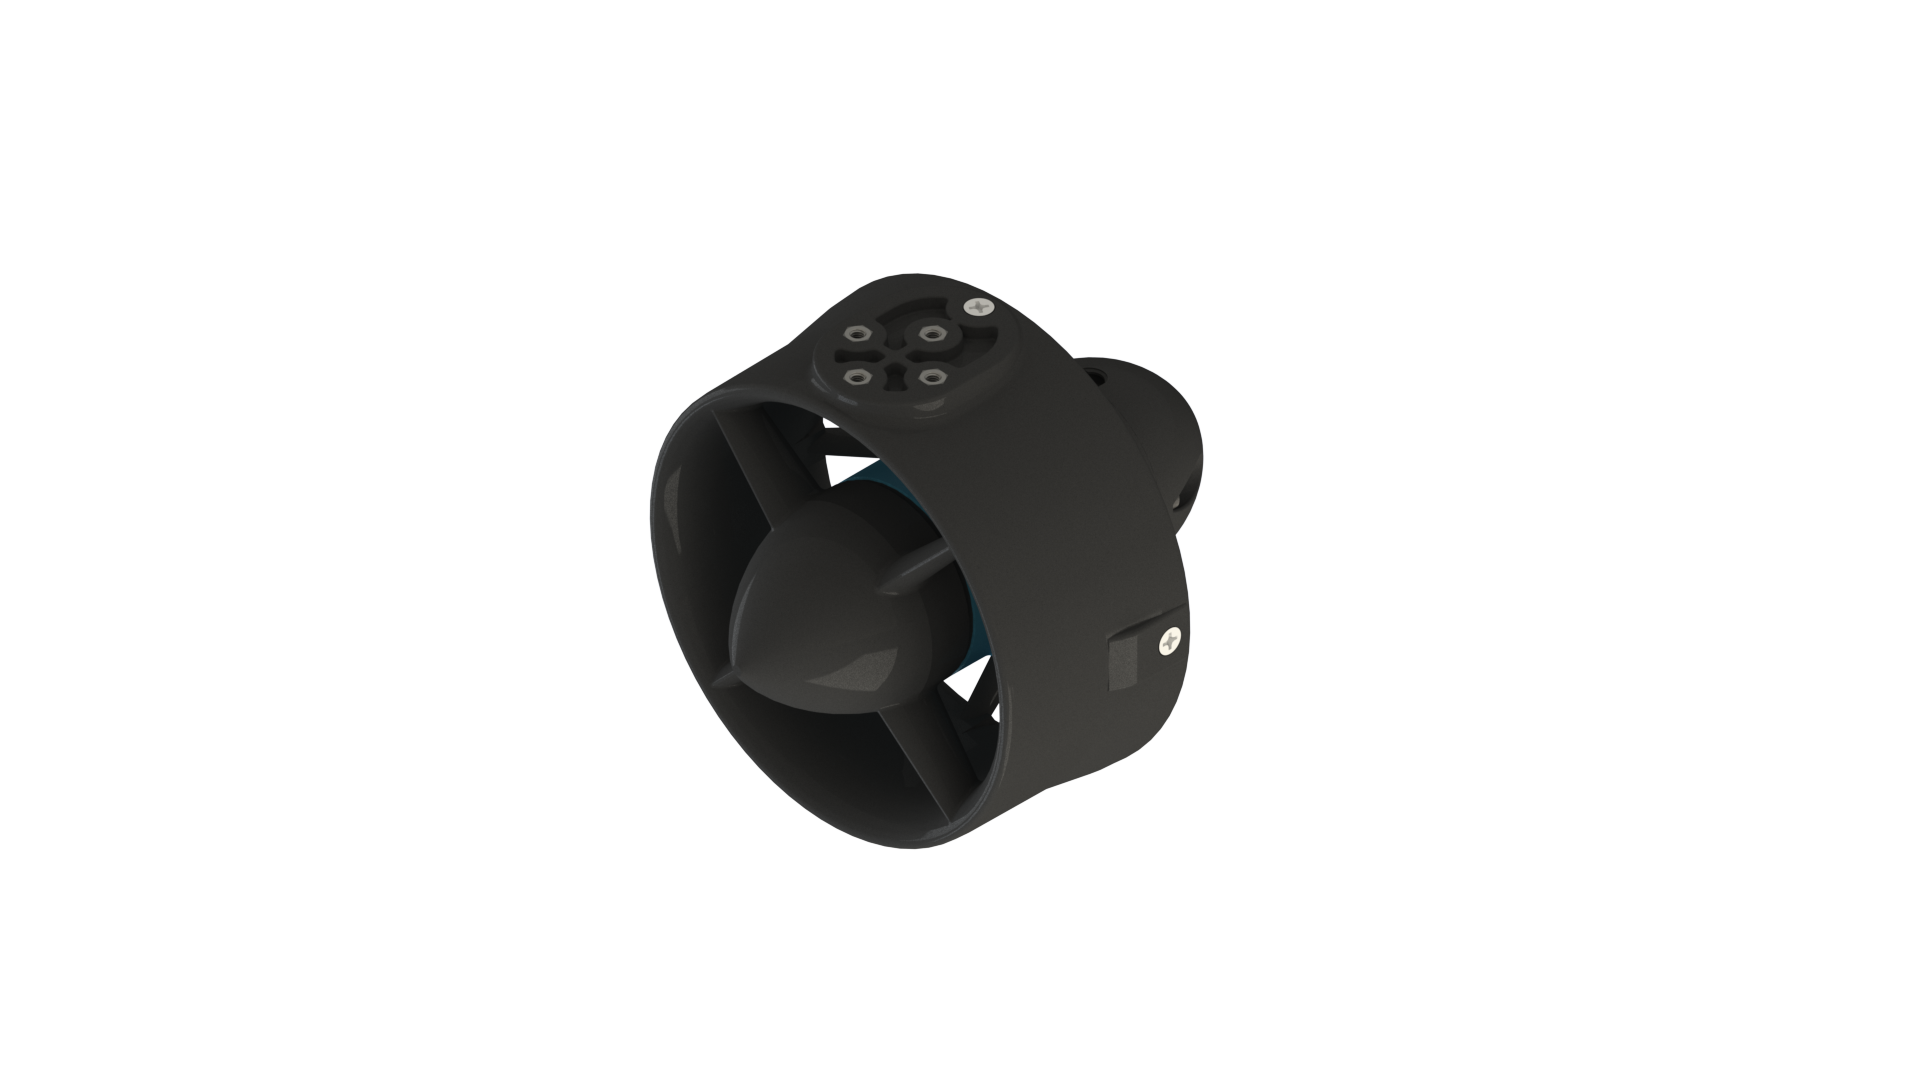
\includegraphics[width=.8\textwidth]{images/02t200-thruster.png}
    \caption{BlueRobotics T200 Thruster (Isometric View).}
    \label{fig:02t200-3d}
\end{figure}

\begin{figure}[H]
    \centering
    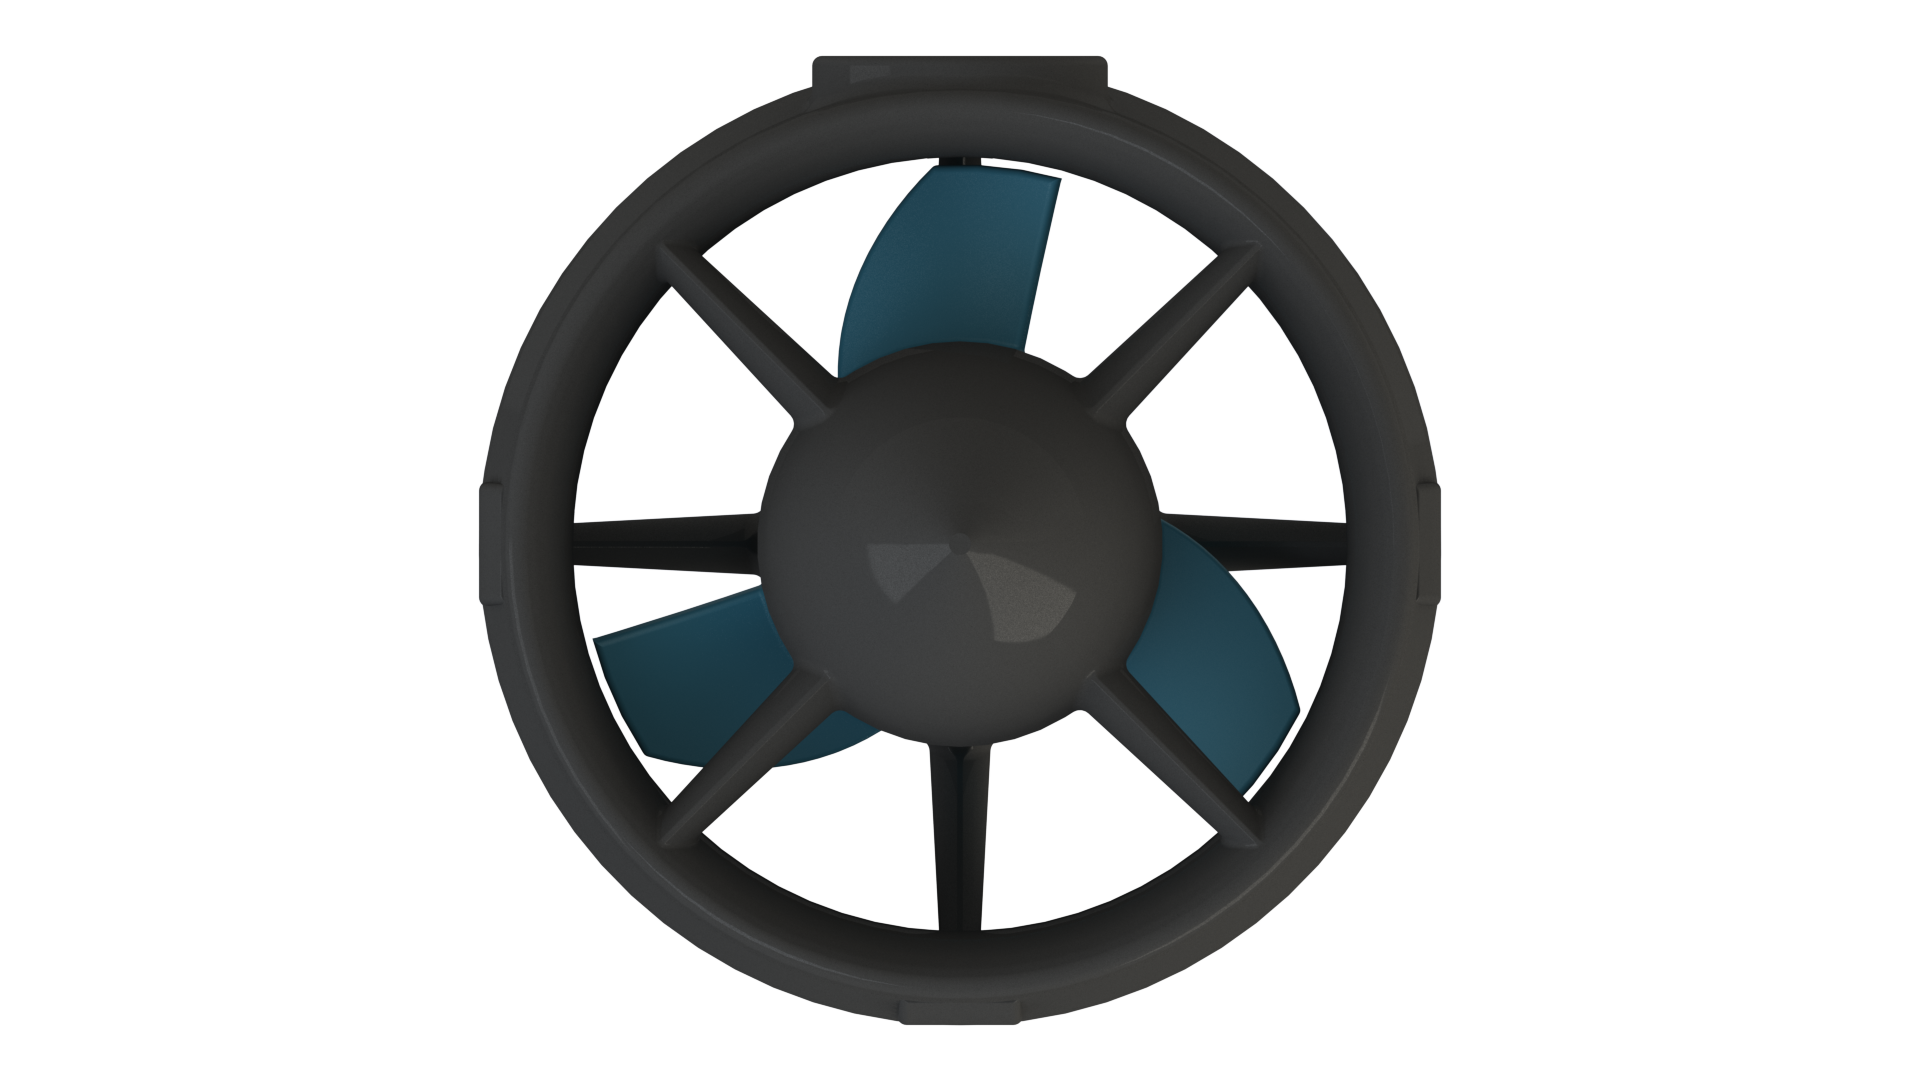
\includegraphics[width=.8\textwidth]{images/02t200-thruster-back.png}
    \caption{BlueRobotics T200 Thruster (Back View).}
    \label{fig:02t200-back}
\end{figure}

\subsection{Thruster Locations}

Figure \ref{fig:02orca-thruster} shows the location of the two thrusters.

\begin{figure}[H]
    \centering
    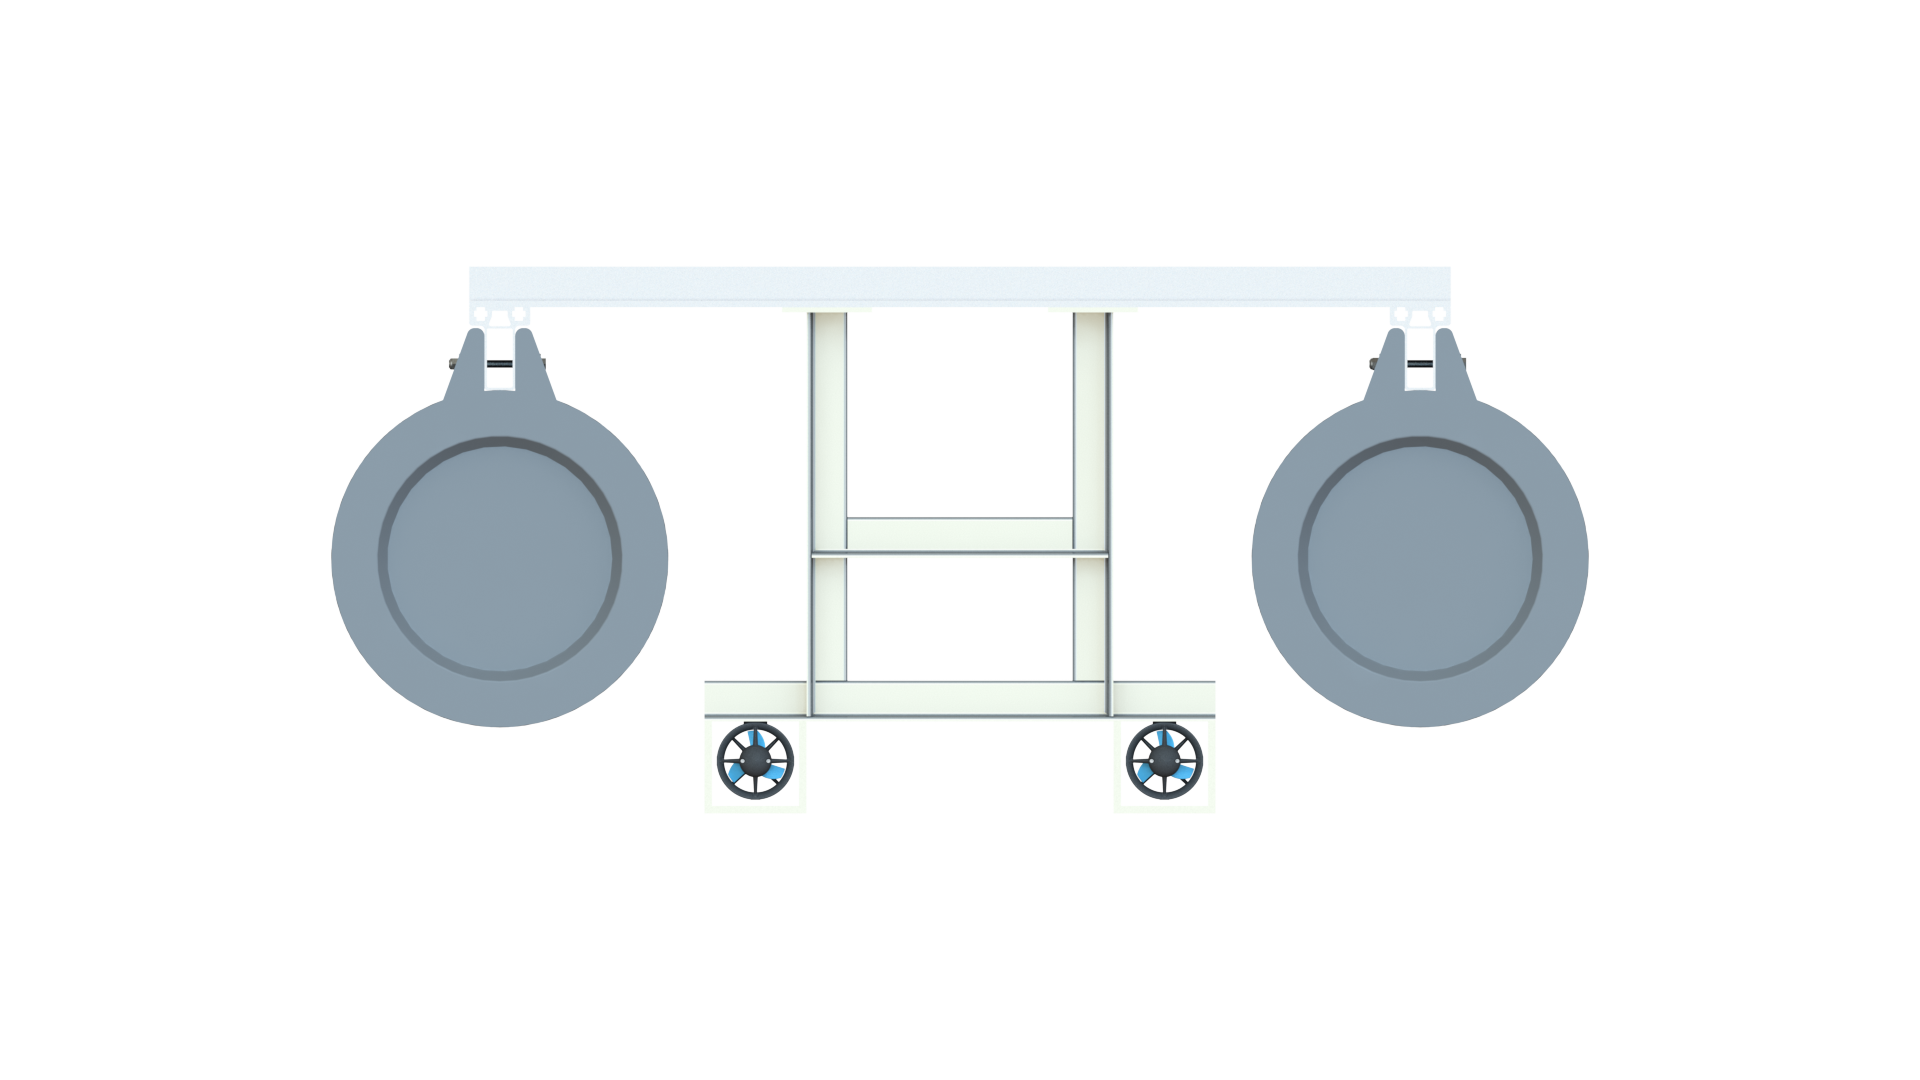
\includegraphics[width=.8\textwidth]{images/02orca-thruster.png}
    \caption{Two thrusters are installed at the rear of Piranha.}
    \label{fig:02orca-thruster}
\end{figure}

\chapter{Electrical System}

Readers can find a simplified schematic of Piranha's electrical system in Figure \ref{fig:03overview}. Figure \ref{fig:03test-bench} shows the real-world test bench. 

\begin{figure}[H]
    \centering
    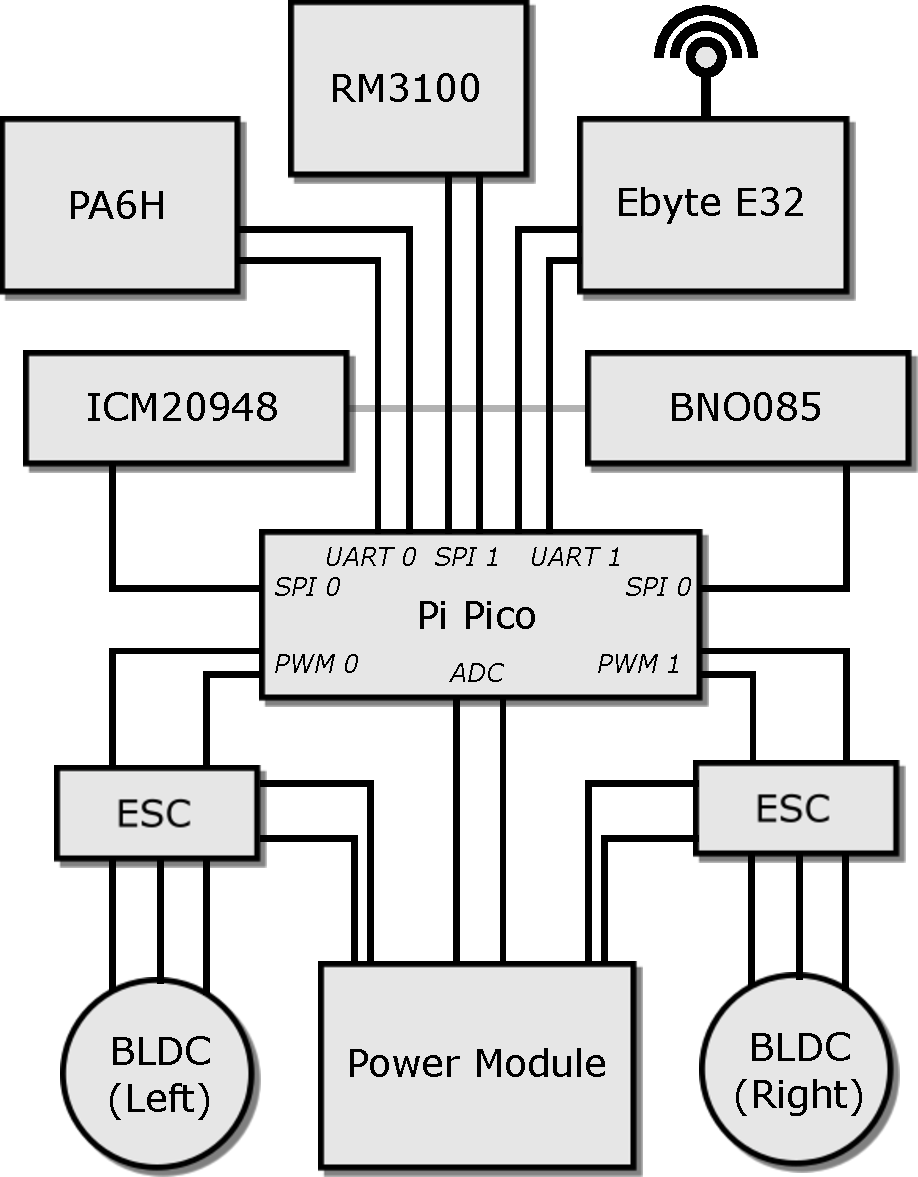
\includegraphics[width=.5\textwidth]{03overview.pdf}
    \caption{The electrical system overview.}
    \label{fig:03overview}
\end{figure}

\begin{figure}[H]
    \centering
    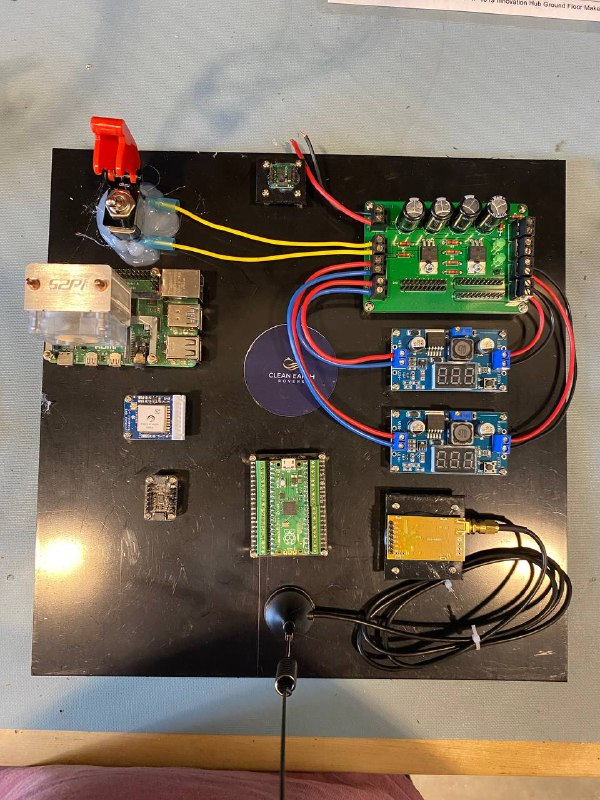
\includegraphics[width=.8\textwidth]{images/03test-bench.jpeg}
    \caption{The figure shows Piranha's test module we built in 1819 Innovation Hub for testing the software functions and electrical design.}
    \label{fig:03test-bench}
\end{figure}

\section{Power Module}

We customized the power module on Piranha to distribute the necessary electrical power to every modules module, including the electrical speed controllers, the Pi Pico, sensors, etc. The board is designed by KiCad and manufactured by JLCPCB. Since the power module carries more than 40-ampere current in the working condition, we covered the PCB with an extra copper layer made by the laser cutter.

The power module also contains several physical switches, including a master switch, two emergency stop switches, and a voltage measurement point for maintenance usage. These switches control the power output to the two thrusters by controlling the gate voltages of two TK4R3E06PL MOSFETs. Table \ref{table:03mosfet} lists its specifications.

The schematic and the rendered 3D model of the Piranha's power module are provided in Figure \ref{fig:03power} and Figure \ref{fig:03shutdown3d}. A PCB prototype board is shown in Figure \ref{fig:03power-pcb}, the electrical components are not soldered yet.

\begin{figure}[H]
    \centering
    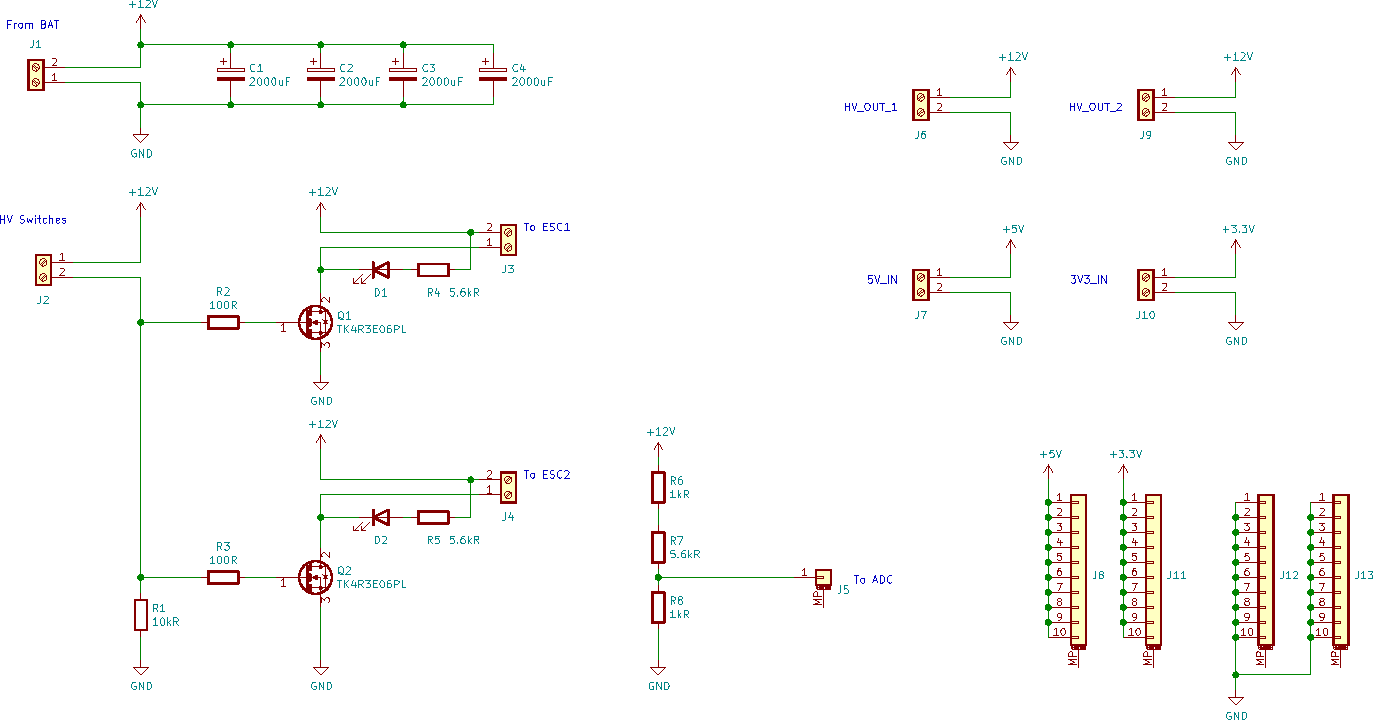
\includegraphics[width=.9\textwidth]{images/03shutdown-sch-no-title.pdf}
    \caption{The overall schematic of the power module.}
    \label{fig:03power}
\end{figure}

\begin{figure}[H]
    \centering
    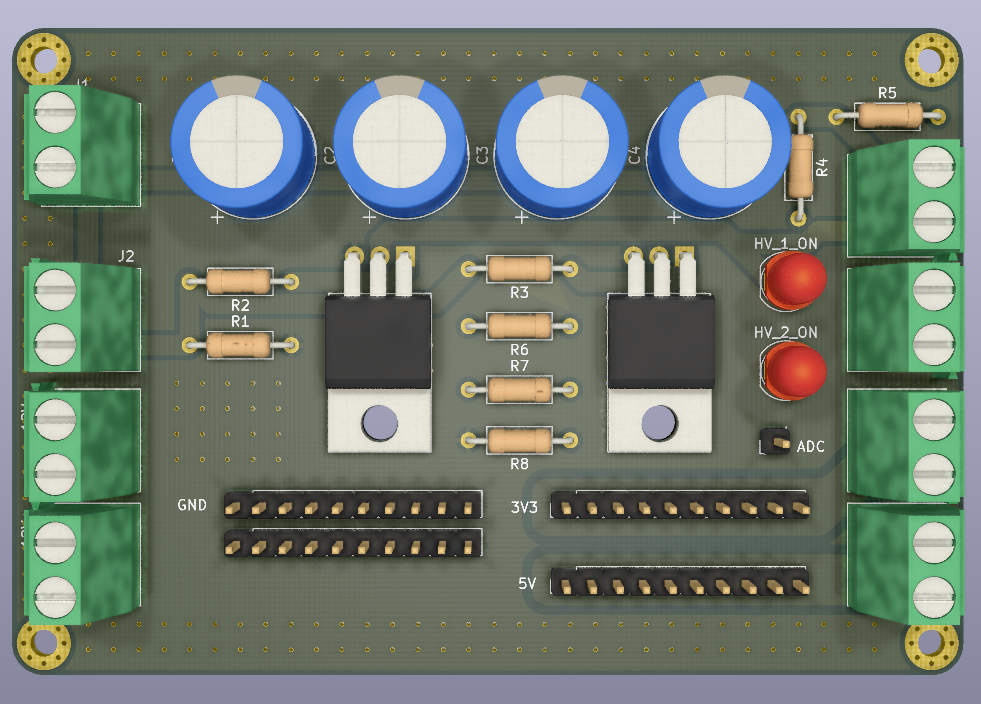
\includegraphics[width=.8\textwidth]{03shutdown3d.png}
    \caption{Power module rendered 3D view in KiCad.}
    \label{fig:03shutdown3d}
\end{figure}

\begin{figure}[H]
    \centering
    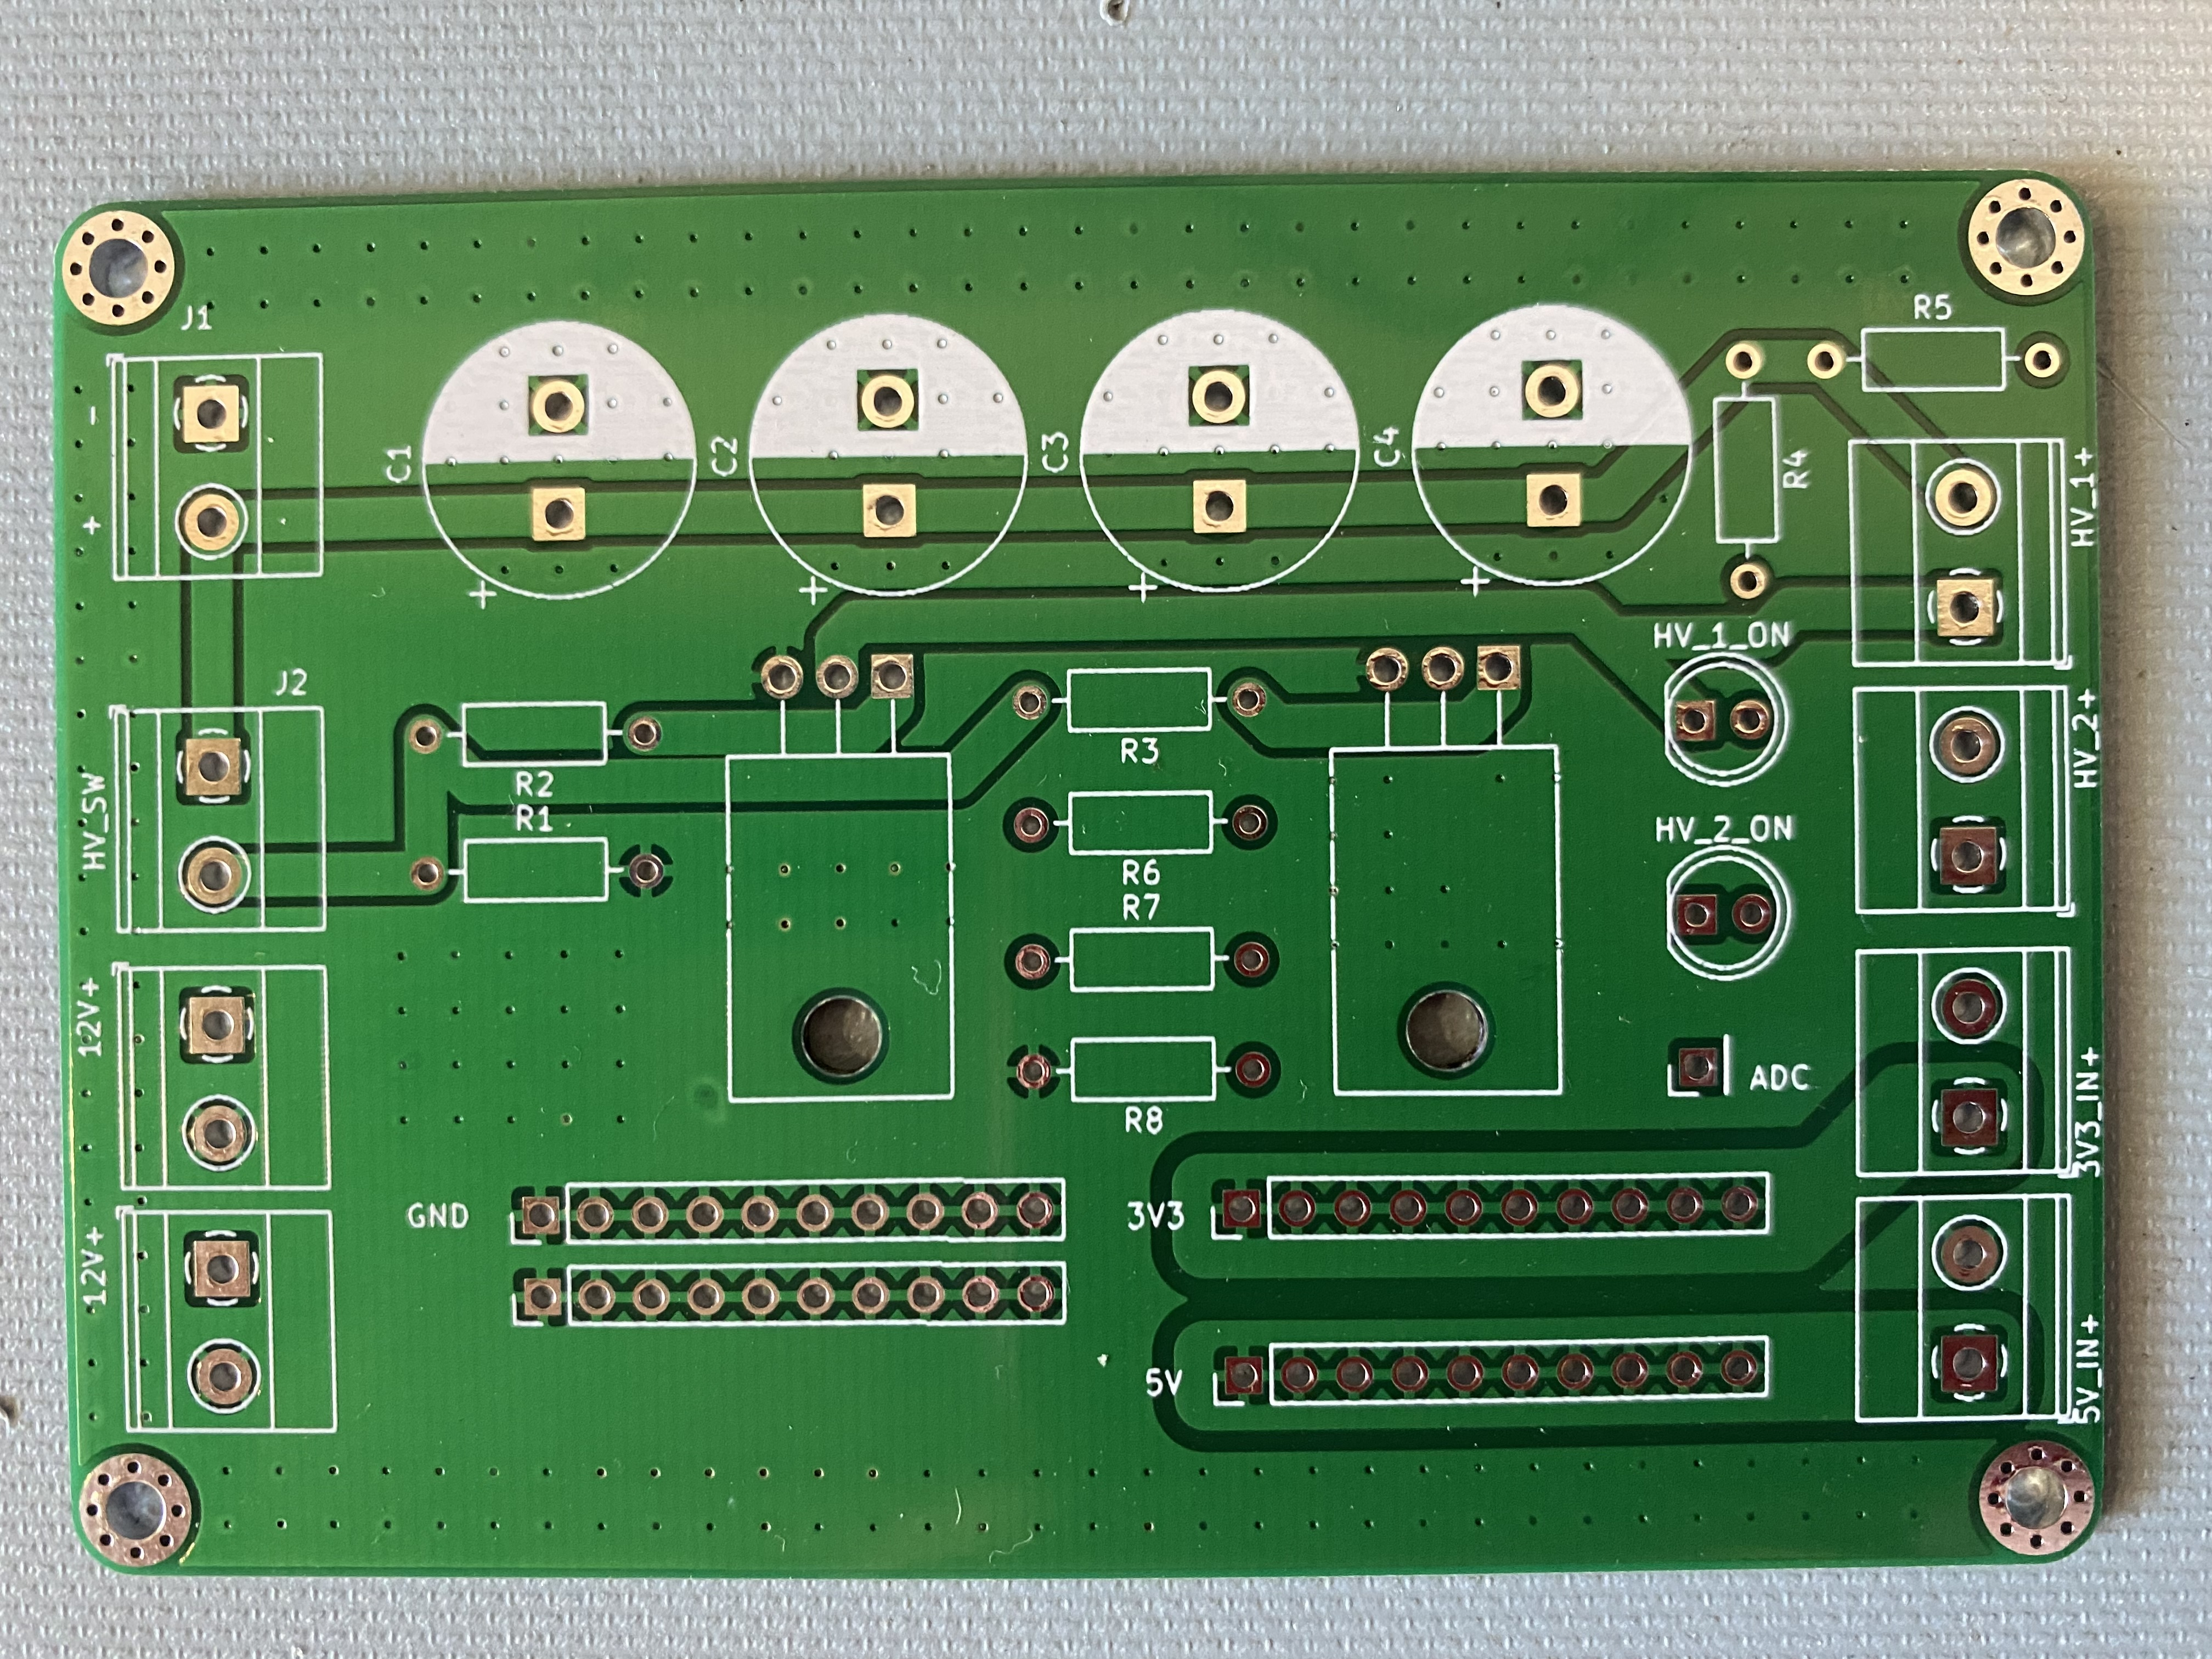
\includegraphics[width=.8\textwidth]{images/03power-module-pcb.JPG}
    \caption{The PCB prototype for the power board manufactured by JLCPCB.}
    \label{fig:03power-pcb}
\end{figure}

Table \ref{table:03powerboard} lists the Piranha's power board specification.

\begin{table}[ht]
\caption{Technical Specifications of the Power Board} % title of Table
\centering % used for centering table
\renewcommand{\arraystretch}{0.8}
\begin{tabular}{l l} % centered columns (4 columns)
\hline
\textbf{Characteristics} & \textbf{Rating} \\ [0.5ex] % inserts table
%heading
\hline % inserts single horizontal line
Maximum input voltage  & $25\ V$ \\
Maximum main output current & $2\times 80\ A$ \\
Maximum working temperature & $125\degree\ C$ \\
Maximum $3.3V$ output current & $3\ A$ \\
Maximum $5V$ output current & $3\ A$ \\
\hline %inserts single line
\end{tabular}
\label{table:03powerboard} % is used to refer this table in the text
\end{table}

Please know that this table only describes the capability of the power board itself. It does not reflect the whole system limitation. For example, the maximum current consumed by a thruster is only $24\ A$.

\subsection{MOSFET}

The power module has two Toshiba TK4R3E06PL MOSFETs as the primary relays. You can find part of its technical specifications in Table \ref{table:03mosfet}. These MOSFETs carry the whole current for the two electrical speed controllers. The external physical switches directly control the voltage on the gates. For safety reasons, no software logic is behind the power control system.

\begin{table}[ht]
\caption{Technical Specifications of TOSHIBA TK4R3E06PL (part)} % title of Table
\centering % used for centering table
\renewcommand{\arraystretch}{0.8}
\begin{tabular}{l c l} % centered columns (4 columns)
\hline
\textbf{Characteristics} & \textbf{Symbol} & \textbf{Rating} \\
%heading
\hline % inserts single horizontal line
Maximum drain-source voltage & $V_{DSS}$ & $60\ V$ \\
Maximum gate-source voltage & $V_{GSS}$ & $20\ V$ \\
Maximum drain current (DC) & $I_D$ & $80\ A$ \\
Maximum channel temperature & $T_{ch}$ & $175\ \degree C$ \\
Channel-to-case thermal resistance (T=$25\ \degree C$) & $R_{th(ch-c)}$  & 1.72\ \degree C/W  \\
Drain-source on-resistance at $V_{GS}=10\ V, I_D = 34\ A$ & $R_{DS(ON)}$ & $3.3{\rm m}\Omega$ (Typical) \\
\hline %inserts single line
\end{tabular}
\label{table:03mosfet} % is used to refer this table in the text
\end{table}

MOSFETs, compared with regular mechanical relays, have huge advantages over the whole life cycle \cite{TK4R3E06PL}. However, due to the characteristics of the PN junction, we need to do some calculations to ensure that, under full workload, the thermal rise of the MOSFETs is within the operational range. 

\subsection{Thermal Estimation}

Because one MOSFET controls only one thruster, the maximum load for each MOSFET approximately equals the full power of the thruster. We ignored the other power consumers like Pi Pico and ESCs since their power ratings are only a few milliwatts. The heat dissipation of the MOSFETs under the maximum workload ($24\ A$), according to Table \ref{table:03mosfet}, can be calculated through Ohm's Law:

\begin{equation}
    P_w=I^2 R_{ds(on)}=24\ A^2 \times 3.3\ {\rm m}\Omega=1.9008\ W
\end{equation}

Given the room temperature $25\degree C$, the maximum junction temperature under full workload is:

\begin{equation}
    T_j=T_r+P_w R_{th(ch-c)}=25\degree C+1.9008\ W\times 1.72C\degree\ C/W=28.269376 \degree C < T_{max} = 175\ \degree C
\end{equation}

Which is well within the temperature range of TK4R3E06PL shown in Table \ref{table:03mosfet}.

\subsection{Switch system}

\subsection{Voltage Measuring Point}

The central control unit can measure the voltage of the battery system through the exposed ADC port on the Piranha's power board. The voltage on the ADC port is divided from the terminal voltage from the battery system by a series of resistors shown in Figure \ref{fig:03voltage-div}.

\begin{figure}[ht]
    \centering
    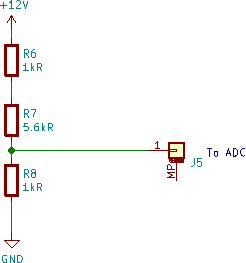
\includegraphics[width=.4\textwidth]{03voltage-div.pdf}
    \caption{The voltage divider circuit. J5 is supposed to connect to the analog input pin of the MCU.}
    \label{fig:03voltage-div}
\end{figure}

One can calculate the voltage ratio by:

\begin{equation}
    H_{ADC}=\frac{R8}{R6+R7+R8}=\frac{1}{7.6}
\end{equation}

\section{Battery System}

Piranha uses two paralleled connected Lithium-ion battery modules from BlueRobotics Inc. Each of them comprises 24 SAMSUNG INR18650-30Q cells, combined in a 4S6P configuration, shown in the Figure \ref{fig:03battery}. Table \ref{table:03battery} lists the technical specification of a single module.

\begin{figure}[ht]
    \centering
    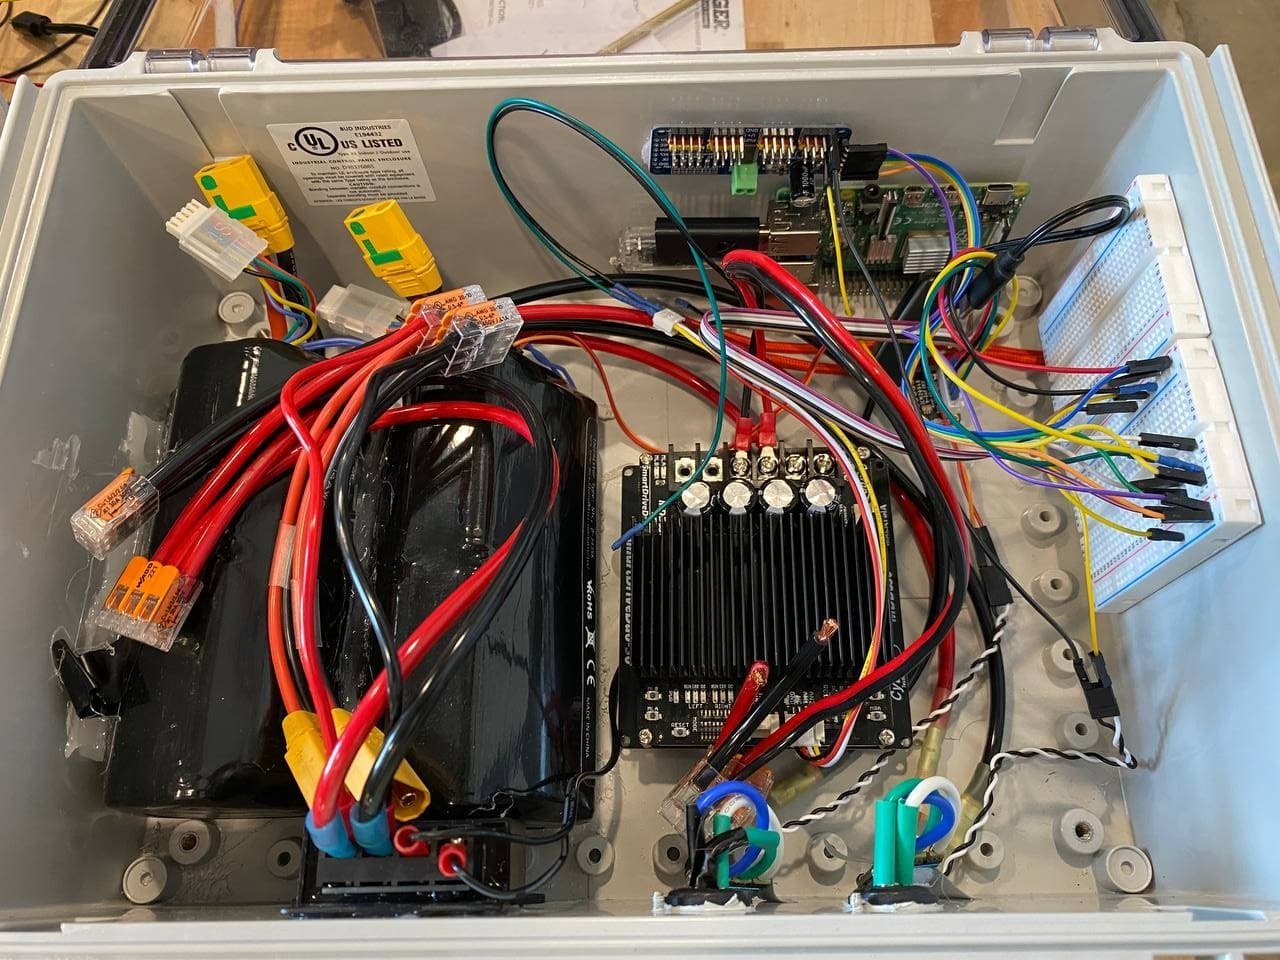
\includegraphics[width=.6\textwidth]{images/03batterysystem.jpg}
    \caption{I took the picture at an early stage test. The battery packs on the left are glued to the box to prevent collisions.}
    \label{fig:03battery}
\end{figure}

\begin{table}[ht]
\caption{Technical Specifications of BlueRobotics Lithium-ion Battery Module ($14.8\ V,\ 18\ Ah$)} % title of Table
\centering % used for centering table
\renewcommand{\arraystretch}{0.8}
\begin{tabular}{l l} % centered columns (4 columns)
\hline
\textbf{Characteristics} & \textbf{Rating} \\ 
%heading
\hline % inserts single horizontal line
Nominal Voltage  & $14.8\ V$ \\
Nominal Capacity & $18.0\ Ah$ \\
Cell Configuration & $4S6P$ \\
Maximum Continuous Current Draw & $90\ A$ \\
\hline %inserts single line
\end{tabular}
\label{table:03battery} % is used to refer this table in the text
\end{table}


\section{Motors (BLDC)}

Piranha equipped two BlueRobotics T200 Thrusters at the rear, shown in Figure \ref{fig:03thruster-test}. By the aerospace terminology convention, these thrusters are called motors in this article. They generate the main propulsion force for the vehicle.

\begin{figure}[ht]
    \centering
    \includegraphics[width=.6\textwidth]{03thruster-test.png}
    \caption{I calibrated two thrusters with a game controller. The right thruster is spinning. Meanwhile, the left one is not moving.}
    \label{fig:03thruster-test}
\end{figure}

Table \ref{table:03motor} lists the technical specifications of the motor.

\begin{table}[ht]
\caption{Technical Specifications of BlueRobotics T200 Thruster (part)} % title of Table
\centering % used for centering table
\renewcommand{\arraystretch}{0.8}
\begin{tabular}{l c l} % centered columns (4 columns)
\hline
\textbf{Characteristics} & \textbf{Rating} \\
%heading
\hline % inserts single horizontal line
Full Throttle FWD/REV Thrust \@ Nominal (16 V) & $5.25\ /\ 4.1\ kgf$ \\
Operating Voltage & $7-20\ V$ \\
Full Throttle Current \@ Nominal (16 V) & $24\ A$ \\
Full Throttle Power \@ Nominal (16 V) & $390\ W$ \\
\hline
\end{tabular}
\label{table:03motor} % is used to refer this table in the text
\end{table}

\section{Electric Speed Controller (ESC)}

The speed controller model is BlueRobotics Basic ESC, shown in Figure \ref{fig:03esc}. The ESCs on Piranha are controlled by two pulse-width modulated signals (PWM) generated by Pi Pico.

\begin{figure}
    \centering
    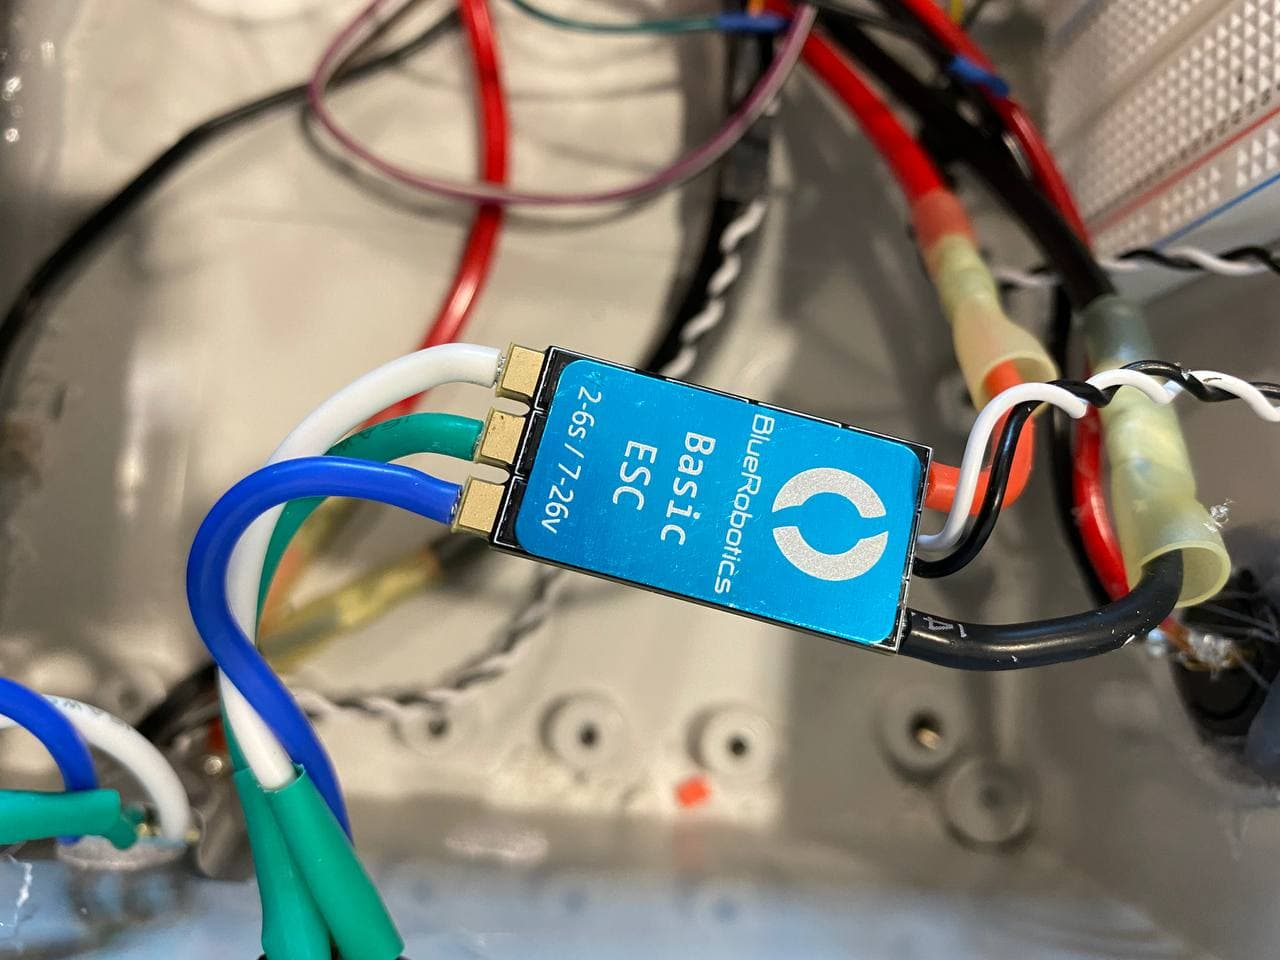
\includegraphics[width=.6\textwidth]{03esc.jpg}
    \caption{BlueRobotics Basic ESC.}
    \label{fig:03esc}
\end{figure}

Table \ref{table:03esc} lists their technical specifications.

\begin{table}[ht]
\caption{Technical Specifications of BlueRobotics Basic ESC (part)} % title of Table
\centering % used for centering table
\renewcommand{\arraystretch}{0.8}
\begin{tabular}{l c l} % centered columns (4 columns)
\hline
\textbf{Characteristics} & \textbf{Rating} \\ 
%heading
\hline % inserts single horizontal line
Operating Voltage & $7-26\ V$ \\
Maximum Current & $30\ A$ \\
Maximum Update Rate & $400\ {\rm Hz}$ \\
Stop Signal Width & $1500\ \mu s$ \\
Maximum Forward Signal Width & $1900\ \mu s$ \\
Maximum Backward Signal Width & $1100\ \mu s$ \\
\hline
\end{tabular}
\label{table:03esc} % is used to refer this table in the text
\end{table}

\section{MCU}

The microcontroller unit, also known as MCU, is the Pi Pico, designed and manufactured by Pi Foundation, shown in Figure \ref{fig:03pico}. Its specification can be found in Table \ref{table:03pico}.

\begin{figure}
    \centering
    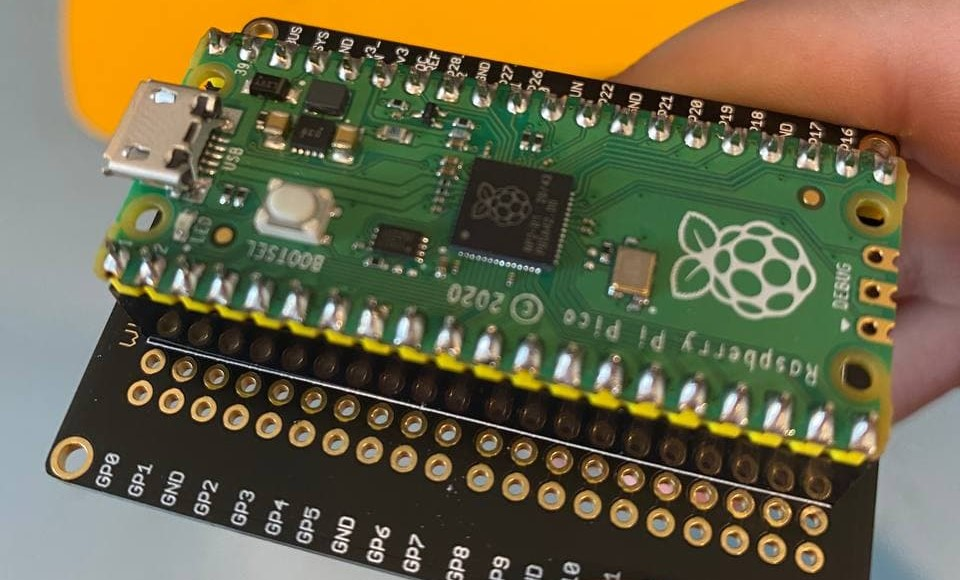
\includegraphics[width=.6\textwidth]{03pico.jpg}
    \caption{Pi Pico installed on the breakout board.}
    \label{fig:03pico}
\end{figure}

The chip model on the Pi Pico board is RP2040. It has a dual-core cortex M0+ at up to 133MHz frequency. For its specification, please refer to the extra document files.

\begin{table}[ht]
\caption{Electrical Specifications of Pi Pico (part)} % title of Table
\centering % used for centering table
\renewcommand{\arraystretch}{0.8}
\begin{tabular}{l c l} % centered columns (4 columns)
\hline
\textbf{Characteristics} & \textbf{Rating} \\ 
%heading
\hline % inserts single horizontal line
Supply Voltage & $1.8-5.5V$ \\
Operating Temperature & $-20 - 85\ \degree C$ \\
VBUS Current & $1.2-92.8\ mA$ \\
Flash Size & $2\ {\rm MByte}$ \\
\hline
\end{tabular}
\label{table:03pico} % is used to refer this table in the text
\end{table}

\section{IMU}

On Piranha, there are two IMUs. One is Adafruit TDK InvenSense ICM-20948 9-DoF shown as in Figure \ref{fig:03icm20948}, the other is Ceva BNO085 IMU, shown in Figure \ref{fig:03bno085}.  

ICM-20948 is the latest 9-axis MotionTracking device designed by TDK. It contains a 3-axis MEMS accelerometer, a 3-axis MEMS gyroscope, and a 3-axis MEMS magnetometer. It also has a built-in temperature sensor that can compensate for the error caused by the temperature shifting. The specification of ICM-20948 can be found in Table \ref{table:03icm20948}. ICM20948 features a built-in digital motion processor to process the acceleration data on the chip, so the Pi Pico can directly access the real-time position and speed data.

BNO085 is co-designed by Ceva and Bosch. Like ICM20948, it also integrates a triaxial accelerometer, a triaxial gyroscope, a magnetometer, and a 32-bit ARM® Cortex™-M0+ microcontroller running CEVA's SH-2 firmware that can output the integrated position result directly. Its specification can be found in Table \ref{table:03bno085}.

\begin{figure}[H]
    \centering
    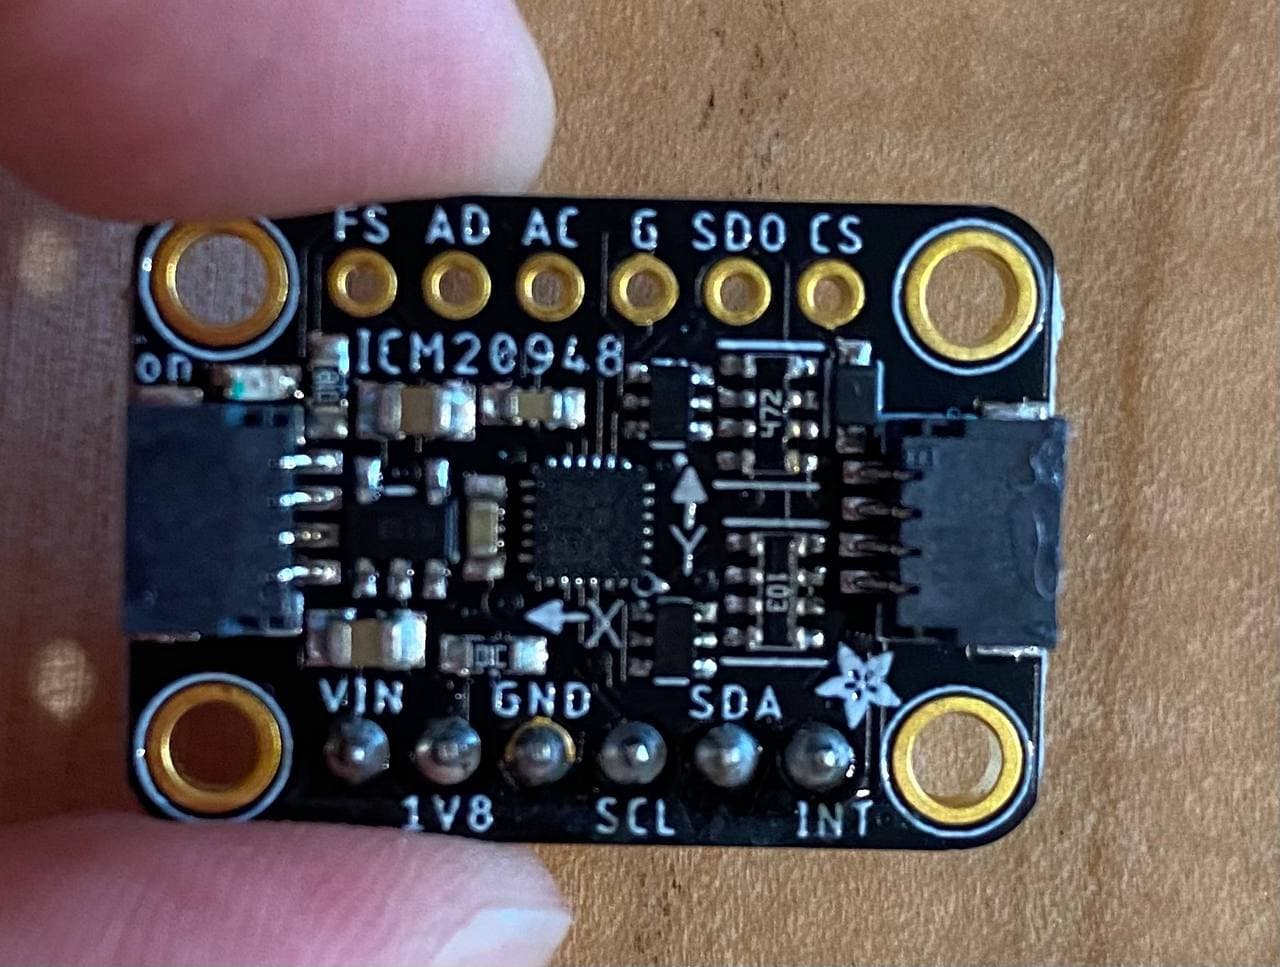
\includegraphics[width=.6\textwidth]{images/03icm20948.jpg}
    \caption{Adafruit TDK InvenSense ICM-20948 9-DoF IMU.}
    \label{fig:03icm20948}
\end{figure}

\begin{figure}[H]
    \centering
    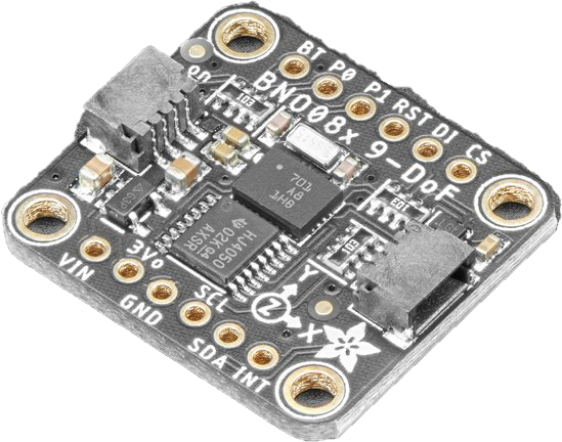
\includegraphics[width=.6\textwidth]{images/03bno085.png}
    \caption{Adafruit 9-DOF Orientation IMU Fusion Breakout - BNO085.}
    \label{fig:03bno085}
\end{figure}


\begin{table}[H]
\caption{Specification of ICM-20948 (part)} % title of Table
\centering % used for centering table
\renewcommand{\arraystretch}{0.8}
\begin{tabular}{l c l} % centered columns (4 columns)
\hline
\textbf{Characteristics} & \textbf{Rating} \\ 
%heading
\hline % inserts single horizontal line
Gyroscope Date Rate (Low Pass Filter On)& $1.125\ {\rm kHz}$ \\
Accelerometer Date Rate (Low Pass Filter On) & $1.125\ {\rm kHz}$ \\
Magnetometer Date Rate & $100\ {\rm Hz}$ \\
Gyroscope Full-Scale Range (GYRO\_FS\_SEL=0) & $\pm 250\ dps$ \\
Accelerometer Full-Scale Range (ACCEL\_FS=0) & $\pm 2\ G$ \\
Magnetometer Full-Scale Range & $\pm 4900\ \mu T$ \\

\hline
\end{tabular}
\label{table:03icm20948} % is used to refer this table in the text
\end{table}

\begin{table}[H]
\caption{Specification of BNO-085 (part)} % title of Table
\centering % used for centering table
\renewcommand{\arraystretch}{0.8}
\begin{tabular}{l c l} % centered columns (4 columns)
\hline
\textbf{Characteristics} & \textbf{Rating} \\ 
%heading
\hline % inserts single horizontal line
Gyroscope Date Rate (Low Pass Filter On)& $1\ {\rm kHz}$ \\
Accelerometer Date Rate (Low Pass Filter On) & $0.5\ {\rm kHz}$ \\
Magnetometer Date Rate & $100\ {\rm Hz}$ \\
Gyroscope Full-Scale Range (GYRO\_FS\_SEL=0) & $\pm 2000\ dps$ \\
Accelerometer Full-Scale Range (ACCEL\_FS=0) & $\pm 8\ G$ \\

\hline
\end{tabular}
\label{table:03bno085} % is used to refer this table in the text
\end{table}


\section{Magnetometer}

Since electromagnetic interference can easily disrupt magnetometer readings, Piranha also has a dedicated magnetometer, RM3100, installed away from the motors, batteries, and other electrical components. The RM3100 sensor is shown in Figure \ref{fig:03rm3100}, its technical specification is listed in Table \ref{table:03rm3100}.

\begin{figure}[ht]
    \centering
    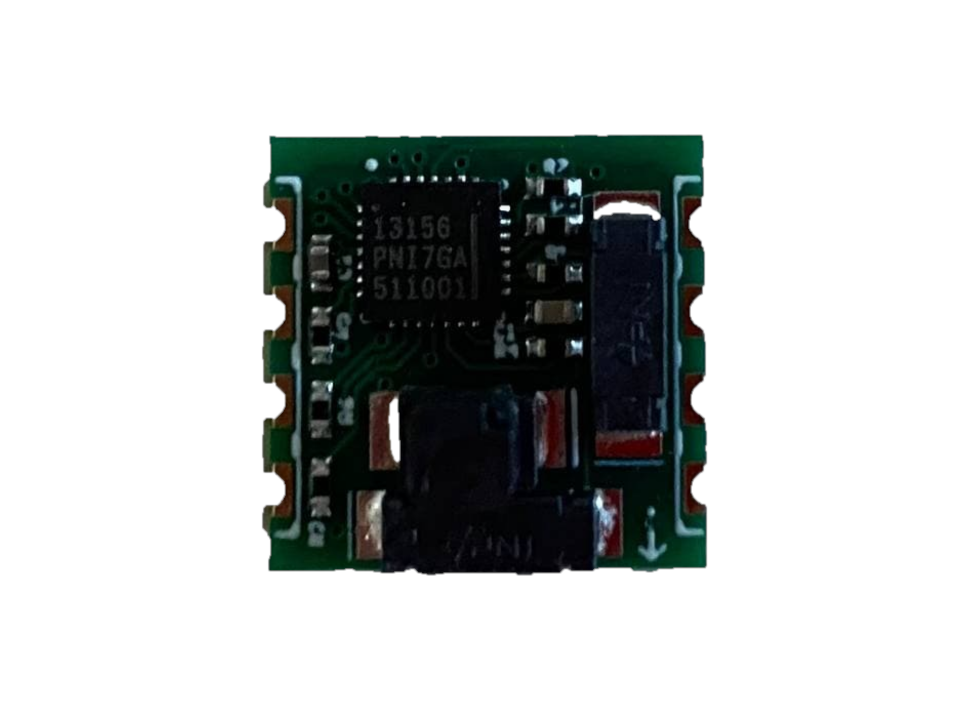
\includegraphics[width=.6\textwidth]{images/03rm3100.png}
    \caption{WitMotion High-Precision RM3100 Magnetometer Sensor}
    \label{fig:03rm3100}
\end{figure}

\begin{table}[ht]
\caption{Specifications of RM3100 (part)} % title of Table
\centering % used for centering table
\renewcommand{\arraystretch}{0.8}
\begin{tabular}{l c l} % centered columns (4 columns)
\hline
\textbf{Characteristics} & \textbf{Rating} \\ 
%heading
\hline % inserts single horizontal line
Maximum Single-Axis Sample Rate & 1600/850/440 Hz \\
DC Supply Voltage & $2.0\sim3.6$ V \\
Field Measurement Range & $-800 \sim 800\ m\mu$T \\
Sensitivity & 50/26/13 nT \\
Noise & 30/20/15 \\
\hline
\end{tabular}
\label{table:03rm3100} % is used to refer this table in the text
\end{table}

One must verify that sensitivity of the magnetometer measurement is high enough to detect the earth's magnetic field, which is approximately 0.6 Gauss (48A/m; 6000 nT), before using it. RM3100 has a measurement range within $\pm 800\ \mu$T or $\pm 8\times 10^5\ n$T, which is well more significant than the earth's magnetic field strength, and high sensitivity as low as $\pm 13\ n$T which is only $0.21\%$ of the earth's magnetic field strength. So it is reasonable to use RM3100 as a digital compass on Piranha.

In applications like small fixed-wing planes and rotors, the engineers often consider magnetometer readings very noisy because the electromagnetic interference is usually very high. However, on Piranha, because the magnetometer is put far from the interference source, we believe the data to be reliable and put more weight on them in the sensor fusion (EKF) part. This report will explain it later.

\section{GPS}

GPS is essential in the position estimation process because it provides drift-free position and speed data in real-time.

On Piranha, the GPS module is Adafruit Ultimate GPS, built around the MTK3339 chipset. Readers can find its technical specifications in Table \ref{table:03gps}.

\begin{table}[ht]
\caption{Specification of Adafruit Ultimate GPS (part)} % title of Table
\centering % used for centering table
\renewcommand{\arraystretch}{0.8}
\begin{tabular}{l c l} % centered columns (4 columns)
\hline
\textbf{Characteristics} & \textbf{Rating} \\ 
%heading
\hline % inserts single horizontal line
Satellites & 22 tracking, 66 searching \\
Update Rate & $1-10 {\rm Hz}$ \\
Position Accuracy & $<3 \ m$ \\
Velocity Accuracy & $<0.1\ m/s$ \\
Maximum Velocity & $515\ m/s$ \\

\hline
\end{tabular}
\label{table:03gps} % is used to refer this table in the text
\end{table}

\section{Wireless Module}

We designed Piranha with a manual mode, which allows the human operator to control the boat from a distance. During the development, we considered multiple different communication methods and tested them all. Table \ref{table:03wireless} shows the comparison among them.

\begin{table}[H]
\caption{Wireless Communication Method Comparison} % title of Table
\centering % used for centering table
\renewcommand{\arraystretch}{0.8}
\begin{tabular}{l l l l l} % centered columns (4 columns)
\hline
\textbf{Method} & \textbf{Speed} & \textbf{Range} & \textbf{Cost} & \textbf{Power Consumption} \\ 

%heading
\hline % inserts single horizontal line
4G/LTE & 100 Mbps & Depends on the coverage & High\footnotemark & $~100\ {\rm mW}$ \\
WiFi & 150 Mbps & $< 70\ {\rm ft}$ & Low & $~100\ {\rm mW}$ \\
RF Radio & 10 Mbps & $\sim 1\ {\rm mile}$ & High & $\sim 1\ {\rm W}$ \\
LoRa & $0.3- 20 {\rm kbps}$ & $\sim 5\ {\rm miles}$ & Low & $\sim 1\ {\rm W}$ \\
\hline
\end{tabular}
\label{table:03wireless} % is used to refer this table in the text
\end{table}

\footnotetext{Most 4G plans in the U.S. need a monthly payment.}

Piranha is a water surface robot, so its moving range depends on the control signal range if controlled by a human operator. For this reason, the control signal range should be as long as possible. Since the control signal only has simple commands, it does not need high bandwidth to work.

As a result, We chose to use LoRa on Piranha as the main wireless communication method from the ground station. LoRa is a wireless communication protocol based on the spread spectrum technology. It is designed for low power, and long-range data transmission \cite{8075570}. The LoRa module on Piranha is the Ebyte E32-915T30D model, shown in Figure \ref{fig:03e32}, it works on the $915 {\rm MHz}$ band. Because it works on an unlicensed band in the U.S., there is no need to get a commercial license from FCC. Its technical specification can be found in Table \ref{table:03e32}.

\begin{figure}
    \centering
    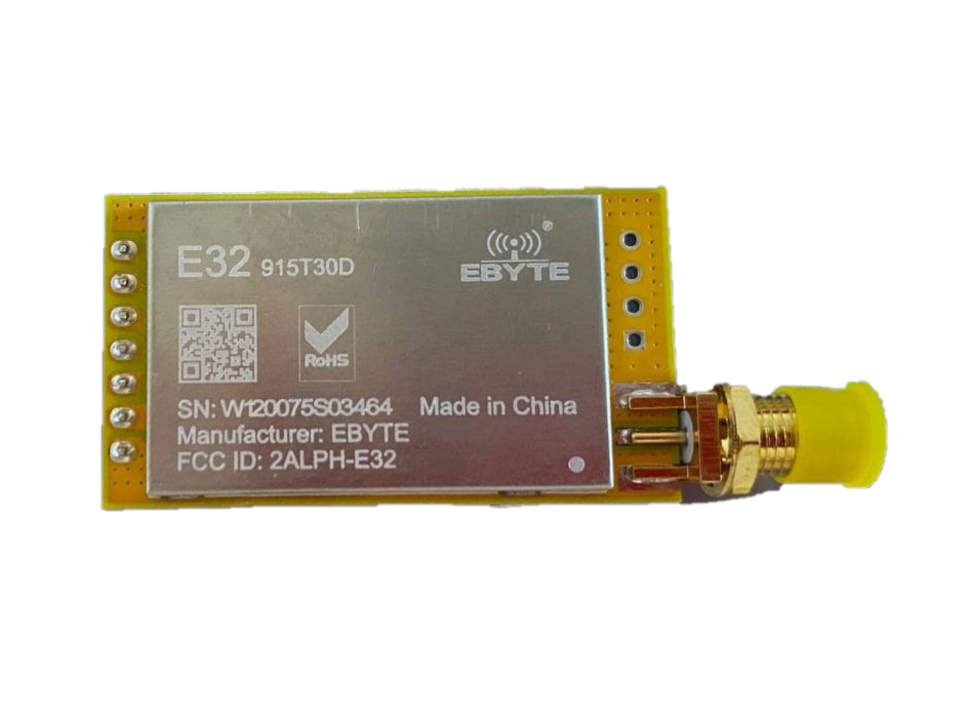
\includegraphics[width=.6\textwidth]{images/03e32.png}
    \caption{E32-915T30D}
    \label{fig:03e32}
\end{figure}

\begin{table}[H]
\caption{Specifications of E32-915T30D} % title of Table
\centering % used for centering table
\renewcommand{\arraystretch}{0.8}
\begin{tabular}{l l l l l} % centered columns (4 columns)
\hline
\textbf{Characteristics} & \textbf{Rating} \\ 
%heading
\hline % inserts single horizontal line
Maximum Transmission Power & $1\ {\rm W}$ \\
Maximum Communication Distance & $8\ {\rm km}$ \\
Air Date Rate & $0.3-19.2$ kbps \\
Maximum Tx Power & $30\ {\rm dBm}$ \\
Maximum Rx Power & $-147\ {\rm dBm}$ \\
\hline
\end{tabular}
\label{table:03e32} % is used to refer this table in the text
\end{table}

\chapter{Simulation}

Simulation is an essential step in the control system design. The simulation model should reflect the dynamics property of the controlled target as close as possible. With a simulated model, engineers can first design and test the controller in the virtual environment and then deploy them in the real world. 

The advantage of a simulation-based development is that it will not cause any damage to the original model, which is usually very expensive and hard to build. Second, engineers can obtain the results in the computer faster than in the real world, which means we can get the results of a simulated test way more quickly than a real field test.

This chapter is about the simulation of Piranha. The formulation is based on a 6-DoF non-linear rigid body system. Unlike ground vehicles like rovers and cars, a water surface vehicle like Piranha has much more complicated dynamics because of fluid mechanics.

The most common ways to formulate the EOM of a given system are either through Lagrangian mechanics or Newtonian mechanics. Because the simulation only has one rigid body target, we preferred Newton's Law in this application. However, Newton's Law only holds within the inertial frame. Here, some assumptions are made before the EOM formulation to ensure this condition is met \cite{nahon1996simplified}.

\section{Assumptions}

Before the formulation, we made a few assumptions to rule out some unnecessary factors to consider, such as the Coriolis force and the earth's curvature. The assumptions include:

\begin{enumerate}
    \item The water surface is calm and flat without any curves.
    \item The vehicle is a rigid body with a constant mass. 
    \item The gravitational acceleration is also a constant value.
    \item The simulated world does not rotate.
    \item The fluid has a constant current direction and speed, as well as the wind.
\end{enumerate}

These assumptions make sure that the simulation world frame is inertial. In other words, we can use Newton's Second Law to formulate the equations of motion.

\section{6 DoF State-Space Equations of Motion}

The equation of motion has 6 degrees of freedom. To simplify the formulation, the state vector $\boldsymbol{X}$ is divided into two parts, $\boldsymbol{x}$ and $\boldsymbol{\nu}$.

\begin{equation}
    \boldsymbol{X}=\left[\begin{aligned}
        &\ \boldsymbol{x}\ \\
        &\ \boldsymbol{\nu}\
    \end{aligned}\right]
\end{equation}

We define $\boldsymbol{x}$ as the position vector, $\boldsymbol{\nu}$ as the velocity vector. They are attached to different reference frames, $\boldsymbol{x}$ is attached to the ground NED frame while $\boldsymbol{\nu}$ is linked to Piranha's body frame.

\begin{align}
    \boldsymbol{x} & =[p_n, p_e, p_d, \phi, \theta, \psi]^\top \\
    \boldsymbol{v} & =[u, v, w, p, q, r]^\top
\end{align}

The input vector of the system $\boldsymbol{u}_{\rm PWM}$ consists of the PWM input values for the left and right thrusters. 

We can write the EOM of this system as:

\begin{equation}
    \boldsymbol{M\dot{\nu}}+\boldsymbol{C}(\boldsymbol{x},\boldsymbol{\nu},\boldsymbol{w}_c)+\boldsymbol{D}(\boldsymbol{x}, \boldsymbol{\nu}, \boldsymbol{w}_a)+\boldsymbol{G}=\boldsymbol{\tau}
\end{equation}

$\boldsymbol{M}$ is the mass matrix, $\boldsymbol{C}(\boldsymbol{x},\boldsymbol{\nu},\boldsymbol{w}_c)$ is the fluid dynamical matrix, $\boldsymbol{w}_c$ is the water current vector, $\boldsymbol{D}(\boldsymbol{x}, \boldsymbol{\nu}, \boldsymbol{w}_a)$ is the air dynamical matrix, $\boldsymbol{w}_a$ is the wind speed vector, $\boldsymbol{G}$ is the gravity matrix, $\boldsymbol{\tau}(\boldsymbol{u}_{\rm PWM})$ is the mapped input vector of the system, the transformation will be discussed in after a few sections.

\section{Reference Frames}

In the state-space representation shown above, we represent all components as vectors. However, these vectors in the simulation EOM link to different frames, such as the input vector $\boldsymbol{\tau}(\boldsymbol{u}_{\rm PWM})$ is in the body frame. Meanwhile, the gravitational component $G$ is a constant vector in the ground frame.

To begin with, here list five types of frames in the simulation:

\begin{itemize}
    \item Earth-Centered Inertial (ECI) frame.
    \item Earth-Centered, Earth-Fixed (ECFF) frame.
    \item Ground North, East, Down (NED) frame.
    \item Local North, East, Down frame.
    \item The Body frame.
\end{itemize}

Because the assumptions rule out the world's rotation, the Coriolis effect does not exist in the simulation. Because Piranha only moves on the surface of the earth, we consider the $\boldsymbol{x}$ position vector is in the ground NED frame rather than the ECFF frame and ECI frame.

Since we use Newton's Law for building the simulation EOM, every component inside the equation is relative to the body frame. However, some parts like the wind speed vector and the gravity matrix are initially constant in the local NED frame, so we must transform them into the same frame first.

\subsection{Transform Vectors from Local NED Frame to Body Frame}

With the roll, pitch, yaw angles to be $[\phi, \theta, \psi]$, the transform matrix can be described by:

\begin{equation}
    R_1=\left[\begin{array}{rrr}
        \cos(\psi) & \sin(\psi) & 0  \\
        -\sin(\psi) & \cos(\psi) & 0 \\
        0 & 0 & 1 
    \end{array}\right]
\end{equation}

\begin{equation}
    R_2=\left[\begin{array}{rrr}
        \cos(\theta) & 0 & -\sin(\theta)  \\
        0 & 1 & 0 \\
        \sin(\theta) & 0 & \cos(\theta) 
    \end{array}\right]
\end{equation}

\begin{equation}
    R_3=\left[\begin{array}{rrr}
        1 & 0 & 0  \\
        0 & \cos(\phi) & \sin(\phi) \\
        0 & \sin(\phi) & \cos(\phi) 
    \end{array}\right]
\end{equation}

\begin{equation}
    \boldsymbol{x}_{\rm body}=R_3R_2R_1\boldsymbol{x}_{\rm ground}
\end{equation}

\section{Mass Matrix}

First decompose the velocity vector $\boldsymbol{\nu}$ into linear movement $\boldsymbol{\nu}_l=[u,\ v,\ w]$ and rotation parts $\boldsymbol{\nu}_r=[p,\ q,\ r]$. The mass matrix can also be split into the linear mass matrix $\mathbf{M}_l$ and the inertia matrix $\mathbf{M}_r$.

\begin{equation}
    \mathbf{M}=\left[\begin{array}{cc}
        \mathbf{M}_l & \boldsymbol{0} \\
        \boldsymbol{0} & \mathbf{M}_r
    \end{array}\right]
\end{equation}

Where,

\begin{equation}
    \mathbf{M}_l = m\mathbf{I}\quad \mathbf{M}_r=\left[\begin{array}{ccc}
        I_{xx} & I_{xy} & I_{xz} \\
        I_{yx} & I_{yy} & I_{yz} \\
        I_{zx} & I_{zy} & I_{zz} \\
    \end{array}\right]
\end{equation}

And,

\begin{align}
    \mathbf{F} &=\mathbf{F}_0+\Delta\mathbf{F} \\
    \mathbf{T} &=\mathbf{T}_0+\Delta\mathbf{T}
\end{align}

$\mathbf{F}_0$ and $\mathbf{T}$ is the theoretical force and torque. The $\Delta$ denotes the perturbation in the real-world model. In this section, we ignore this perturbation.

With Newton's Law,

\begin{equation}
    \mathbf{F}=\left[\begin{array}{ccc}
        m\dot{u} & \cdots & 0 \\
        \vdots & m\dot{v} & \vdots\\
        0 & \cdots & m\dot{w}
    \end{array}\right]\quad \mathbf{T}=\left[\begin{array}{ccc}
        I_{xx} & I_{xy} & I_{xz} \\
        I_{yx} & I_{yy} & I_{yz} \\
        I_{zx} & I_{zy} & I_{zz}
    \end{array}\right]\left[\begin{array}{c}
        \dot{p} \\
        \dot{q} \\
        \dot{r}
    \end{array}\right]
\end{equation}

\begin{equation}
    \mathbf{M}\dot{\mathbf{\nu}}=\left[\begin{array}{cc}
        \mathbf{F} & \boldsymbol{0}  \\
        \boldsymbol{0} & \mathbf{T}
    \end{array}\right]
\end{equation}

In the simulation, these values are obtained from SOLIDWORKS Mass Properties, shown in Figure \ref{fig:04mass}:

\begin{figure}[ht]
    \centering
    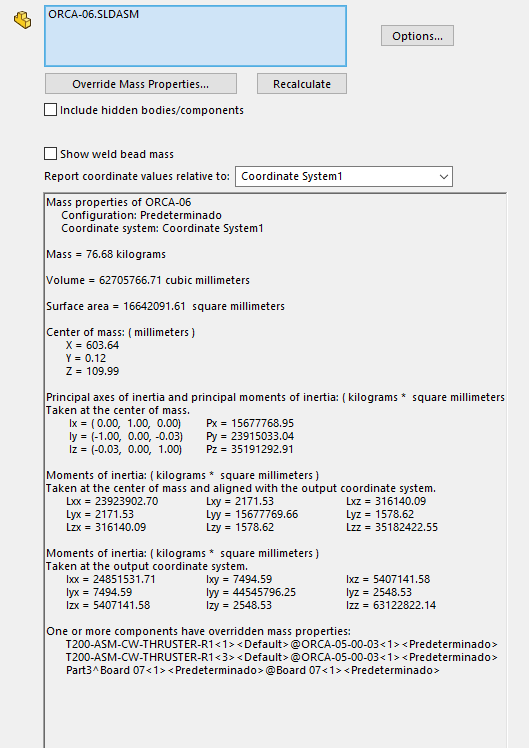
\includegraphics[width=.5\textwidth]{images/04solidworks.png}
    \caption{The mass matrix values of Piranha generated in the SOLIDWORKS Mass Properties menu.}
    \label{fig:04mass}
\end{figure}

\section{Fluid Dynamical Model}

The fluid dynamical model includes two parts, hydrostatic and hydrodynamic parts.

\subsection{Hydrostatic analysis}

In the hydrostatic part, the goal of the simulator is to estimate the whole buoyant force applied to Piranha and the buoyancy center, given the position of the boat. In Figure \ref{fig:04smodel}, we can see that the buoyancy estimation includes the center of buoyancy estimation and the upward force estimation. According to Archimedes' principle, we can calculate the upward buoyant force through the volume of the displaced water. 


\begin{figure}
    \centering
    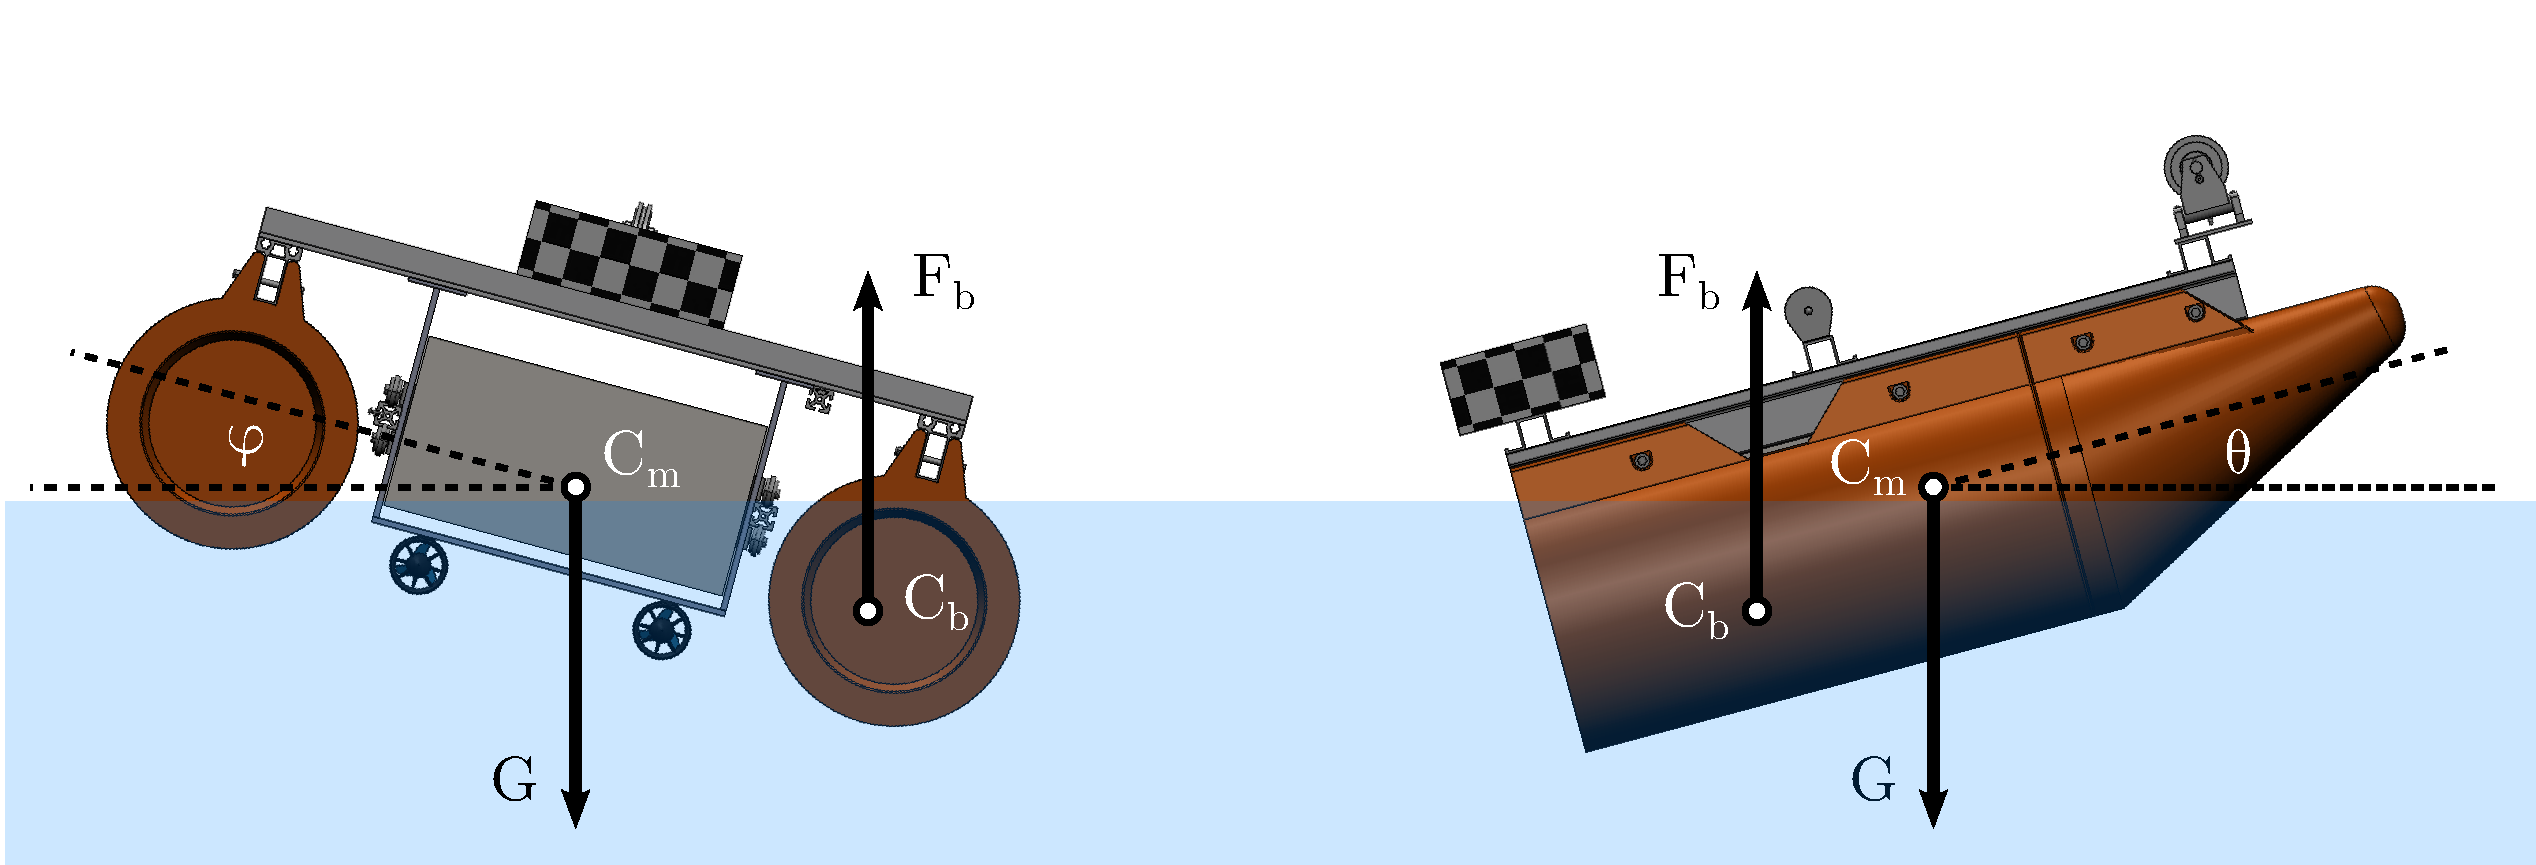
\includegraphics[width=.8\textwidth]{images/04hydrostatic.pdf}
    \caption{Hydrostatic model of Piranha.}
    \label{fig:04smodel}
\end{figure}

We can get estimations with pure mathematical calculation. For simplicity, here we do the math in the body frame. The first step is to transform the water level back to the Piranha's body frame, shown in the following equation.

\begin{equation}
    F_{wg}(x,y)=0 \longrightarrow F_{wb},\quad F_{wg}, \ F_{wb} \in R^2 
\end{equation}

We can consider the water level surface as a plane under the assumptions. So the equation of a plane in 3D space is:

\begin{equation}
    ax+by+cz=d
\end{equation}

The normal vector can be represented as $\boldsymbol{n_1}=[a, b, c]^\top$. We can determine the water surface in the body frame by solving this equation:

\begin{equation}
        R_v^b\boldsymbol{n_1} \cdot \boldsymbol{x}^\top_{(x=0,y=0)} = p_d
\end{equation}

There are three cases in calculating integral:

\begin{enumerate}
    \item The water level surface only intersects the lower half part of the float.
    \item The water level surface only intersects the upper half part of the float.
    \item The water level surface intersects both the upper and lower halves of the float.
\end{enumerate}

For all three cases, the integral can be represented as the following equation, denote $F_s$ to be the separate plane:

\begin{equation}
    V=\iint_{A_{xy}} \left[\min(\max(F_w-F_s,0),F_u-F_s) + \min(\max(F_w-F_l,0),F_s-F_l)\right]
\end{equation}

Because it is not a differentiable function due to $min$ and $max$ operators, but it can be solved using modern numerical methods. The formulation is not exclusive. These variables inside the integrated function can be $(x,z)$ instead of $(x,y)$. However, the function is always not differentiable. 

The buoyancy center is the mass center of the displaced water, thus can be calculated by the center of mass formula:

\begin{align}
    & M_{yz} =\iiint x\rho(x,y,z)\ {\rm d}V \\
    & M_{xz} =\iiint y\rho(x,y,z)\ {\rm d}V \\
    & M_{xy} =\iiint z\rho(x,y,z)\ {\rm d}V \\
    & \overline{x} =\frac{M_{yz}}{m},\ \overline{y} =\frac{M_{xz}}{m},\ \overline{z} =\frac{M_{xy}}{m}
\end{align}

\subsection{Hydrodynamic analysis}

The hydrodynamic analysis calculates the parasitic forces in the simulation. This process in real-life applications is usually handled by using modern CFD simulators to solve the Navier-Stokes equations. 

Although the CFD simulation precision depends on the fineness of the mesh, limited by today's computer technology, the CFD simulation is not real-time. Usually, it takes a long time, ranging from a few minutes to hours, to calculate for a set of given parameters. However, the CFD simulation needs to run from tens to thousands of times per second in the simulation scenarios, depending on the time step. As a result, the time cost for calculating hydrodynamics using common CFD software is unacceptable in the simulation.

The following section introduces an algorithm, which is used in Piranha's simulation code. This algorithm takes a triangle mesh as the input model and does the hydrostatic and hydrodynamic estimation at the cell level first. After that, it sums up all results and produces a general estimate of the buoyancy and drag on the whole body of the boat.

\section{Numerical Calculation}

This section covers the numerical methods used in Piranha's simulation program. We cannot calculate the theoretical equation efficiently in the computer. As a result, a simplified mesh model of Piranha is used to accelerate the calculation.

\subsection{Mesh Simplification}

The first step is to simplify the mesh and reduce the number of triangles to reduce the calculation time cost. The aim is to use the fewest triangles but maintain the shape of the original model.

We represent Piranha's simulation model with two cylinders and two cones, shown in Figure \ref{fig:04mesh}. 

\begin{figure}[H]
     \centering
     \hspace{1cm}
     \begin{subfigure}[b]{0.4\textwidth}
         \centering
         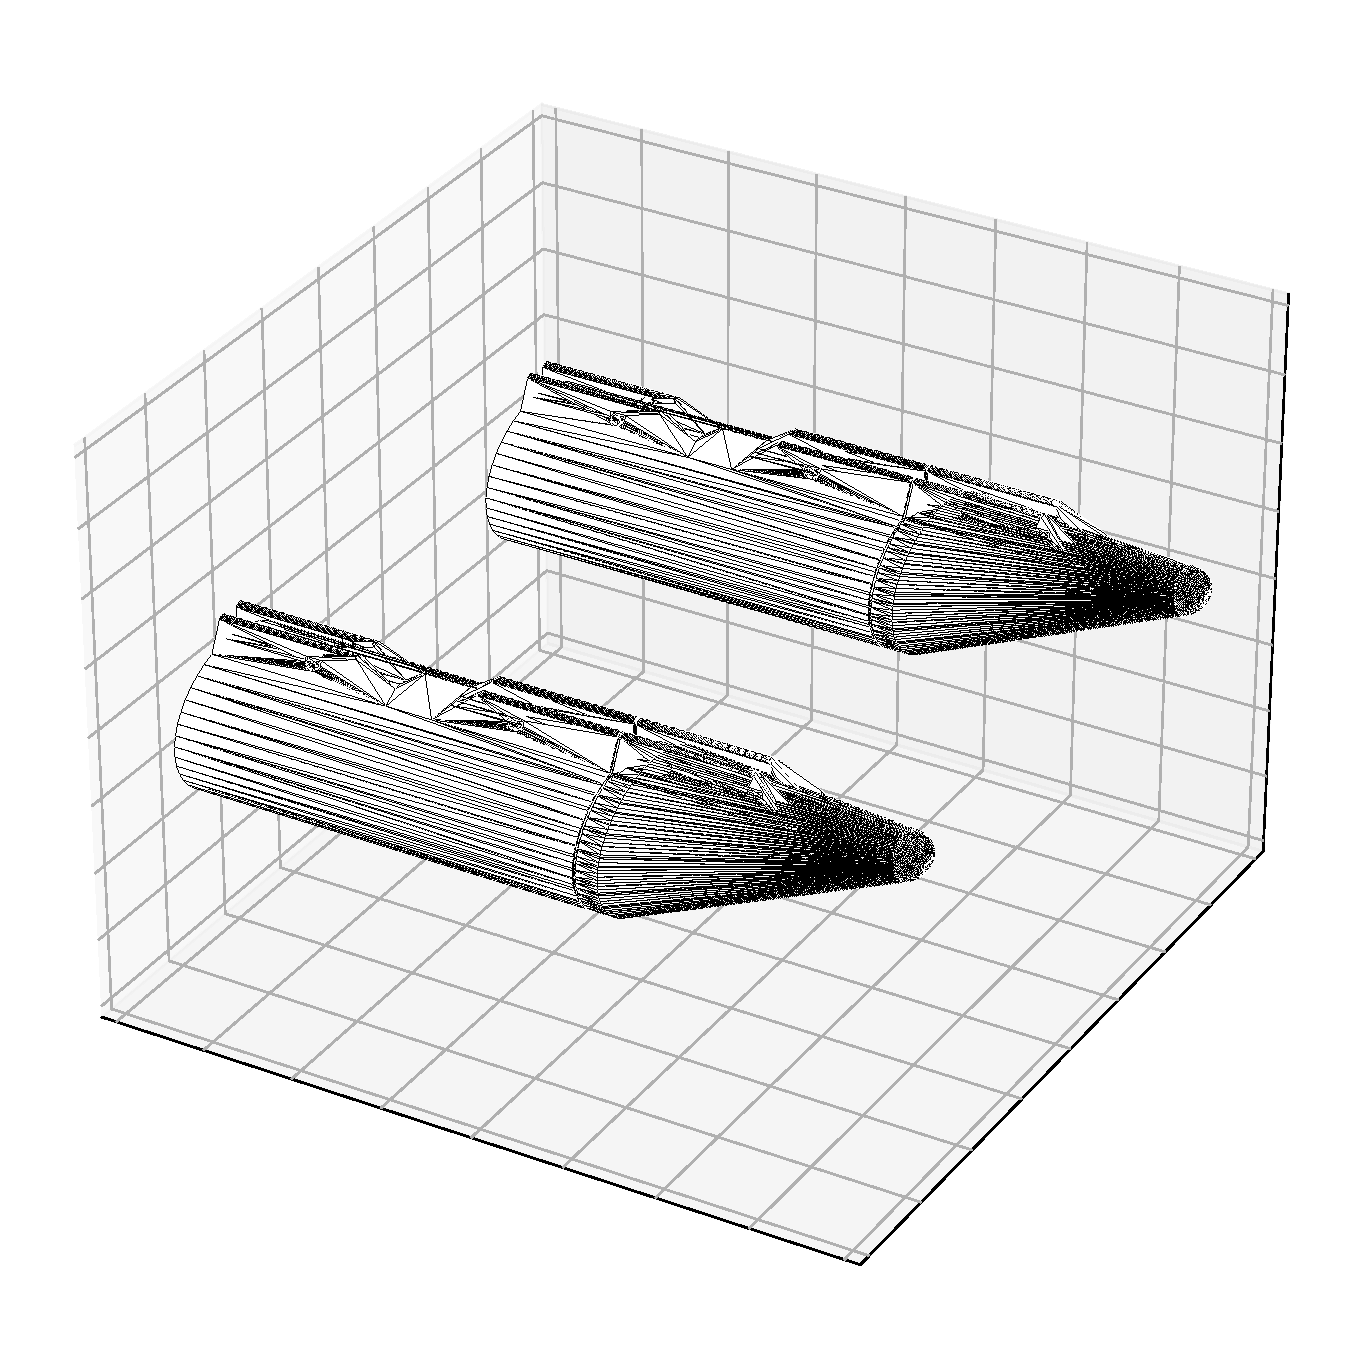
\includegraphics[width=\textwidth]{images/04orca_pontoon.pdf}
     \end{subfigure}
     \hfill
     \begin{subfigure}[b]{0.4\textwidth}
         \centering
         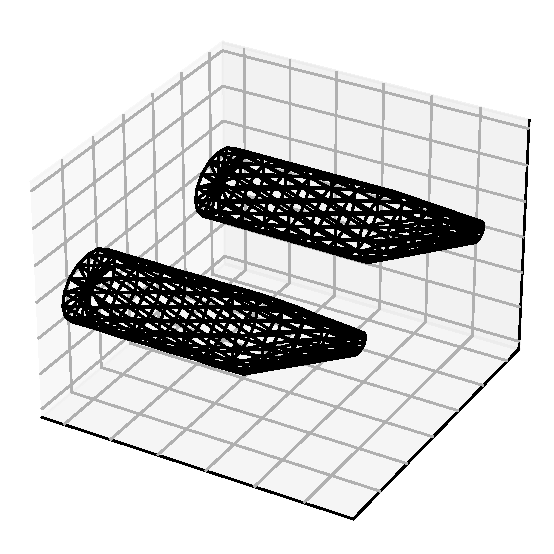
\includegraphics[width=\textwidth]{images/04mesh_orca.pdf}
     \end{subfigure}
     \caption{On the left is the original mesh generated by SOLIDWORKS, on the right is the simplified mesh model.}
     \label{fig:04mesh}
     \hspace{1cm}
\end{figure}

\subsubsection{Buoyancy Estimate}

The key to estimating buoyancy is to calculate the submerged volume. For a single triangle in the mesh, we can calculate its volume by the surface integral over the projected area, shown in the following equations.

\begin{equation}
    \boldsymbol{V} = \int_S F(x,y)\ {\rm d}x{\rm d}y
\end{equation}
   
\begin{equation}
    F(x,y)= \left\{\begin{aligned}
        f(x,y) &, f(x,y)>0 \\
        0 &, f(x,y)\leq 0
    \end{aligned}\right.
\end{equation} 

Given the triangle plane function $z=f(x,y)$.

If we ignore every triangle that is not fully submerged, there is also another way to calculate the volume under a triangle without using integration.

If we have a 3D triangle defined by $(x_1,y_1,z_1)$, $(x_2,y_2,z_2)$, $(x_3,y_3,z_3)$. Assume they are arranged in the order that $z_1<z_2<z_3$.

Assume there is a horizontal plane $P$, in other words, a plane that is parallel to $XY$ plane crossing the middle point $(x_2,y_2,z_3)$, $P$ divides the 3D triangle into upper and lower parts like Figure \ref{fig:04triangle-volume}.

\begin{figure}[ht]
    \centering
    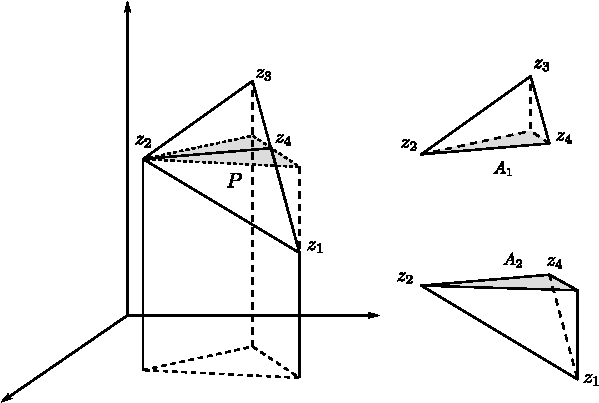
\includegraphics[width=.8\textwidth]{images/04triangle-volume.pdf}
    \caption{$A_1$ and $A_2$ are the projected area of the upper part and the lower part on the plane $P$.}
    \label{fig:04triangle-volume}
\end{figure}

We can calculate the volume of the 3D triangle given above as the volume of the triangular prism made by $P$, plus the upper triangular cone, minus the lower triangular cone, equals to:

\begin{equation}
    V=(A_1+A_2)z_2+\frac{1}{3}A_1(z_3-z_2)-\frac{1}{3}A_2(z_2-z_1)
\end{equation}

The projected area $A_1$ and $A_2$ can be calculated by:

\begin{align}
    A_1  & =  \frac{1}{2}[(x_4y_2-x_2y_4)+(x_3y_4-x_4y_3)+(x_2y_3-x_3y_2)] \\
    A_2  & =  \frac{1}{2}[(x_1y_2-x_2y_1)+(x_4y_1-x_1y_4)+(x_2y_4-x_4y_2)]
\end{align}

Where $(x_4,y_4,z_4)$ is the intersection point between $(x_3,y_3,z_3)$ and $(x_1,y_1,z_1)$. Apparently because $(x_4, y_4, z_4)$ is on $P$, $z_4=z_2$. $x_4$ and $y_4$ are given by:

\begin{align}
    x_4 &= x_1 + ((z_2-z_1)/(z_3-z_1)) (x_3-x_1) \\
    y_4 &= y_1 + ((z_2-z_1)/(z_3-z_1)) (y_3-y_1)
\end{align}

Substitute back and simplify the equation. In the end, the volume under a 3D triangle can be calculated by:

\begin{equation}
    V_{tri}  =  \frac{1}{6}(z_1+z_2+z_3)(A_1+A_2)=\frac{1}{6}(z_1+z_2+z_3)A_{proj}
\end{equation}

The volume equation can be interpreted as the "average height" times the projected area times $1/2$.

We can calculate the projected area through the cross product:

\begin{equation}
    A_{proj}=\frac{1}{2}|\boldsymbol{u}\times\boldsymbol{v}|
\end{equation}

There is no need for the computational heavy integration step when calculating the volume with this volume formula. However, we can only use it when the triangle is fully submerged.

However, if a triangle is not fully submerged, it is either partially submerged or not submerged at all. For the latter case, we can ignore the triangle. For the partially submerged case, there are two chances:

\begin{enumerate}
    \item Only one vertex is in the water.
    \item Two vertices are in the water.
\end{enumerate}

The simulator takes extra steps for these two cases, shown in Figure \ref{fig:04two-cases}. The key is to find the two intersection points and calculate the cone volume.


\begin{align}
    \text{For case 1:} & \quad V=V_{cone} \\
    \text{For case 2:} & \quad V=V_{tri}+V_{cone}
\end{align}

\begin{figure}[ht]
    \centering
    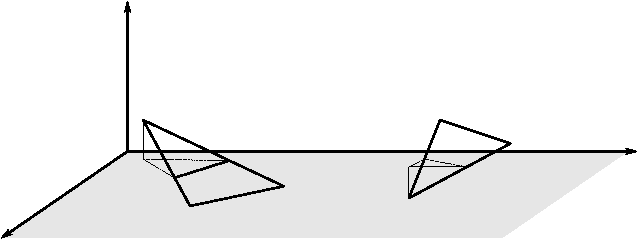
\includegraphics[width=.8\textwidth]{images/04two-cases.pdf}
    \caption{Two partially submerged cases.}
    \label{fig:04two-cases}
\end{figure}

Given the volume formula, it is easy to calculate the underwater volume for one triangular cell. The next step is to repeat this step for each triangle and sum up the results.

The face direction determines the volume should be taken from the sum, or added to the result, shown in Figure \ref{fig:04face-direction}. 

\begin{figure}[ht]
    \centering
    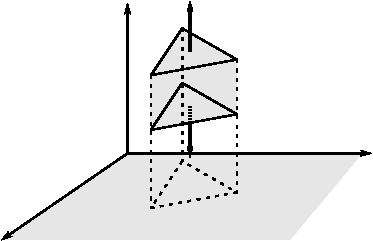
\includegraphics[width=.6\textwidth]{images/04face-direction.pdf}
    \caption{The offset water volume is between the two triangles. The face directions for the two triangles are different.}
    \label{fig:04face-direction}
\end{figure}

During the calculation, the program determines the face direction by the normal vector of the triangle. Due to this fact, the simulator saves the normal vectors and the triangle mesh for further calculation. These normal vectors, if visualized, can be seen in Figure \ref{fig:04normal-vector}:

\begin{figure}[H]
    \centering
    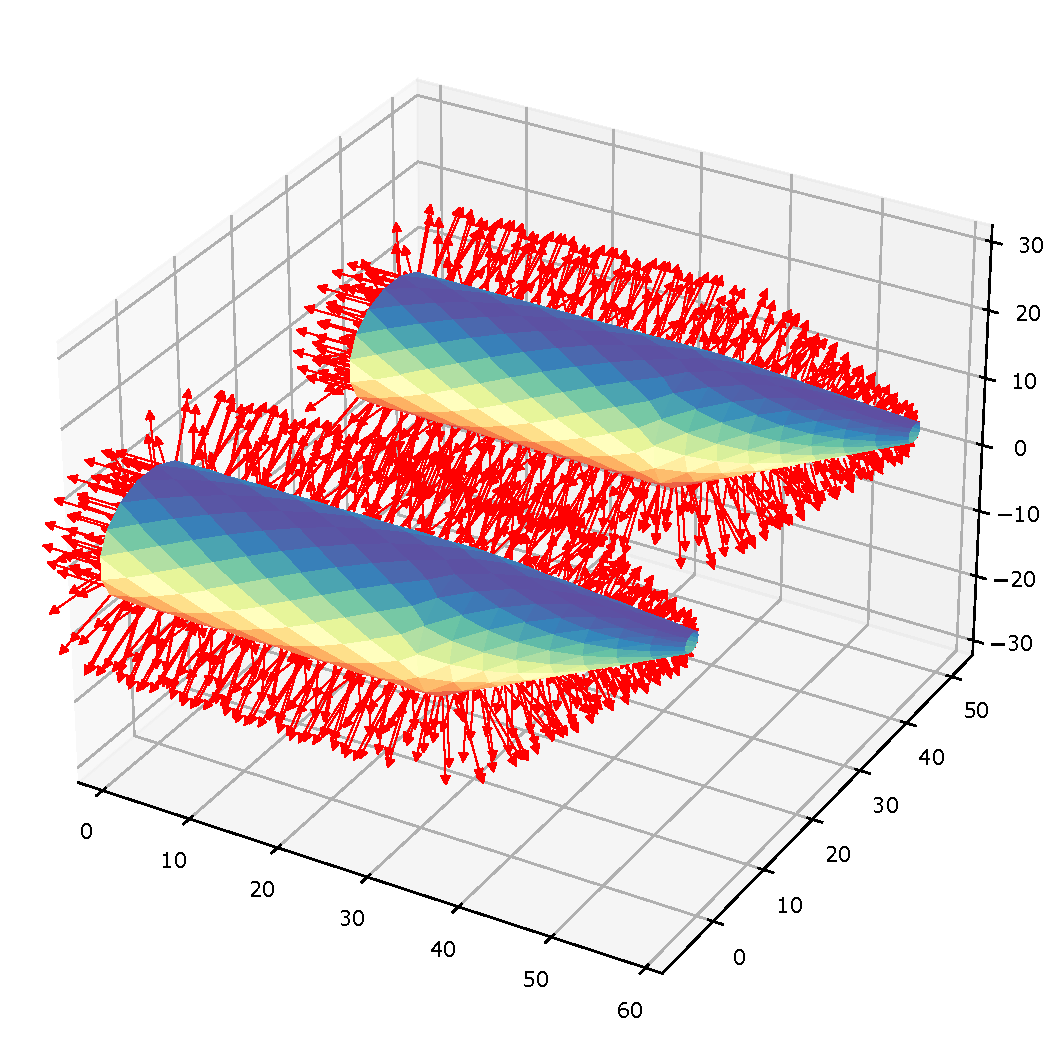
\includegraphics[width=.6\textwidth]{images/04normal-vector.pdf}
    \caption{In the mesh model, the area of a triangular face equals the length of its normal vector.}
    \label{fig:04normal-vector}
\end{figure}

Figure \ref{fig:04hydrostatic-flowchart} briefly illustrates the flowchart of the buoyancy estimate algorithm. However, in practice, the simulator does not follow this chart strictly. In the real world, the simulator combines the hydrostatic estimator and hydrodynamic estimator so that the face classification process only needs to run once for each face. The classification result is shared between both estimators for performance optimization.  

\begin{figure}[H]
    \centering
    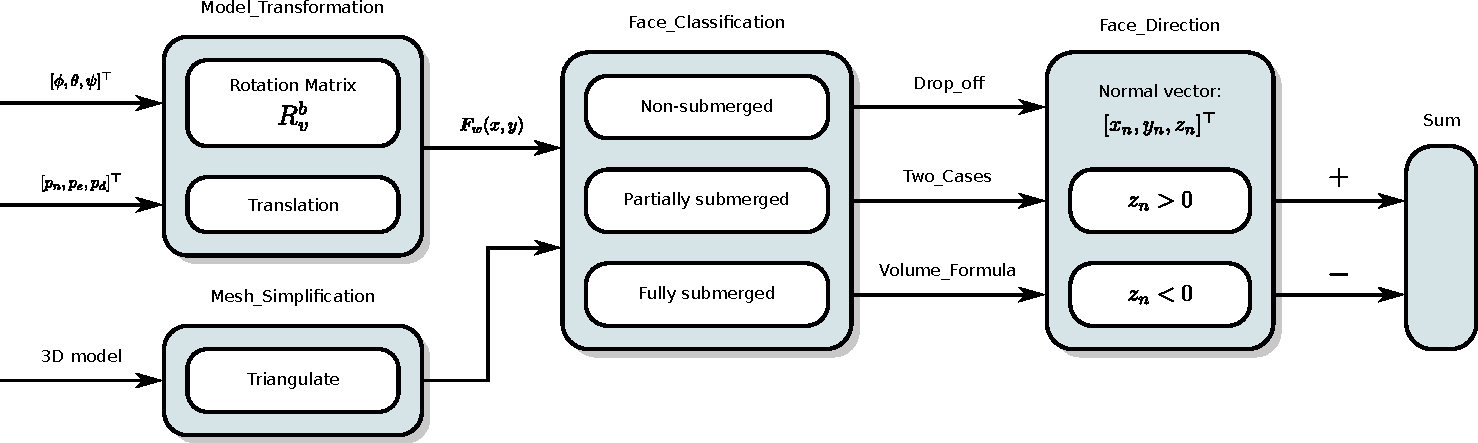
\includegraphics[width=\textwidth]{images/04hydrostatics_flowchart.pdf}
    \caption{Piranha's hydrostatic estimator flowchart.}
    \label{fig:04hydrostatic-flowchart}
\end{figure}

\subsubsection{Drag \& Skin Friction Estimate}

For simplicity, we only consider drag and skin friction in the simulation's hydrodynamics. The other factor like water waves and twirls are not considered here \cite{tian2015dynamic}. We can calculate these two forces through:

\begin{equation}
\begin{split}
    F_d &= \int C_{i0}+ C_{i1} \rho v_1 + C_{i2} \rho v_1^2  {\rm d} A \\
    F_f &= \int C_{f0}+ C_{f1} \rho v_2 C_{f2} \rho v_2^2 {\rm d} A
\end{split}
\end{equation}

However, unlike most common simulators, which only use a rough frontal area value in the formula, Piranha's simulator uses a more precise algorithm to calculate the frontal area.

The drag and skin friction are calculated independently for each triangular cell. The simulator sums up all the result values and synthesizes a general force and general torque to represent the hydrodynamic component, shown in Figure \ref{fig:04orca_surf}.

\begin{figure}
    \centering
    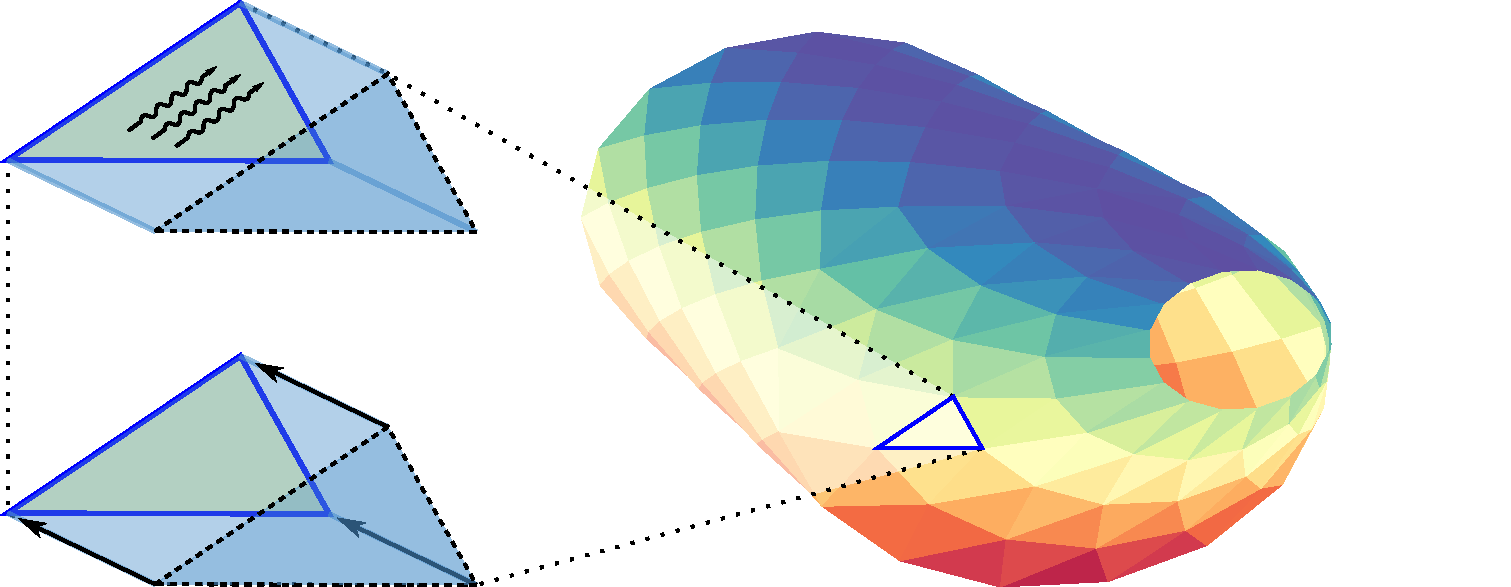
\includegraphics[width=.8\textwidth]{images/04orca_surf.pdf}
    \caption{Cell level dynamics, drag and skin friction.}
    \label{fig:04orca_surf}
\end{figure}

The hydrodynamics estimator flowchart can be found in Figure \ref{fig:04hydrodynamic-flowchart}.

\begin{figure}
    \centering
    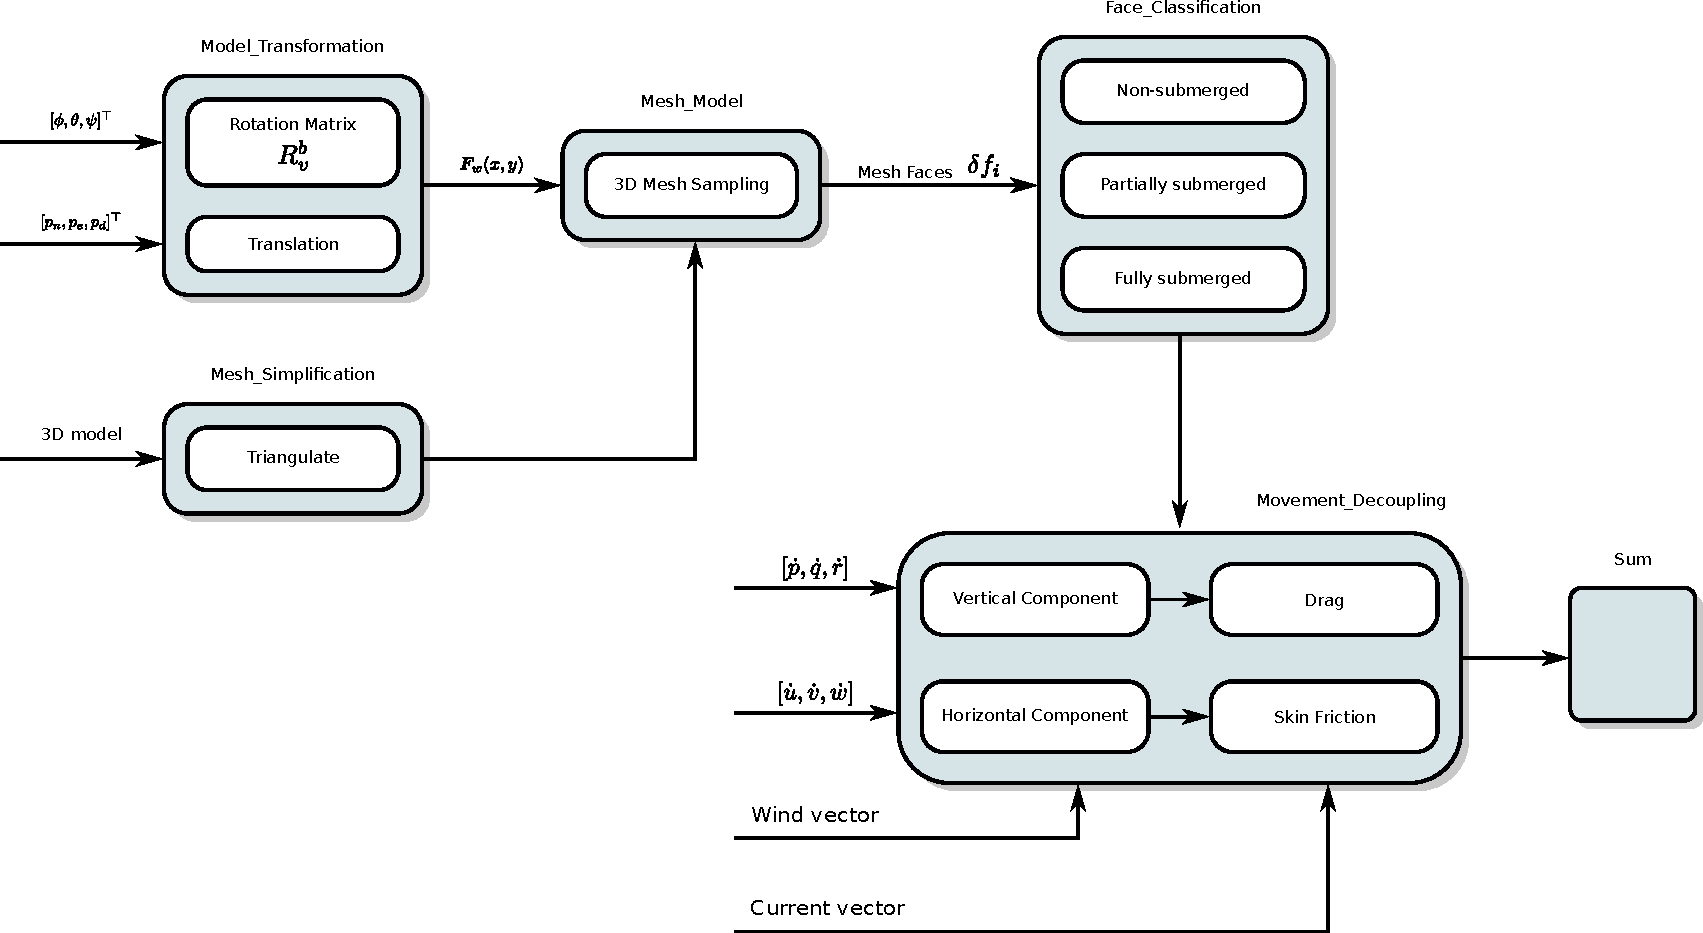
\includegraphics[width=\textwidth]{images/04hydrodynamics_flowchart.pdf}
    \caption{Piranha's hydrodynamic estimator flowchart.}
    \label{fig:04hydrodynamic-flowchart}
\end{figure}

The flowchart shows that each face is classified into different types according to the above discussion first. And for simplicity, the simulator ignores the skin friction component for the area in the air.

\subsubsection{Wind and Current Vectors}

Wind and water current have a significant effect on the simulation. Thus, the simulator cannot ignore them blindly. However, compared with hydrodynamics, the aerodynamics of Piranha is of less importance.

In the simulation, these factors are considered in the hydrodynamics estimation part, as shown in Figure \ref{fig:04hydrodynamic-flowchart}. While calculating the drag and friction for a face, the simulator first calculates a relative speed for the wind frame and water current frame, then proceeds to the movement decoupling step and applies drag and skin friction coefficients correspondingly.

\section{Input Mapping}

The simulation input is the PWM control signal widths of the two thrusters, which are controllable by the embedded controller. However, the PWM pulse widths need to be transformed into propulsion forces first.

According to the BlueRobotics lab tests results attached to this report in the Appendix section \ref{app:t200}, the propulsion force depends on two factors, the voltage, and the PWM pulse width. We can see the data in Figure \ref{fig:04thruster-curve}.

\begin{figure}[H]
    \centering
    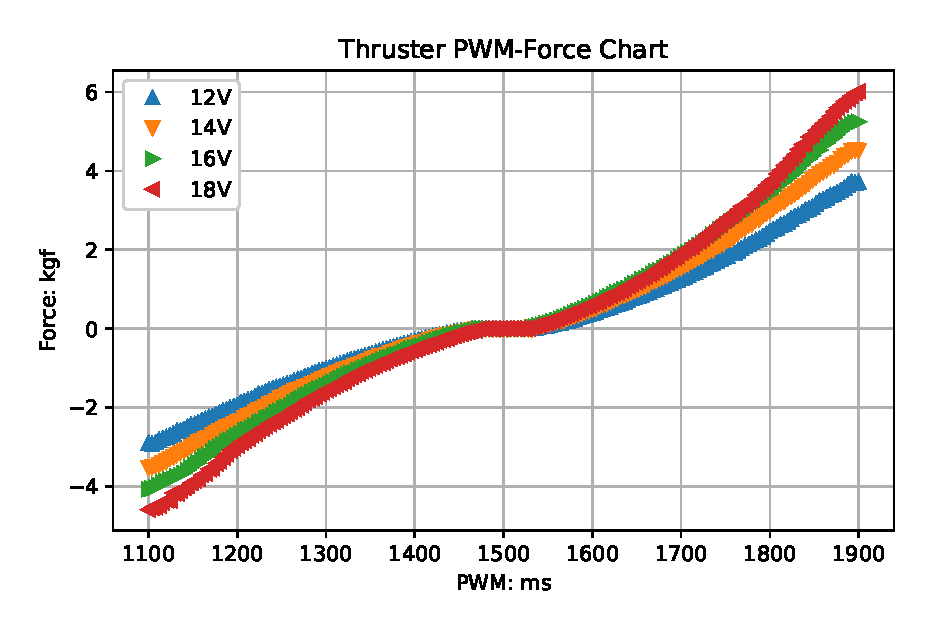
\includegraphics[width=\textwidth]{images/04thruster-curve.eps}
    \caption{BlueRobotics T200 Thruster input-output curve according to the lab test.}
    \label{fig:04thruster-curve}
\end{figure}

The input mapping part in the simulator transforms the input PWM values to the propulsion forces generated by the two thrusters. It works using the nearest point algorithm. At first, it determines which curve to look for the nearest point, then finds the dot with the closest PWM value.

\begin{equation}
    \boldsymbol{u}_{\rm f}=\boldsymbol{F}_{\Delta}(\boldsymbol{u}_{\rm PWM})
\end{equation}

The next step is to obtain the torque. According to the geometry definition of the thrusters, the torque can be calculated through the cross-product of the position vector and the propulsion force. 

\begin{equation}
    \boldsymbol{u}_{\rm q}=\boldsymbol{v_t}\times \boldsymbol{u}_{\rm f}
\end{equation}

And at last,

\begin{equation}
    \boldsymbol{\tau}=\left[\begin{array}{c}
        \boldsymbol{u}_{\rm f}  \\
        \boldsymbol{u}_{\rm q}
    \end{array}\right]
\end{equation}

Which is the right hand side of the EOM \cite{sonnenburg2013modeling}.

\section{Simulation Results}

After building the simulator, we tuned all parameters based on the position and speed data collected during the real-world tests to ensure the simulation was valid. Some parameters are fixed by the mechanical design, such as the gravity center and the mass matrix, so they are determined beforehand. 

Other parameters, including the water drag and skin friction coefficients and air drag coefficient (we set the simulator to have a zero skin coefficient for air skin friction), are changeable.

Readers can find three test results in the following few sections.

\subsection{Drop Test}

Drop test is the most straightforward test. In this test, we put Piranha at a certain height above the water at the beginning. When time starts, Piranha starts free-falling until it reaches a stable position where the buoyancy and weight are equal.

Because the input vector is zero all the time, this test can be used to verify the hydrostatic estimator and hydrodynamics estimator work properly. The results are shown in Figure \ref{fig:04drop-test-xyz}, \ref{fig:04drop-test-ptp}, \ref{fig:04drop-test-uvw}, \ref{fig:04drop-test-pqr}.

\begin{figure}[H]
    \centering
    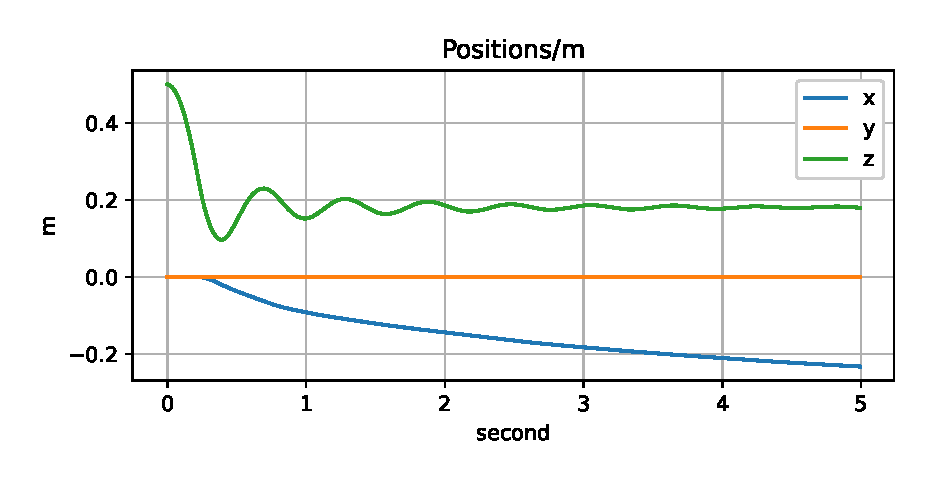
\includegraphics[width=.8\textwidth]{images/04drop-test-xyz.eps}
    \caption{Simulation: Drop test result - Positions $x, y,z$}
    \label{fig:04drop-test-xyz}
\end{figure}

\begin{figure}[H]
    \centering
    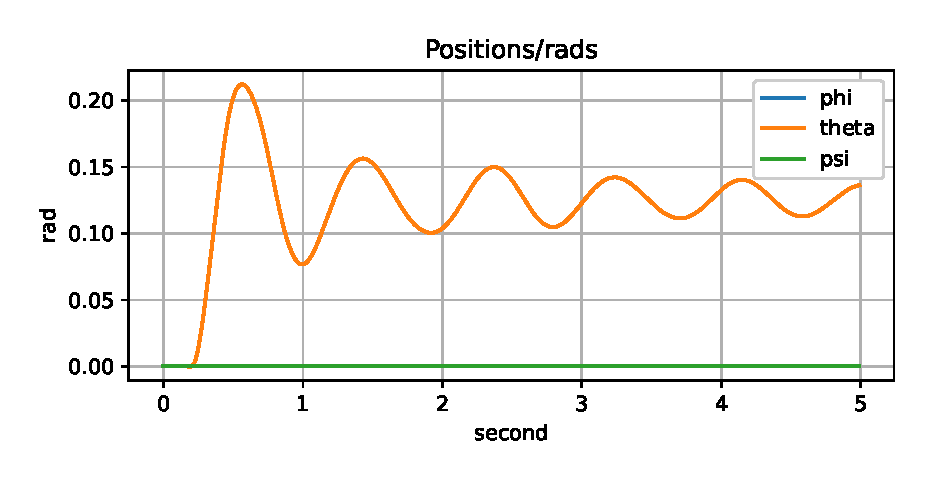
\includegraphics[width=.8\textwidth]{images/04drop-test-ptp.eps}
    \caption{Simulation: Drop test result - Attitude $\phi, \theta, \psi$}
    \label{fig:04drop-test-ptp}
\end{figure}

\begin{figure}[H]
    \centering
    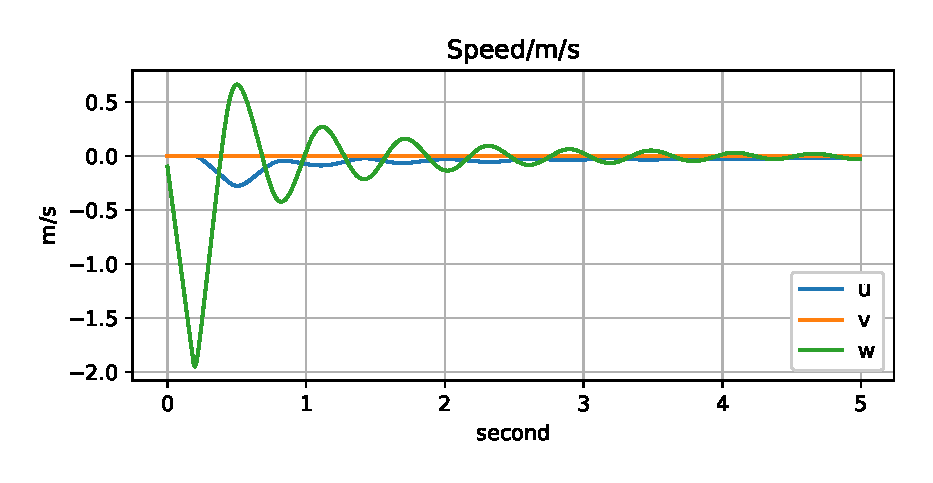
\includegraphics[width=.8\textwidth]{images/04drop-test-uvw.eps}
    \caption{Simulation: Drop test result - Linear Speed $u, v, w$}
    \label{fig:04drop-test-uvw}
\end{figure}

\begin{figure}[H]
    \centering
    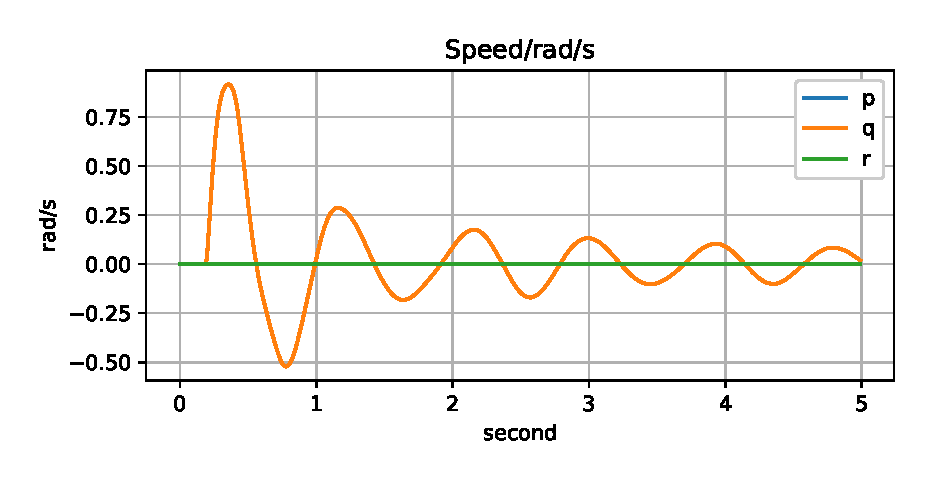
\includegraphics[width=.8\textwidth]{images/04drop-test-pqr.eps}
    \caption{Simulation: Drop test result - Angular Speed $p, q, r$}
    \label{fig:04drop-test-pqr}
\end{figure}

\subsection{Linear Driving Test}

In the Linear driving test, Piranha starts at a stable state, with a zero speed. When the test starts, the left and right thrusters move forward at maximum input values. The test results are shown in Figure \ref{fig:04linear-test-xyz}, \ref{fig:04linear-test-ptp}, \ref{fig:04linear-test-uvw}, \ref{fig:04linear-test-pqr}.

\begin{figure}[H]
    \centering
    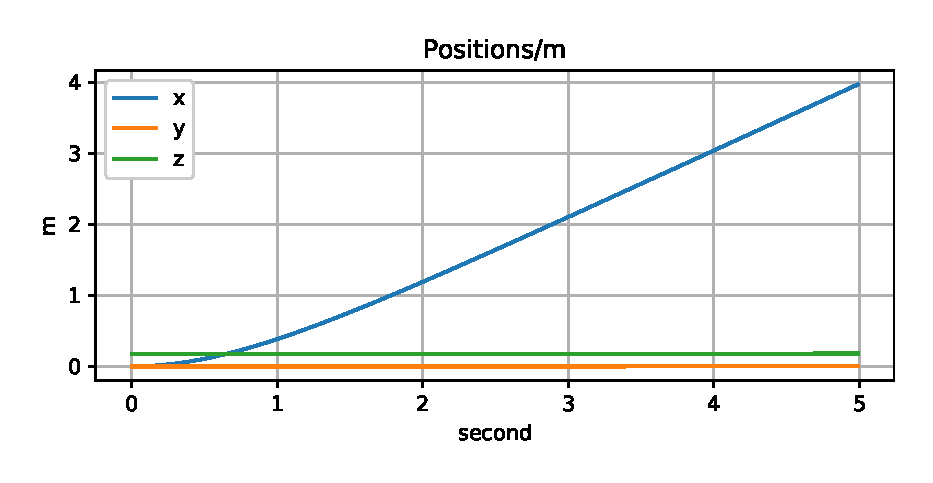
\includegraphics[width=.8\textwidth]{images/04linear-test-xyz.eps}
    \caption{Simulation: Linear driving test result - Positions $x, y,z$}
    \label{fig:04linear-test-xyz}
\end{figure}

\begin{figure}[H]
    \centering
    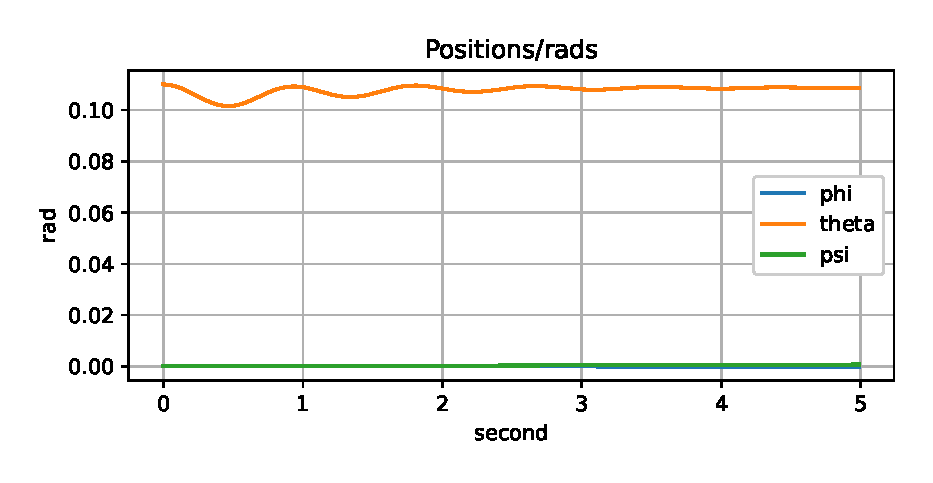
\includegraphics[width=.8\textwidth]{images/04linear-test-ptp.eps}
    \caption{Simulation: Linear driving test result - Attitude $\phi, \theta, \psi$}
    \label{fig:04linear-test-ptp}
\end{figure}

\begin{figure}[H]
    \centering
    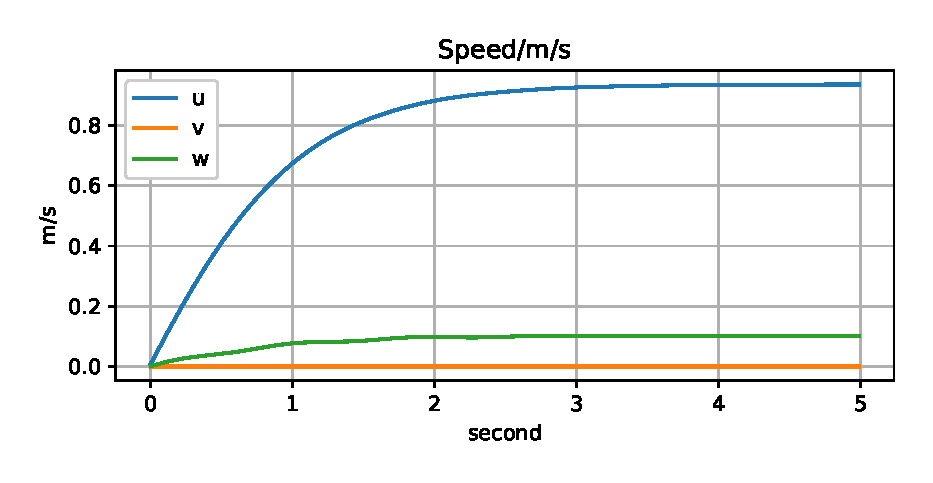
\includegraphics[width=.8\textwidth]{images/04linear-test-uvw.eps}
    \caption{Simulation: Linear driving test result - Linear Speed $u, v, w$}
    \label{fig:04linear-test-uvw}
\end{figure}

\begin{figure}[H]
    \centering
    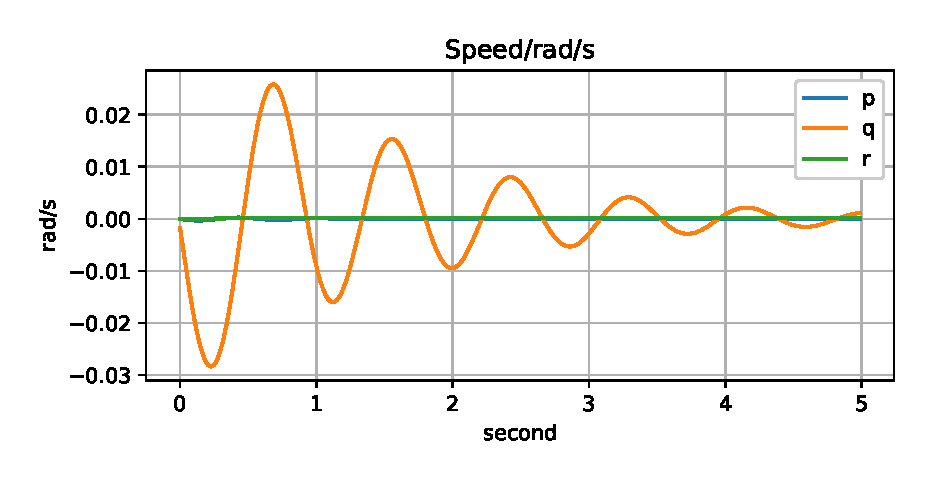
\includegraphics[width=.8\textwidth]{images/04linear-test-pqr.eps}
    \caption{Simulation: Linear driving test result - Angular Speed $p, q, r$}
    \label{fig:04linear-test-pqr}
\end{figure}

\subsection{Steering Test}

Steering test starts Piranha at the equilibrium point, then the left thruster is given a maximum forward input value, the right thruster is given a maximum backward input value. As a result, the Piranha starts turning. The simulation results can be found in Figure \ref{fig:04steer-test-xyz}, \ref{fig:04steer-test-ptp}, \ref{fig:04steer-test-uvw}, \ref{fig:04steer-test-pqr}.

\begin{figure}[H]
    \centering
    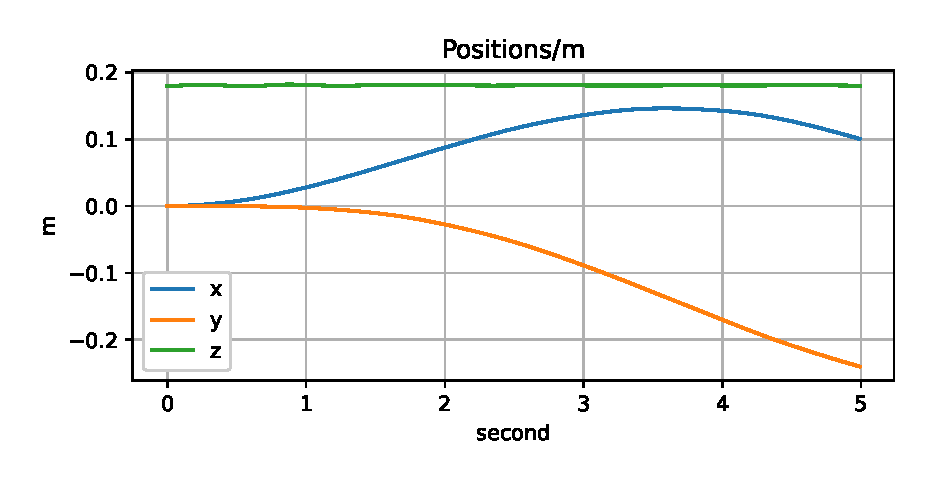
\includegraphics[width=.8\textwidth]{images/04steer-test-xyz.eps}
    \caption{Simulation: Steering test result - Positions $x, y,z$}
    \label{fig:04steer-test-xyz}
\end{figure}

\begin{figure}[H]
    \centering
    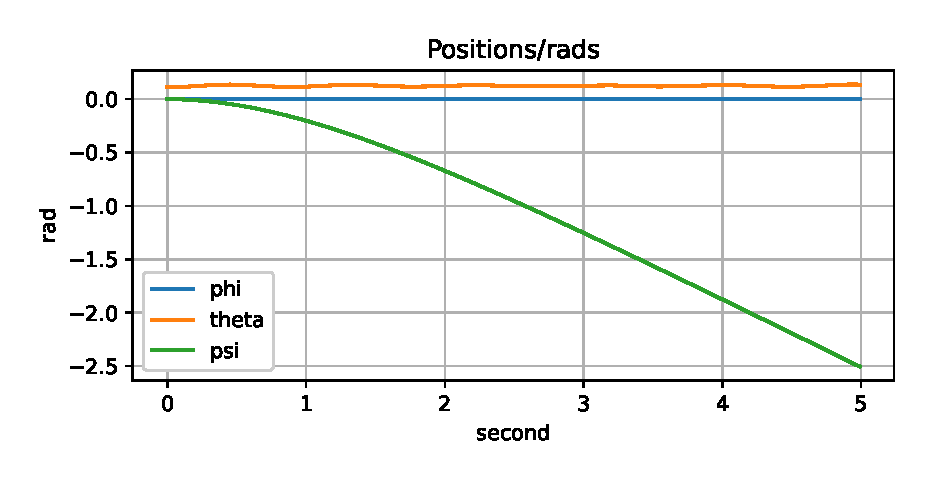
\includegraphics[width=.8\textwidth]{images/04steer-test-ptp.eps}
    \caption{Simulation: Steering test result - Attitude $\phi, \theta, \psi$}
    \label{fig:04steer-test-ptp}
\end{figure}

\begin{figure}[H]
    \centering
    \includegraphics[width=.8\textwidth]{images/04steer-test-uvw.eps}
    \caption{Simulation: Steering test result - Linear Speed $u, v, w$}
    \label{fig:04steer-test-uvw}
\end{figure}

\begin{figure}[H]
    \centering
    \includegraphics[width=.8\textwidth]{images/04steer-test-pqr.eps}
    \caption{Simulation: Steering test result - Angular Speed $p, q, r$}
    \label{fig:04steer-test-pqr}
\end{figure}

\chapter{Control System}

This chapter introduces Piranha's control system design. Unlike the simulation, where the model is 6-DoF and has a 3D environment, we based the control system design on a 3-DoF model representation, also called a navigation model. We did this because Piranha's vertical position is automatically controlled by the fluid physics. 

We also ignored the roll, pitch angles. During the field test, the collected data shows the pitch and roll angle of Piranha hardly changed. Readers can verify this fact in the simulation results.

\section{Navigation Model}

The navigation model is a 2D model rather than 3D. This is because the third position value, $z$, is not of the control system interested \cite{aastrom1976identification}. The model frame is shown in Figure \ref{fig:05nav-model}.

\begin{figure}[H]
    \centering
    \includegraphics[width=.6\textwidth]{images/05nav-model.pdf}
    \caption{Piranha navigation model and frame.}
    \label{fig:05nav-model}
\end{figure}

\subsection{Equation of Motion}

We can find the EOM of the navigation model:

\begin{equation}
    \boldsymbol{M}\dot{\boldsymbol{\nu}}+\boldsymbol{D}(\boldsymbol{\nu}, \boldsymbol{w})=\boldsymbol{\tau}
\end{equation}

Because $z,\ \phi,\ \theta$ are removed, only $p_n,\ p_e,\ \psi$ remains in the equation. The position state vector $\boldsymbol{x}_n$ and the velocity vector are defined as:

\begin{equation}
    \boldsymbol{x}_n=\left[\begin{array}{c}
        p_n  \\
        p_e  \\
        \psi
    \end{array}\right] \quad \boldsymbol{v}_n=\left[\begin{array}{c}
        u  \\
        v  \\
        r
    \end{array}\right]
\end{equation}

\subsection{Control Input}

The input vector is the same as the simulation EOM:

\begin{equation}
    \boldsymbol{\tau}=\left[\begin{array}{c}
        f_u  \\
        0 \\
        t_\tau
    \end{array}\right]=\boldsymbol{T}\left[\begin{array}{c}
        u_f  \\
        u_r 
    \end{array}\right]=\boldsymbol{T}\boldsymbol{F}_\Delta(\boldsymbol{u}_{\rm PWM})
\end{equation}

Here a new input pair $[f_f, t_r]$ is used to simplify the formulation, $f_f$ is the forward force, $t_r$ is the input torque, we can solve back from this new input vector to the original input vector simply. And with the new input representation, we have:

\begin{figure}
    \centering
    \includegraphics[width=.8\textwidth]{images/05input-loc.pdf}
    \caption{Thrusters' location with respect to the mass center.}
    \label{fig:05input-loc}
\end{figure}

\begin{equation}
    \boldsymbol{\tau}=\left[\begin{array}{cc}
        1 & 0 \\
        0 & 0\\
        0 & 1 
    \end{array}\right]\left[\begin{array}{c}
        f_f  \\
        t_r
    \end{array}\right]
\end{equation}

The reason why here a force-torque vector is the used, rather than the original PWM command vector, is that it does not break the linearity of the EOM, and on the other hand, we can search the PWM value the controller need back from the mapping function $\boldsymbol{F}_{\rm map}$. 

\begin{equation}
    \boldsymbol{u}_{\rm PWM}=\boldsymbol{F}_{\rm map}^{-1}\left(\left[\begin{array}{c}
        u_f  \\
        u_r
    \end{array}\right]\right)
\end{equation}

\subsection{Mass matrix}

The mass matrix can be written as:

\begin{equation}
    \boldsymbol{M}=\left[\begin{array}{ccc}
        m & 0 & 0 \\
        0 & m & 0 \\
        0 & 0 & I \\
    \end{array}\right]
\end{equation}

Where $m$ is the mass value of Piranha, and $I$ is the $z$ axis rotational inertia.

\subsection{Damping Matrix}

$\boldsymbol{D}(\boldsymbol{\nu})$ is the damping matrix and is much simpler than the one in simulation. We formulate it as:

\begin{equation}
    \boldsymbol{D}(\boldsymbol{\nu})=\left[\begin{aligned}
        -\frac{1}{2}A_f \rho_d u^2 & \\
        -\frac{1}{2}A_s \rho_d v^2 & \\
        -\frac{1}{2}A_I \rho_r r^2 &
    \end{aligned}\right]
\end{equation}

Where $A_f$, $A_s$, $A_I$ represent the Piranha's frontal area for $u$ $v$ and $r$ direction. $\rho_d$ is the second order drag coefficient and $\rho_r$ is the second order rotational drag coefficient.

In the end, the whole EOM can be found as:

\begin{align}
    \dot{\boldsymbol{x}} & =\left[\begin{array}{ccc}
        \cos{\psi} & -\sin{\psi} & 0  \\
        \sin{\psi} & \cos{\psi} & 0 \\
        0 & 0 & 1
    \end{array}\right]\boldsymbol{\nu} \\
    \dot{\boldsymbol{\nu}} & =\frac{1}{M}\left(\left[\begin{array}{cc}
        1 & 0 \\
        0 & 0\\
        0 & 1 
    \end{array}\right]\boldsymbol{F}_\Delta(\boldsymbol{u}_{\rm PWM})-\left[\begin{aligned}
        -\frac{1}{2}A_f \rho_d u^2 & \\
        -\frac{1}{2}A_s \rho_d v^2 & \\
        -\frac{1}{2}A_I \rho_r r^2 &
    \end{aligned}\right]\right)
\end{align}

We can see that only the $u$ and $\psi$ are controllable. The side-way speed, $v$, is constantly deteriorating because of the resistance.

\section{Extended Kalman Filter}

Piranha is equipped with multiple sensors, including two accelerometers, two gyroscopes, three magnetometers, one GPS. In such a situation, we developed an Extended Kalman Filter (EKF) for Piranha to use all the measurements to estimate the boat's position, velocity, and orientation. The full python script is attached to the Appendix \ref{app:ekf-sympy} for a better understanding of the structure of the EKF on Piranha. The mathematical formulation follows the latest EKF paper \cite{bortz1971new}, and I followed the software design criteria written on the engineering practice \cite{savage1998strapdown1, savage1998strapdown2}.

Two EKF instances run parallel on the two IMUs and output two results for the estimated states. The final result of the estimator depends on the ICM20948 EKF instance. However, another value called result credibility is calculated based on the difference between the two EKF outputs, and it decides if the EKF result is valid in the run time.

\subsection{States and Observations}

The EKF used on Piranha has 13 state variables in the state vector. These variables include:

\begin{itemize}
    \item $[q_0,q_1,q_2,q_3]$ 4 quaternions which define the orientation.
    \item $[v_n,v_e,v_d]$ NED velocity vector.
    \item $[p_n,p_e,p_d]$ NED position vector.
    \item $[{\rm mag}_N, {\rm mag}_E, {\rm mag}_D]$ NED earth fixed magnetic field components.
\end{itemize}

\begin{figure}[ht]
    \centering
    \includegraphics[width=.8\textwidth]{images/05ekf-flowchart.pdf}
    \caption{The overall EKF flowchart on Piranha.}
    \label{fig:05ekf-flowchart}
\end{figure}

\subsection{State Predict}

After getting a new set of raw data from the IMUs, the algorithm first predicts the update on the quaternions $q_0,q_1,q_2,q_3$, and the position $p_n,p_e,p_d$ in the NED frame. First the program does the following steps:

\begin{enumerate}
    \item Get raw readings from each IMU. These raw readings include the acceleration values $\Delta v_x, \Delta v_y, \Delta v_z$ from each accelerometer, and the angular speed values $\Delta a_x, \Delta a_y, \Delta a_z$ from each gyroscope.
    \item Feed the raw readings to the running integrators, save the previously estimated state vector, and check the predicted state vector's output. During this time, the values in the error matrix (sometimes called state covariance matrix $P[t+1]$) also grow.
\end{enumerate}

\subsubsection{IMU Prediction Equation}

The observation variables of the IMU includes:

\begin{itemize}
    \item $[\Delta a_x, \Delta a_y, \Delta a_z]$ Delta angular positions in the $XYZ$ frame ($xyz$ accelerations).
    \item $[\Delta v_x, \Delta v_y, \Delta v_z]$ Delta velocity in the $XYZ$ frame ($xyz$ angular velocities).
\end{itemize}

We can write the prediction equations or the discretized EOM as:

\begin{equation}
        \left[\begin{array}{c}
            v_n  \\
            v_e  \\
            v_d
        \end{array}\right]_{[t+1]}=\left[\begin{array}{c}
            v_n  \\
            v_e  \\
            v_d
        \end{array}\right]_{[t]}+\quad\left[\begin{array}{c}
            g_n  \\
            g_e  \\
            g_d
        \end{array}\right]_{[t]}{\Delta t}+Q(q_0,q_1,q_2,q_3)*\left[\begin{array}{c}
            \Delta v_x  \\
            \Delta v_y  \\
            \Delta v_z
        \end{array}\right]\Delta t_{[t]}
\end{equation}

\begin{equation}
        \left[\begin{array}{c}
            p_n  \\
            p_e  \\
            p_d
        \end{array}\right]_{[t+1]}=\left[\begin{array}{c}
            p_n  \\
            p_e  \\
            p_d
        \end{array}\right]_{[t]}+\quad\left[\begin{array}{c}
            v_n  \\
            v_e  \\
            v_d
        \end{array}\right]_{[t]}{\Delta t}
\end{equation}

\begin{equation}
        \left[\begin{array}{c}
            q_0  \\
            q_1  \\
            q_2  \\
            q_3
        \end{array}\right]_{[t+1]}=\left[\begin{array}{c}
            q_0  \\
            q_1  \\
            q_2  \\
            q_3
        \end{array}\right]_{[t]} \bigotimes\quad \left[\begin{array}{c}
            \cos{\frac{\theta}{2}}  \\
            \frac{\boldsymbol{\omega}_x}{\left\lVert\boldsymbol{\omega}\right\rVert} \sin \frac{\theta}{2}  \\
            \frac{\boldsymbol{\omega}_y}{\left\lVert\boldsymbol{\omega}\right\rVert} \sin \frac{\theta}{2}  \\
            \frac{\boldsymbol{\omega}_z}{\left\lVert\boldsymbol{\omega}\right\rVert} \sin \frac{\theta}{2}  \\
        \end{array}\right]_{[t]}\approx\quad \left[\begin{array}{c}
            q_0  \\
            q_1  \\
            q_2  \\
            q_3
        \end{array}\right]_{[t]}\bigotimes\quad \left[\begin{array}{c}
            1  \\
            0.5\Delta a_x\Delta t  \\
            0.5\Delta a_y\Delta t  \\
            0.5\Delta a_z\Delta t  \\
        \end{array}\right]_{[t]}
\end{equation}

The $[{\rm mag}_N, {\rm mag}_E, {\rm mag}_D]$ prediction equation is very simple. As we know, the earth's magnetic field barely changes locally, so the EKF predicts that these three values keep constant:

\begin{equation}
    \left[\begin{array}{c}
            \Tilde{\rm mag}_N  \\
            \Tilde{\rm mag}_E  \\
            \Tilde{\rm mag}_D
        \end{array}\right]_{[t+1]}=\left[\begin{array}{c}
            {\rm mag}_N  \\
            {\rm mag}_E  \\
            {\rm mag}_D
        \end{array}\right]_{[t]}
\end{equation}


Where $g_n,g_e,g_d$ are the gravity components in NED frame, $\mathcal{F}$ is the quaternion multiplication function.


After getting the discretized EOM, EKF calculates the Jacobian of the EOM $\boldsymbol{F}_j$ using the built-in python function \mintinline{python}{jacobian()}. Then it is used to update the covariance matrix:

\begin{equation}
    \boldsymbol{P}[t+1]=\boldsymbol{F}_j \boldsymbol{P}[t+1] {\boldsymbol{F}^\top}_j+\boldsymbol{Q}_k
\end{equation}

\subsection{Attitude Update}

Although the gyroscope provides information about the rotation angles, we need an extra step to align the starting position with the earth-fixed NED system to have the correct yaw angle. In other words, to make the North axis point to the geographical north pole. This alignment is essential for marine navigation. To do so, EKF needs a compass or magnetometer.

An extra highly sensitive magnetometer RM3100 is installed at the boat's head to generate precise yaw angle measurement.  

When EKF sees a new magnetometer measurement, the measurement is  in the body frame, so the observation function is:

\begin{equation}
    \textbf{mag}_{ob}=h(\boldsymbol{x}_{\rm EKF})=R_{\rm quat}(q_0,q_1,q_2,q_3)^\top \left[\begin{array}{c}
            \rm mag_N  \\
            \rm mag_E  \\
            \rm mag_D
        \end{array}\right]_{[t+1]}
\end{equation}

The predicted observation:

\begin{equation}
    \Tilde{\textbf{mag}}_{ob}=h(\boldsymbol{x}_{\rm EKF})=R_{\rm quat}(\Tilde{q_0},\Tilde{q_1},\Tilde{q_2},\Tilde{q_3})^\top \left[\begin{array}{c}
            \Tilde{\rm mag}_N  \\
            \Tilde{\rm mag}_E  \\
            \Tilde{\rm mag}_D
        \end{array}\right]_{[t+1]}
\end{equation}

EKF updates the attitude through:

\begin{align}
    \Delta \textbf{mag}_{ob} & =\textbf{mag}_{ob}-\Tilde{\textbf{mag}}_{ob} \\
    \textbf{H}_k &=\left.\frac{\partial h}{\partial \boldsymbol{x}}\right|_{\Tilde{x}_k} \\
    \textbf{S}_k &=\textbf{H}_k\textbf{P}_k\textbf{H}_k^\top+\textbf{R}_k \\
    \textbf{K}_k &=\textbf{P}_k\textbf{H}_k^\top\textbf{S}^{-1} \\
    \Tilde{\boldsymbol{x}}_k &=\Tilde{\boldsymbol{x}}_k+\textbf{K}_k\Delta\Tilde{\textbf{mag}}_{ob} \\
    \textbf{P}_k &=(\textbf{I}-\textbf{K}_k\textbf{H}_k)\textbf{P}_k
\end{align}

It will update both the stored magnetic field vector ${\rm mag}_N, {\rm mag}_E, {\rm mag}_D$ and the quaternions $[q0, q1, q2, q3]$.

\subsubsection{Body Magnetic Field}

In the discussion above, the calculation only considers the earth's magnetic field. However, in reality, the circuit on Piranha will inevitably create a magnetic field in the body frame. Adding the body's magnetic vector to the state vector list reduces the noise of the attitude update. However, because we installed the magnetometer on Piranha far from the electrical parts, we ignored the effect of the body's magnetic field. 


\subsection{Position Update}

EKF enters this step when there is a new position reading on the GPS sensor, a standard GPS message \textbf{\$GPSGGA} of the NMEA format contains the following information:

\begin{itemize}
    \item UTC Time.
    \item Latitude.
    \item North/South Indicator.
    \item Longitude.
    \item West/East Indicator.
\end{itemize}

The NED position measurement $p_{n{\rm GPS}},\ p_{e{\rm GPS}},\ p_{d{\rm GPS}}$ is calculated based on the latitude and longitude values first. Then it will be the observation state:

\begin{equation}
    \boldsymbol{y}_{ob}=\left[\begin{array}{c}
        p_n  \\
        p_e  \\
        p_d  \\
    \end{array}\right]
\end{equation}

So the innovation step is:

\begin{align}
    \Delta \boldsymbol{y}_{ob} & =\boldsymbol{y}_{ob}-\Tilde{\boldsymbol{y}}_{ob} \\
    \textbf{H}_k &=\left.\frac{\partial h}{\partial \boldsymbol{x}}\right|_{\Tilde{x}_k} \\
    \textbf{S}_k &=\textbf{H}_k\textbf{P}_k\textbf{H}_k^\top+\textbf{R}_k \\
    \textbf{K}_k &=\textbf{P}_k\textbf{H}_k^\top\textbf{S}^{-1} \\
    \Tilde{\boldsymbol{x}}_k &=\Tilde{\boldsymbol{x}}_k+\textbf{K}_k\Delta \boldsymbol{y}_{ob} \\
    \textbf{P}_k &=(\textbf{I}-\textbf{K}_k\textbf{H}_k)\textbf{P}_k
\end{align}

Because GPS measurements are not always available, this step will be skipped if the GPS module loses fix on the satellite and fails to obtain a new measure. In such a situation, the error matrix $P_k$ starts growing in the repeated predict steps, meaning the error accumulates in the estimated states.

\subsection{EKF Results}

Figure \ref{fig:05ekf-result-linear} and \ref{fig:05ekf-result-turn} show two EKF estimated trajectories and the raw GPS test data. We did these tests using the simulation program discussed in the previous section. We can see that, in the simulation, the EKF on Piranha can estimate the trajectory correctly even with huge GPS noise.

\begin{figure}[H]
    \centering
    \includegraphics[width=.8\textwidth]{images/05ekf-result-linear.eps}
    \caption{EKF estimated trajectory versus raw GPS data in the linear driving simulation.}
    \label{fig:05ekf-result-linear}
\end{figure}

\begin{figure}[H]
    \centering
    \includegraphics[width=.8\textwidth]{images/05ekf-result-turn.eps}
    \caption{EKF estimated trajectory versus raw GPS data in the steering simulation.}
    \label{fig:05ekf-result-turn}
\end{figure}

\section{PD Controller for Yaw Control}

Because there are errors in many ways, like we did not properly align the thrusters during the assembly, or one thruster is weaker than the other, the boat cannot drive in a straight line without a closed-loop controller. So a controller for yaw control driving is needed. On Piranha, A simple PD controller is implemented for this purpose. 

The key to linear driving is to keep the headings stable. We can see the structure of the PD controller in Figure \ref{fig:05pid-flowchart}.

\begin{figure}[H]
    \centering
    \includegraphics[width=.8\textwidth]{images/05pid-flowchart.pdf}
    \caption{Piranha PD heading controller flowchart.}
    \label{fig:05pid-flowchart}
\end{figure}

The PD equation is:

\begin{align}
    f_f &= k_{p1}(u-\Tilde{u}) \\
    t_r &= k_{p2}(0-\Tilde{\psi})+k_{p3}(0-\Tilde{r})+k_{d}(0- \frac{{\rm d}\Tilde{r}}{{\rm d}t})
\end{align}

After getting the $f_f$ and $t_r$, the controller solves the raw input using the reversed input mapping function:

\subsection{Test Results}

A simple test can show how the PD controller works. In the test, we reduced the left thruster's maximum power output to 80\%. Meanwhile, the right thruster is still at 100\% of the original. In real life, it is common that some ropes or plastic wastes get caught on the thruster protector and drag the left thruster down, or it is simply because the output power is different between the two thrusters due to design defections. However, we can see in Figure \ref{fig:05nopid-xyz}, \ref{fig:05nopid-ptp}, \ref{fig:05nopid-uvw}, \ref{fig:05nopid-pqr}, \ref{fig:05nopid-input} that without a PD controller, the heading $\psi$ keeps increasing, making the boat drive to the left.

\begin{figure}[ht]
    \centering
    \includegraphics[width=.8\textwidth]{images/05nopid-test-xyz.eps}
    \caption{Simulation: Without the PD controller - Positions $x, y, z$.}
    \label{fig:05nopid-xyz}
\end{figure}

\begin{figure}[ht]
    \centering
    \includegraphics[width=.8\textwidth]{images/05nopid-test-ptp.eps}
    \caption{Simulation: Without the PD controller - Positions $\phi, \theta, \psi$.}
    \label{fig:05nopid-ptp}
\end{figure}

\begin{figure}[ht]
    \centering
    \includegraphics[width=.8\textwidth]{images/05nopid-test-uvw.eps}
    \caption{Simulation: Without the PD controller - Linear Speed $u, v, w$.}
    \label{fig:05nopid-uvw}
\end{figure}

\begin{figure}[ht]
    \centering
    \includegraphics[width=.8\textwidth]{images/05nopid-test-pqr.eps}
    \caption{Simulation: Without the PD controller - Angular Speed $p, q, r$.}
    \label{fig:05nopid-pqr}
\end{figure}

\begin{figure}[ht]
    \centering
    \includegraphics[width=.8\textwidth]{images/05nopid-test-input.eps}
    \caption{Simulation: Without the PD controller - Inputs $u_l, u_r$.}
    \label{fig:05nopid-input}
\end{figure}

With the PD controller, the input of the two thrusters are automatically calculated based on the observation to decrease the error in the heading $\psi$. The results improved by a lot, the $\psi$ stays within a small deviation range, and the drift on the $y$ direction is eliminated. The test results can be seen in Figure \ref{fig:05pid-xyz}, \ref{fig:05pid-ptp}, \ref{fig:05pid-uvw}, \ref{fig:05pid-pqr}, \ref{fig:05pid-input}.

\begin{figure}[H]
    \centering
    \includegraphics[width=.8\textwidth]{images/05pid-test-xyz.eps}
    \caption{Simulation: With the PD controller - Positions $x, y, z$.}
    \label{fig:05pid-xyz}
\end{figure}

\begin{figure}[H]
    \centering
    \includegraphics[width=.8\textwidth]{images/05pid-test-ptp.eps}
    \caption{Simulation: With the PD controller - Positions $\phi, \theta, \psi$.}
    \label{fig:05pid-ptp}
\end{figure}

\begin{figure}[H]
    \centering
    \includegraphics[width=.8\textwidth]{images/05pid-test-uvw.eps}
    \caption{Simulation: With the PD controller - Linear Speed $u, v, w$.}
    \label{fig:05pid-uvw}
\end{figure}

\begin{figure}[H]
    \centering
    \includegraphics[width=.8\textwidth]{images/05pid-test-pqr.eps}
    \caption{Simulation: With the PD controller - Angular Speed $p, q, r$.}
    \label{fig:05pid-pqr}
\end{figure}

\begin{figure}[H]
    \centering
    \includegraphics[width=.8\textwidth]{images/05pid-test-input.eps}
    \caption{Simulation: With the PD controller - Inputs $u_l, u_r$.}
    \label{fig:05pid-input}
\end{figure}

\section{Trajectory Tracking}

In the previous section, the PD controller can control the forward speed $u$ and the heading position $\psi$. However, the PD controller itself is not enough for Piranha to track a trajectory. This section explains the experimental trajectory tracking controller on Piranha. It was designed based on the feedback linearization theory. However, it did have the ability to correct the error one a specific direction.

In the future, I am going to test reinforcement learning and model predictive control. Previous research showed good results by using these two methods\cite{woo2018dynamic}, \cite{cuiarticle}, \cite{naeemarticle}.


\subsection{Feedback Linearization Controller}

\begin{figure}[H]
    \centering
    \includegraphics[width=.8\textwidth]{images/05fl-flowchart.pdf}
    \caption{Piranha's trajectory tracking feedback linearization controller flowchart.}
    \label{fig:05fl-flowchart}
\end{figure}

Readers can check the feedback linearization algorithm workflow in Figure \ref{fig:05fl-flowchart}. The previous section brought the EOM of the navigation model, which can be simplified as:

\begin{align}
    \dot{\boldsymbol{x}} & =\left[\begin{array}{ccc}
        \cos{\psi} & -\sin{\psi} & 0  \\
        \sin{\psi} & \cos{\psi} & 0 \\
        0 & 0 & 1
    \end{array}\right]\boldsymbol{\nu} \\
    \dot{\boldsymbol{\nu}} & =\frac{1}{M}\left(\left[\begin{array}{cc}
        1 & 0 \\
        0 & 0\\
        0 & 1 
    \end{array}\right]\boldsymbol{u}_f-\left[\begin{aligned}
        -\frac{1}{2}A_f \rho_d u^2 & \\
        -\frac{1}{2}A_s \rho_d v^2 & \\
        -\frac{1}{2}A_I \rho_d r^2 &
    \end{aligned}\right]\right)
\end{align}

To construct the feedback linearization vector, we can construct the state vector as:

\begin{equation}
    \boldsymbol{x}_l=\left[\begin{array}{c}
        p_n  \\
        p_e  \\
        \psi \\
    \end{array}\right]
\end{equation}

The observation vector is the same as the state vector with the EKF estimator brought in in the previous section.

\begin{equation}
    \boldsymbol{y}_l=\boldsymbol{x}_l
\end{equation}

Since it is a second-order system, construct a feedback vector $\boldsymbol{z}$, so that:



\begin{equation}
    \boldsymbol{z}=T(\boldsymbol{x}_l)=\left[\begin{array}{c}
        \boldsymbol{x}_l  \\
        \dot{\boldsymbol{x}}_l
    \end{array}\right]
\end{equation}

We can find the $\dot{\boldsymbol{x}}_l$ from the early EOM. Because we can directly observe the velocity vector $\boldsymbol{\nu}$ in the body frame, so its vector form is reserved. The $\ddot{\boldsymbol{x}}_l$ can be found as:

\begin{equation}
    \ddot{\boldsymbol{x}}_l=\left[\begin{array}{ccc}
        -\sin{\dot{\psi}} & -\cos{\dot{\psi}} & 0  \\
        \cos{\dot{\psi}} & -\sin{\dot{\psi}} & 0 \\
        0 & 0 & 0
    \end{array}\right]\boldsymbol{\nu}+\left[\begin{array}{ccc}
        \cos{\psi} & -\sin{\psi} & 0  \\
        \sin{\psi} & \cos{\psi} & 0 \\
        0 & 0 & 1
    \end{array}\right]\dot{\boldsymbol{\nu}}
\end{equation}

In the $\dot{\boldsymbol{\nu}}$ the input vector can be found. Define the new input of the system to be $\boldsymbol{v}$, So that the $\boldsymbol{v}$ is a linear function of $\boldsymbol{u}_f$:

\begin{equation}
    \ddot{\boldsymbol{x}}_l=f_l(\boldsymbol{u}_f)=\boldsymbol{A}_l\cdot\boldsymbol{u}_f+\boldsymbol{b}_l
\end{equation}

Which turns the given system into a linearized system with a cascade of integrators:

\begin{equation}
    \begin{split}
        \dot{\boldsymbol{z}}_1 &= z_2 \\
        \dot{\boldsymbol{z}}_2 &= \ddot{\boldsymbol{x}}_l
    \end{split}
\end{equation}

By the control law, in such a linearized system, the control vector $v$ can be found as:

\begin{equation}
    \boldsymbol{v}=-K\boldsymbol{z}
\end{equation}

After finding the control vector $\boldsymbol{v}$, the original control vector $\boldsymbol{u}_f$ can be found using the reverse mapping from $u_f\rightarrow v$.

\begin{equation}
    \boldsymbol{u}_f=A^+(\boldsymbol{v}-\boldsymbol{b})
\end{equation}

Because the matrix $A$ is not invertible, $A^+$ denotes the pseudo-inverse of the $A$ matrix. However, the primary error of the feedback linearization controller arises in this step. To explain it, we first find that:

\begin{equation}
    \left[\begin{array}{cc}
        1 & 0 \\
        0 & 0 \\
        0 & 1
    \end{array}\right]^+=\left[\begin{array}{ccc}
        1 & 0 & 0\\
        0 & 0 & 1\\
    \end{array}\right]
\end{equation}

The equation means the error in the second variable of the state $[u,\ v,\ w]$, i.e., the velocity at the $v$ direction is ignored while multiplying this matrix. We can explain this error by the fact that the system cannot control the $v$ variable. As a result, the error in the side-way direction accumulated during the trajectory, which can be seen in the next section.

\subsubsection{Circle Trajectory Result}

The first test is the circle trajectory test, the results are showed in the following Figures \ref{fig:05fl-result-circle}, \ref{fig:05fl-result-circle-xyz}, \ref{fig:05fl-result-circle-ptp},\ref{fig:05fl-result-circle-uvw},\ref{fig:05fl-result-circle-pqr}, \ref{fig:05fl-result-circle-u}. 

\begin{figure}[H]
    \centering
    \includegraphics[width=.5\textwidth]{images/05fl-result-circle.eps}
    \caption{Feedback linearization trajectory tracking controller test result, the reference is a circle trajectory.}
    \label{fig:05fl-result-circle}
\end{figure}

\begin{figure}[H]
    \centering
    \includegraphics[width=.8\textwidth]{images/05fl-result-circle-xyz.eps}
    \caption{Feedback linearization trajectory tracking controller test result - Position $x,\ y,\ z$.}
    \label{fig:05fl-result-circle-xyz}
\end{figure}

\begin{figure}[H]
    \centering
    \includegraphics[width=.8\textwidth]{images/05fl-result-circle-ptp.eps}
    \caption{Feedback linearization trajectory tracking controller test result - Attitude $\phi,\ \theta,\ \psi$.}
    \label{fig:05fl-result-circle-ptp}
\end{figure}

\begin{figure}[H]
    \centering
    \includegraphics[width=.8\textwidth]{images/05fl-result-circle-uvw.eps}
    \caption{Feedback linearization trajectory tracking controller test result - Linear Speed $u,\ v,\ w$.}
    \label{fig:05fl-result-circle-uvw}
\end{figure}

\begin{figure}[H]
    \centering
    \includegraphics[width=.8\textwidth]{images/05fl-result-circle-pqr.eps}
    \caption{Feedback linearization trajectory tracking controller test result - Angular Speed $p,\ q,\ r$.}
    \label{fig:05fl-result-circle-pqr}
\end{figure}

\begin{figure}[H]
    \centering
    \includegraphics[width=.8\textwidth]{images/05fl-result-circle-u.eps}
    \caption{Feedback linearization trajectory tracking controller test result - Input $u_l,\ u_r$.}
    \label{fig:05fl-result-circle-u}
\end{figure}

\subsubsection{Square Trajectory Result}

The second test has a square-shaped trajectory. Compared with the circle trajectory, there are discontinuities at each vertex of the square at the reference velocity and heading. In this test, we can see that the feedback linearization controller can correct the yaw angle. However, it cannot reduce the error in the $v$ direction since the input $u_l,\ u_r$ does not control $v$ directly.

\begin{figure}[H]
    \centering
    \includegraphics[width=.5\textwidth]{images/05fl-result-square.eps}
    \caption{Feedback linearization trajectory tracking controller test result, the reference is a square trajectory.}
    \label{fig:05fl-result-square}
\end{figure}

\begin{figure}[H]
    \centering
    \includegraphics[width=.8\textwidth]{images/05fl-result-square-xyz.eps}
    \caption{Feedback linearization trajectory tracking controller test result - Position $x,\ y,\ z$.}
    \label{fig:05fl-result-square-xyz}
\end{figure}

\begin{figure}[H]
    \centering
    \includegraphics[width=.8\textwidth]{images/05fl-result-square-ptp.eps}
    \caption{Feedback linearization trajectory tracking controller test result - Attitude $\phi,\ \theta,\ \psi$.}
    \label{fig:05fl-result-square-ptp}
\end{figure}

\begin{figure}[H]
    \centering
    \includegraphics[width=.8\textwidth]{images/05fl-result-square-uvw.eps}
    \caption{Feedback linearization trajectory tracking controller test result - Linear Speed $u,\ v,\ w$.}
    \label{fig:05fl-result-square-uvw}
\end{figure}

\begin{figure}[H]
    \centering
    \includegraphics[width=.8\textwidth]{images/05fl-result-square-pqr.eps}
    \caption{Feedback linearization trajectory tracking controller test result - Angular Speed $p,\ q,\ r$.}
    \label{fig:05fl-result-square-pqr}
\end{figure}

\begin{figure}[H]
    \centering
    \includegraphics[width=.8\textwidth]{images/05fl-result-square-u.eps}
    \caption{Feedback linearization trajectory tracking controller test result - Input $u_l,\ u_r$.}
    \label{fig:05fl-result-square-u}
\end{figure}

We can see that the feedback linearization controller can navigate Piranha to drive towards the expected trajectory. However, because it only considers the error at present, it cannot eliminate the error at the $v$ direction, which requires the controller to have the ability to plan. 

\chapter{Conclusion}

This report describes the water surface robot, Piranha. The first chapter covers the initial concept of Piranha and compares multiple available trash collection options before Piranha's configuration is finally determined. The second chapter tells the reader how we built the Piranha from simple mechanical parts. The third chapter illustrates the electrical system that powers the Piranha and the specifications of all components and their verification. The fourth chapter proposes a new way to formulate a dynamic model for a water surface vehicle and provides the numerical methods needed on the computer.  The fifth chapter first introduces a 13-state EKF based on the modern control theory and then a PD controller for heading and speed control. At the end of the fifth chapter, this report describes a feedback linearization controller to achieve the trajectory tracking function on Piranha.

The simulation brought in chapter four is based on several existing designs. Because it reads the model as a triangle mesh, it does not care about the configurations of the watercraft. Additionally, the simulation results have a very high precision because it uses a more precise frontal area estimate algorithm based on the sliced triangle faces. 

We keep a balance between complexity and speed for the EKF discussed in chapter five. It shows good stability even under considerable GPS noise. There is a possibility of increasing the state vector length and acquiring better precision. However, the EKF will also lose its speed simultaneously.

This report also serves as an entry-level engineering practice guidance for anyone who wants to build an RC vehicle, either a car, drone, or boat, in the real world. It includes concept development, mechanical design, electrical design, simulation, and the control system design, all essential sections for a successful robot design.

\section{Future work}

Although it is still at prototyping stage, Piranha will be a commercial product and eventually be on the market. So the most critical work for the mechanical and electrical design in the next step is to simplify the manufacturing process and speed up the production meanwhile reducing the fabrication cost for each unit. This work includes customizing plastic molds and drawing PCBs.

On the safety aspect, electromagnetic interference (EMI) and several fail-safe routines need to be designed in the next step to ensure the electrical system's stability and the operators' safety. Also, as a marine robot, it needs to meet the same industry standards for a common watercraft, such as the signal lights and other proper indicators.

There is still a lot of space for improvement in the control section, like using reinforcement learning and model predictive controllers for better tracking results. They are not discussed in this report because they are still under development at this moment. In the next step, more control approaches will be developed, and their performance will be investigated.

%%%%%%%%%%%%%%%%%%%%%%%%%%%%%%%%%%%%%%%%%%%
% Appendices
%%%%%%%%%%%%%%%%%%%%%%%%%%%%%%%%%%%%%%%%%%%

\appendix

\label{app:t200}

\chapter{BlueRobotics Thruster T200 Data}
%% This shows appendix shows how to attach a file to the appendix.

\begin{figure}[H]
    \centering
    \includegraphics[width=.85\textwidth]{images/app-t200-12v.pdf}
    \caption{T200 Public Performance Data 10-20V, 12 V}
\end{figure}

\begin{figure}[H]
    \centering
    \includegraphics[width=.85\textwidth]{images/app-t200-14v.pdf}
    \caption{T200 Public Performance Data 10-20V, 14 V}
\end{figure}

\begin{figure}[H]
    \centering
    \includegraphics[width=.85\textwidth]{images/app-t200-16v.pdf}
    \caption{T200 Public Performance Data 10-20V, 16 V}
\end{figure}

\begin{figure}[H]
    \centering
    \includegraphics[width=.85\textwidth]{images/app-t200-18v.pdf}
    \caption{T200 Public Performance Data 10-20V, 18 V}
\end{figure}

\label{app:ekf-sympy}
\chapter{Piranha EKF SymPy Script}

In the application, the essential EKF functions such as the Kalman gain functions, are generated first using a computer algebra system (CAS) called \mintinline{python}{SymPy} and the results are saved. This \mintinline{python}{SymPy} script will take about 5~10 minutes on a modern PC to finish. EKF function blocks are saved into separated binary files using the Python \mintinline{python}{dill} tool.

\renewcommand{\baselinestretch}{1}\selectfont
\begin{minted}{python}
## Piranha EKF Symbolic Computation Script
# Author: Xiahua Liu
# Last Modified Date: 10/13/2021
# Description: This script generates the EKF functions in numpy
# format and saves them in binary files with the dill library
# The EKF invented in this script has 13 states.
# This script takes around 5~10 minutes on a modern computer.

from sympy import *
from sympy.algebras.quaternion import Quaternion

# Dill the result functions to disks
import dill
dill.settings['recurse'] = True

## Define state variables
# IMU delta angle measurements in body axes - rad
dax, day, daz = symbols("da_x, da_y, da_z", real=True)
# IMU delta velocity measurements in body axes - m/sec
dvx, dvy, dvz = symbols("dv_x, dv_y, dv_z", real=True)
# Quaternions
q0, q1, q2, q3 = symbols("q_0, q_1, q_2, q_3", real=True)
# NED velocity - m/sec
vn, ve, vd = symbols("v_n, v_e, v_d", real=True)   
# NED position - m
pn, pe, pd = symbols("p_n, p_e, p_d", real=True)  
# IMU time step 
dt = symbols("dt", real=True)    
# NED gravity vector - m/sec^2
g = symbols("g", real=True)    
# NED earth fixed magnetic field components - milligauss
magN, magE, magD = symbols("mag_N, mag_E, mag_D", real=True)    

P = MatrixSymbol('P', 13, 13) # P matrix
Q = MatrixSymbol('Q', 13, 13) # Q matrix
R_mag = MatrixSymbol('R_mag', 1,1) # R mag 
R_gps = MatrixSymbol('R_gps', 1,1) # R gps postion 

# Define the state vector
stateVector = Matrix([q0, q1, q2, q3, vn, ve, vd, pn, pe, pd, magN, magE, magD])

# Meaured angle speed and acceleration
da = Matrix([dax, day, daz])
dv = Matrix([dvx, dvy, dvz])

# Quaternion vector & rotation matrix
quat = Quaternion(q0, q1, q2, q3)
Tbn = quat.to_rotation_matrix()

# NED Gravity calculation
gvec=Matrix([0,0,g], real=True)


## Predict Step
# Quaternion update equation
delQuat = Quaternion(1, 0.5*dax*dt, 0.5*day*dt, 0.5*daz*dt)
quatNew = quat.mul(delQuat)

# Velocity update equation
vNew = Matrix([vn, ve, vd])+gvec*dt+Tbn*dv*dt

# Position update equation
pNew = Matrix([pn, pe, pd])+Matrix([vn, ve, vd])*dt

# Earth magnetic field update equation
magNew = Matrix([magN, magE, magD])

# Process equation
processEqn = Matrix([quatNew.a, quatNew.b, quatNew.c, quatNew.d, vNew, pNew, magNew])


## Innovation Step
# Linearized state transition matrix
F=simplify(processEqn.jacobian(stateVector))

# Pack into lambda objects
F_lambda=lambdify((q0,q1,q2,q3,dvx,dvy,dvz,dax,day,daz,dt), F, 'numpy')
# Dill the lambda functions
dill.dump(F_lambda, open("F_lambda.npf", "wb"))

# New covariance matrix
PP=simplify(F*P*F.T+Q)

# Pack into lambda objects
PP_lambda=lambdify((q0,q1,q2,q3,dvx,dvy,dvz,dax,day,daz,dt, P, Q, g), PP, 'numpy')
# Dill the lambda functions
dill.dump(PP_lambda, open("PP_lambda.npf", "wb"))


## Mag measurement fusion
magMeas=Tbn.T*Matrix([magN, magE, magD])

# Mag measurement jacobian
H_mag=simplify(magMeas.jacobian(stateVector))

# Mag observation funciton
H_magx=H_mag[0,:]
H_magy=H_mag[1,:]
H_magz=H_mag[2,:]

# Kalman gains for mag fustion
K_mx=simplify((P*H_magx.T)/(H_magx*P*H_magx.T+R_mag))
K_my=simplify((P*H_magy.T)/(H_magy*P*H_magy.T+R_mag))
K_mz=simplify((P*H_magz.T)/(H_magz*P*H_magz.T+R_mag))

# GPS measurement jacobian
H_gps=simplify(Matrix([pn, pe, pd]).jacobian(stateVector))

# GPS observation function
H_gpsn=H_gps[0,:]
H_gpse=H_gps[1,:]
H_gpsd=H_gps[2,:]

# Kalman gains for GPS fustion
K_pn=simplify((P*H_gpsn.T)/(H_gpsn*P*H_gpsn.T+R_gps))
K_pe=simplify((P*H_gpse.T)/(H_gpse*P*H_gpse.T+R_gps))
K_pd=simplify((P*H_gpsd.T)/(H_gpsd*P*H_gpsd.T+R_gps))


## Pack result function into lambda objects
# Pack into lambda objects
H_magx_lambda=lambdify((q0,q1,q2,q3, magN, magE, magD), H_magx, 'numpy')
H_magy_lambda=lambdify((q0,q1,q2,q3, magN, magE, magD), H_magy, 'numpy')
H_magz_lambda=lambdify((q0,q1,q2,q3, magN, magE, magD), H_magz, 'numpy')

# Dill the lambda functions
dill.dump(H_magx_lambda, open("H_magx_lambda.npf", "wb"))
dill.dump(H_magy_lambda, open("H_magy_lambda.npf", "wb"))
dill.dump(H_magz_lambda, open("H_magz_lambda.npf", "wb"))

# Pack into lambda objects
H_gpsn_lambda=lambdify((), H_gpsn, 'numpy')
H_gpse_lambda=lambdify((), H_gpse, 'numpy')
H_gpsd_lambda=lambdify((), H_gpsd, 'numpy')

# Dill the lambda functions
dill.dump(H_gpsn_lambda, open("H_gpsn_lambda.npf", "wb"))
dill.dump(H_gpse_lambda, open("H_gpse_lambda.npf", "wb"))
dill.dump(H_gpsd_lambda, open("H_gpsd_lambda.npf", "wb"))

# Pack into lambda objects
K_mx_lambda=lambdify((q0,q1,q2,q3,magN,magE,magD, P, R_mag), K_mx, 'numpy')
K_my_lambda=lambdify((q0,q1,q2,q3,magN,magE,magD, P, R_mag), K_my, 'numpy')
K_mz_lambda=lambdify((q0,q1,q2,q3,magN,magE,magD, P, R_mag), K_mz, 'numpy')

# Dill the lambda functions
dill.dump(K_mx_lambda, open("K_mx_lambda.npf", "wb"))
dill.dump(K_my_lambda, open("K_my_lambda.npf", "wb"))
dill.dump(K_mz_lambda, open("K_mz_lambda.npf", "wb"))

# Pack into lambda objects
K_pn_lambda=lambdify((P,R_gps), K_pn, 'numpy')
K_pe_lambda=lambdify((P,R_gps), K_pe, 'numpy')
K_pd_lambda=lambdify((P,R_gps), K_pd, 'numpy')

# Dill the lambda functions
dill.dump(K_pn_lambda, open("K_pn_lambda.npf", "wb"))
dill.dump(K_pe_lambda, open("K_pe_lambda.npf", "wb"))
dill.dump(K_pd_lambda, open("K_pd_lambda.npf", "wb"))
\end{minted}


%%%%%%%%%%%%%%%%%%%%%%%%%%%%%%%%%%%%%%%%%%%
% Bibliography
%%%%%%%%%%%%%%%%%%%%%%%%%%%%%%%%%%%%%%%%%%%

\bibliographystyle{plain}
\bibliography{references}

\end{document}
